\documentclass[11pt,twoside]{report}

% some definitions for the title page
\newcommand{\reporttitle}{Transfer Learning in Computer-Assisted Contouring for Radiotherapy Planning} % Transfer Learning in Computer-Assisted Contouring for Radiotherapy Planning

\newcommand{\reportauthor}{Anton Zhitomirsky}
\newcommand{\supervisor}{Prof Ben Glocker}
\newcommand{\secondMarker}{Dr Thomas Heinis}
\newcommand{\reporttype}{MEng Individual Project}

% load some definitions and default packages
%%%%%%%%%%%%%%%%%%%%%%%%%%%%%%%%%%%%%%%%%
% University Assignment Title Page 
% LaTeX Template
% Version 1.0 (27/12/12)
%
% This template has been downloaded from:
% http://www.LaTeXTemplates.com
%
% Original author:
% WikiBooks (http://en.wikibooks.org/wiki/LaTeX/Title_Creation)
%
% License:
% CC BY-NC-SA 3.0 (http://creativecommons.org/licenses/by-nc-sa/3.0/)
% 
%
%%%%%%%%%%%%%%%%%%%%%%%%%%%%%%%%%%%%%%%%%
%----------------------------------------------------------------------------------------
%	PACKAGES AND OTHER DOCUMENT CONFIGURATIONS
%----------------------------------------------------------------------------------------
\usepackage[a4paper,hmargin=2.0cm,vmargin=1.0cm,includeheadfoot]{geometry}
\usepackage{textpos}

\usepackage[square,numbers]{natbib} % for bibliography
\usepackage[nottoc]{tocbibind} % Includes "References" in the table of contents
\bibliographystyle{unsrtnat}

\usepackage{tabularx,longtable,multirow,subfigure,caption}%hangcaption
\usepackage{fancyhdr} % page layout
\usepackage{url} % URLs
\usepackage[english]{babel}
\usepackage{amsmath}
\usepackage{graphicx}
\usepackage{scalerel}
\usepackage{dsfont}
\usepackage{epstopdf} % automatically replace .eps with .pdf in graphics
\usepackage{backref} % needed for citations
\usepackage{array}
\usepackage{latexsym}

\usepackage[pdftex,pagebackref,hypertexnames=false,colorlinks]{hyperref} % provide links in pdf
\usepackage{booktabs}
\usepackage{wrapfig}
\usepackage{caption}  % Required for \captionof
\usepackage{float} % for H option in figures
\usepackage{amssymb}
\usepackage{amsmath}
\usepackage{csquotes}
% \usepackage{subcaption} % causes a compilation error after changing back to natbib referencing... 

\hypersetup{pdftitle={},
  pdfsubject={}, 
  pdfauthor={},
  pdfkeywords={}, 
  pdfstartview=FitH,
  pdfpagemode={UseOutlines},% None, FullScreen, UseOutlines
  bookmarksnumbered=true, bookmarksopen=true, colorlinks,
    citecolor=black,%
    filecolor=black,%
    linkcolor=black,%
    urlcolor=black}

\usepackage[all]{hypcap}

%%%%%%%%%%%%%%%%%%%%%%%%%%%%%%%%%%%%%%%%%%%%%%%%%%%%%%%%%%%%%%%%%%%%%%%%%%%%%%%%
% LISTINGS ammendments
%%%%%%%%%%%%%%%%%%%%%%%%%%%%%%%%%%%%%%%%%%%%%%%%%%%%%%%%%%%%%%%%%%%%%%%%%%%%%%%%
\usepackage{listings}

\lstset
{ %Formatting for code in appendix
    language=Matlab,
    basicstyle=\footnotesize,
    % numbers=left,
    stepnumber=1,
    showstringspaces=false,
    tabsize=1,
    breaklines=true,
    breakatwhitespace=false,
    frame=single,
    columns=fullflexible,
    postbreak=\mbox{\textcolor{red}{$\hookrightarrow$}\space},
}

%\usepackage{color}
%\usepackage[tight,ugly]{units}
%\usepackage{float}
%\usepackage{tcolorbox}
%\usepackage[colorinlistoftodos]{todonotes}
% \usepackage{ntheorem}
% \theoremstyle{break}
% \newtheorem{lemma}{Lemma}
% \newtheorem{theorem}{Theorem}
% \newtheorem{remark}{Remark}
% \newtheorem{definition}{Definition}
% \newtheorem{proof}{Proof}


%%% Default fonts
\renewcommand*{\rmdefault}{bch}
\renewcommand*{\ttdefault}{cmtt}


%%% Default settings (page layout)
\setlength{\parindent}{0em}  % indentation of paragraph
\setlength{\parskip}{.3em}

% \setlength{\parindent}{0em}  % indentation of paragraph

\setlength{\headheight}{14.5pt}
\pagestyle{fancy}
\renewcommand{\chaptermark}[1]{\markboth{\chaptername\ \thechapter.\ #1}{}}
%\fancyhead[RO]{\sffamily \textbf{\thepage}} %Page no.in the right on even pages
%\fancyhead[LE]{\sffamily \textbf{\thepage}} %Page no. in the left on odd pages

\fancyfoot[ER,OL]{\thepage}%Page no. in the left on
%odd pages and on right on even pages
\fancyfoot[OC,EC]{\sffamily }
\renewcommand{\headrulewidth}{0.1pt}
\renewcommand{\footrulewidth}{0.1pt}
\captionsetup{margin=10pt,font=small,labelfont=bf}


%--- chapter heading

\def\@makechapterhead#1{%
  \vspace*{10\p@}%
  {\parindent \z@ \raggedright \sffamily
    \interlinepenalty\@M
    \Huge\bfseries \thechapter \space\space #1\par\nobreak
    \vskip 30\p@
  }}

%--- chapter heading

\def\@makechapterhead#1{%
  \vspace*{10\p@}%
  {\parindent \z@ \raggedright \sffamily
    %{\Large \MakeUppercase{\@chapapp} \space \thechapter}
    %\\
    %\hrulefill
    %\par\nobreak
    %\vskip 10\p@
    \interlinepenalty\@M
    \Huge\bfseries \thechapter \space\space #1\par\nobreak
    \vskip 30\p@
  }}

%---chapter heading for \chapter*  
\def\@makeschapterhead#1{%
  \vspace*{10\p@}%
  {\parindent \z@ \raggedright
    \sffamily
    \interlinepenalty\@M
    \Huge \bfseries  #1\par\nobreak
    \vskip 30\p@
  }}
\allowdisplaybreaks

% load some macros
% Here, you can define your own macros. Some examples are given below.

\newcommand{\R}[0]{\mathds{R}} % real numbers
\newcommand{\Z}[0]{\mathds{Z}} % integers
\newcommand{\N}[0]{\mathds{N}} % natural numbers
\newcommand{\C}[0]{\mathds{C}} % complex numbers
% \renewcommand{\vec}[1]{{\boldsymbol{{#1}}}} % vector
\newcommand{\mat}[1]{{\boldsymbol{{#1}}}} % matrix

\usepackage{pifont,mdframed}
\newenvironment{warning}
  {\par\begin{mdframed}[linewidth=1pt,linecolor=black]%
    \begin{list}{}{\leftmargin=1cm
                  \labelwidth=\leftmargin}\item[\Large\ding{43}]}
  {\end{list}\end{mdframed}\par}

\definecolor{lightgray}{gray}{0.9}
\usepackage[T1]{fontenc}

% load title page
\begin{document}
% Last modification: 2015-08-17 (Marc Deisenroth)
\begin{titlepage}

    \newcommand{\HRule}{\rule{\linewidth}{0.5mm}} % Defines a new command for the horizontal lines, change thickness here
    
    %----------------------------------------------------------------------------------------
    %	LOGO SECTION
    %----------------------------------------------------------------------------------------
    
    
\includegraphics[width = 4cm]{../figures/imperial.pdf}\\[0.5cm] 
    
    \center % Center everything on the page
     
    %----------------------------------------------------------------------------------------
    %	HEADING SECTIONS
    %----------------------------------------------------------------------------------------
    
    \textsc{\LARGE \reporttype}\\[1.5cm] 
    \textsc{\Large Department of Computing}\\[0.5cm] 
    \textsc{\large Imperial College of Science, Technology and Medicine}\\[0.5cm] 
    
    %----------------------------------------------------------------------------------------
    %	TITLE SECTION
    %----------------------------------------------------------------------------------------
    
    \HRule \\[0.4cm]
    { \huge \bfseries \reporttitle}\\ % Title of your document
    \HRule \\[1.5cm]
     
    %----------------------------------------------------------------------------------------
    %	AUTHOR SECTION
    %----------------------------------------------------------------------------------------
    
    \begin{minipage}{0.4\textwidth}
    \begin{flushleft} \large
    \emph{Author:}\\
    \reportauthor % Your name
    \end{flushleft}
    \end{minipage}
    ~
    \begin{minipage}{0.4\textwidth}
    \begin{flushright} \large
    \emph{Supervisor:} \\
    \supervisor % Supervisor's Name
    \end{flushright}
    \end{minipage}\\[4cm]
    
    
    
    
    %----------------------------------------------------------------------------------------
    
    
    %----------------------------------------------------------------------------------------
    %	DATE SECTION
    %----------------------------------------------------------------------------------------
    
    {\large \today} % Date, change the \today to a set date if you want to be precise
    
    
    \vfill % Fill the rest of the page with whitespace
    Submitted in partial fulfillment of the requirements for the \degreetype~of Imperial College London
    
    \end{titlepage}
    

% page numbering etc.
\pagenumbering{roman}
\clearpage{\pagestyle{empty}\cleardoublepage}
\setcounter{page}{1}
\pagestyle{fancy}


% \cleardoublepage
%%%%%%%%%%%%%%%%%%%%%%%%%%%%%%%%%%%%
% \section*{Acknowledgments}
% Comment this out if not needed.

% \clearpage{\pagestyle{empty}\cleardoublepage}

%%%%%%%%%%%%%%%%%%%%%%%%%%%%%%%%%%%%

\begin{abstract}\label{sect:abstract}
  Radiotherapy planning involves outlining the macro and microscopic spreads of a cancer. Previously, bespoke models were trained on sufficient sample sizes of architectures that vary significantly in design to address distinct segmentation objectives. However, this makes models inaccessible to departments with limited datasets, increasing the barrier to experiencing the promised superiority beyond a model's specific use case.

  We, therefore, analyse the effectiveness of transfer learning techniques in leveraging knowledge learned from one domain into another. Variants of transfer include zero-shot, few-shot and many-shot transfer learning. The evaluation of n-shot approaches of transfer learning onto the radiotherapy planning objective will clarify whether the transfer is a valid strategy for increasing performance over models learnt from scratch.
  % TODO: Add more about the results
  We represent three distinct model architectures for each type of transfer. We conclude that a many-shot transfer using TotalSegmentator remains a robust method for transfering knowledge. We find that few-shot transfer using UinverSeg does not apply to the complexity of 3-D volume delineations for cervical cancer. Finally, the finetuning of zero-shot models, represented by MedSAM, offers local bounded improvements on volume delineation independently of tumour localisation when compared to the baseline.

  % The repo is available at \url{https://github.com/AntonZhitomirsky/radiotherapy}.
\end{abstract}
  
%%%%%%%%%%%%%%%%%%%%%%%%%%%%%%%%%%%%
%--- table of contents
\fancyhead[RE,LO]{\sffamily {Table of Contents}}
\tableofcontents
  
% \clearpage{\pagestyle{empty}\cleardoublepage}

%%%%%%%%%%%%%%%%%%%%%%%%%%%%%%%%%%%%

\pagenumbering{arabic}
\setcounter{page}{1}
\fancyhead[LE,RO]{\slshape \rightmark}
\fancyhead[LO,RE]{\slshape \leftmark}

%%%%%%%%%%%%%%%%%%%%%%%%%%%%%%%%%%%%
\chapter{Introduction}

\section{Technical Context}

% Transfer Learning is a technique in which a model trained on one task is repurposed and fine-tuned on a second task. Thus, the model can leverage the knowledge gained from the first task to improve performance on the second task. 


Currently, the most common network architecture backbone for radiotherapy planning is the U-Net architecture~\cite{Samarasinghe2021-ps, Lin2021-oz, Sartor2020-et, LIU2020184, Rhee2020-ms, LIU2020172}. However, each network requires specialized architectures or bespoke training schemes to achieve competitive performance. These tailored modifications contribute little to the overall development in medical segmentation~\cite{isensee2024nnunet}, as it becomes increasingly challenging for researchers to identify methods that live up to their promised superiority beyond the limited scenarios they are demonstrated on~\cite{nnunet}.

Furthermore, the bespoke architectures assume a sufficient sample size representing a sound representation of the population of all individuals under the same circumstances. However, the underrepresented users of these models cannot apply this assumption; most hospital teams work in a specialized medical field with only in-house patients who follow specific hospital guidelines. A simple plug-and-play approach is unsuitable because segmentation guidelines often differ between facilities. Therefore, specific recalibration is necessary to effectively use these models because incorrect or inaccurate contours are the primary factors contributing to treatment failures in radiotherapy~\cite{Rhee2020-ms}.

\section{Objective and Methodology}

We therefore analyse the effectiveness of Transfer Learning in radiotherapy planning. The Transfer Learning approach aims to leverage other trained models with great performance and lift low-level features for the target domain. A PubMed accrual for deep learning solutions in radiotherapy planning found a gap in technical research surrounding Transfer Learning in the radiotherapy planning field\footnote{Search string used in the PubMed accrual in 2023-2024 is available at Figure~\ref{fig:pubmed-search-string}}. Therefore, research on transfer in the medical domain will also fill the literature gap, which has yet to consider transfer learning as a solution for radiotherapy planning volumes. 

Firstly, we select a dataset from The Royal Marsden Hospital, which will act as the pillar for advocating the success and use of transfer learning in radiotherapy planning. The real-world clinical dataset provides segmentations for key anatomies and tumours that aid in radiotherapy planning for females with cervical cancer. It has yet to gain exposure to the public segmentation community and has uncommon and limited segmentation patterns specified by internal team-wide guidelines.

Secondly, we analyse the effectiveness of transfer learning in radiotherapy planning. To research the application of this technique in the medical context, we utilize three popular architectures and their applications in transfer learning. These models are nnUNet~\cite{nnunet}, UniverSeg~\cite{universeg}, and MedSAM~\cite{Ma2024}. In tandem with the effectiveness of transferring knowledge from these models, we comment on the type of transfer, be it zero-shot, few-shot, or many-shot learning.

\section{Results}

% TODO

\section{Outline of Report}

The report will commence by delving into the essential background knowledge needed for this project in Chapter~\ref{sect:motivation}. This chapter provides a high-level overview of anatomies and the clinical context (Section~\ref{sect:clinical-context}), as well as the fundamental existing academic knowledge in the field of Computer-assisted vision in Medical Imaging (Section~\ref{sect:machine-learning-for-image-segmentation}).

Following this, Chapter~\ref{sect:methodology} will detail the experiments utilized to assess the effectiveness of different architectures in transferring knowledge into the target domain. Chapter~\ref{sect:results} presents and dissects the results of the experiment as well as their implications onto the medical community. Finally, Chapter~\ref{sect:conclusion} will cover the conclusion and future work Chapter~\ref{sect:conclusion}.

%%%%%%%%%%%%%%%%%%%%%%%%%%%%%%%%%%%%
\chapter{Motivation}\label{sect:motivation}

\section{Clinical Context}\label{sect:clinical-context}

This project will have its foundation for experimentation in a dataset provided by the Royal Marsden Hospital~\cite{AMLART-data}. The real-world clinical dataset segments key anatomies and tumours that aid in radiotherapy planning for females with cervical cancer. It has yet to gain exposure to the public eye and has uncommon and limited segmentation patterns. This dataset will act as the pillar for justifying the success of the transferability of knowledge between medical domains.

In this section, we discuss the clinical context behind cervical cancer in the population, the Hospital's pipeline for segmenting patients in preparation for radiotherapy treatment, and the Hospital's motivation for recruiting an AI tool to assist in its treatment pipeline. 

\subsection{Cervical Cancer}\label{sect:cervical-cancer}

Cancer is a burden around the globe that has been a driver for almost one-sixth of the world's mortality in 2022~\cite{Global-cancer-2022}. In females, cervical cancer makes up 25 countries' leading causes of cancer death, following breast cancer for 157 countries in 2022~\cite{Global-cancer-2022}. Furthermore, an estimated 1 million maternal orphans who lose their mothers to cancer suffer long-term disadvantages in health and education~\cite{Guida2022}. Thankfully, cancer screening services provided by hospitals around Europe have been shown to decrease incidence and mortality rates of cervical cancer in women over the recent years~\cite{Global-cancer-2022}. Paired with quality improvements offered by medical imaging models, this forms the motivation for total control over cervical cancer.

\subsection{Radiotherapy Treatment}

Radiation therapy is an option for cancer treatment where high beams of radiation energy are tuned to hone in to target cancerous cells in a clinically defined `target area'. The cells killed by the energy experience interphase or proliferative death depending on the cell cycle stage. Death occurs when the damage to genetic material within the cell prevents it from dividing, or the cell's accumulation of genetic aberrations leads to a ``mitotic catastrophe''~\cite{cell-death}. In Europe, such radiotherapy treatment was used on average for 70\% of cases, with a curative rate of 40\%~\cite{radiotherapy-advances, Thompson2018}.

All cells subjected to high-energy beams experience death. This places much responsibility on the oncologist to deliver an accurate treatment area so that healthy cells are unaffected, as the compromise of healthy cells' function may cause adverse alterations to an organ's standard functionality.

% This death is characteristic of any cell subjected to high energy beams, placing much responsibility on the oncologist to deliver an accurate treatment area so that healthy cells are unaffected; any adverse alteration of an organ's standard functionality may cause grave implications for the already compromised patient. 

Therefore, the care required causes oncologists to spend 90--120 mins to delineate target areas for radiotherapy~\cite{LIU2020184}. This time-consuming endeavour is never favourable for a patient already in a dangerous situation. For mid-low-income countries, where this may not be an available resource, this leaves them with a death rate 18 times that of a higher-income country~\cite{cervical-cancer-epidemic}. 

\subsection{CT modality and Hounsfield Units}\label{sect:ct-modality}

High-resolution and high-contrast computed tomography (CT) machines have further benefited cancer treatment due to their noninvasive nature and ability to view patients' internal organs. X-ray devices rotate around a specified body part, and computer-generated cross-sectional images are produced~\cite{file-formats}. Whilst the scanner rotates, the patient's table slowly moves up and down inside the tube to produce different cross-section images. The images show damaged and surrounding soft tissue, allowing physicians to propose clinical target volumes more accurately.

\begin{figure}[H]
    \centering
    \subfigure[Muscle Window $(35,55)$~\cite{other-HD-units}]{{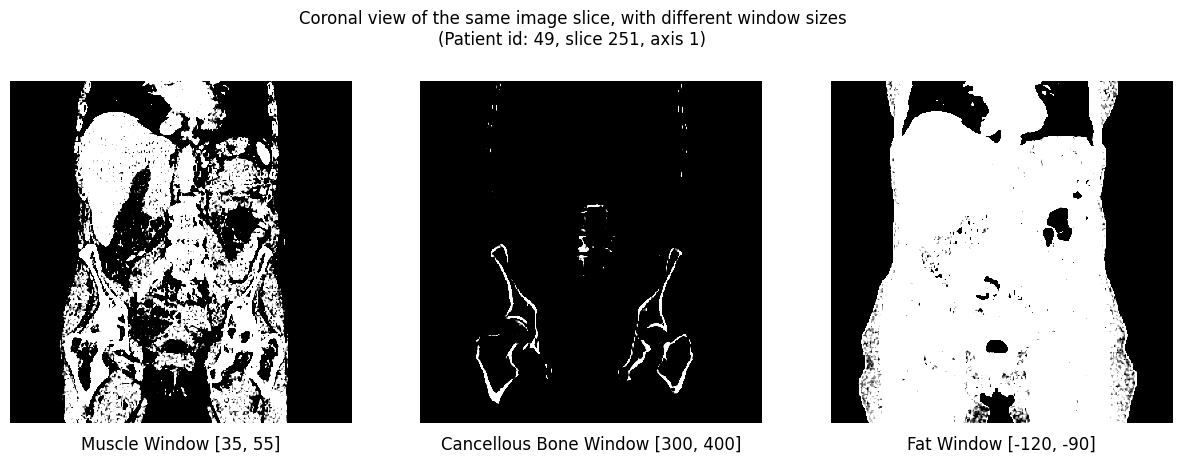
\includegraphics[width=0.3\textwidth, trim=0.2cm 1cm 21cm 2cm, clip]{../figures/HU-window.png}}}
    \subfigure[Bone Window  $(300,400)$~\cite{cancellous-bone}]{{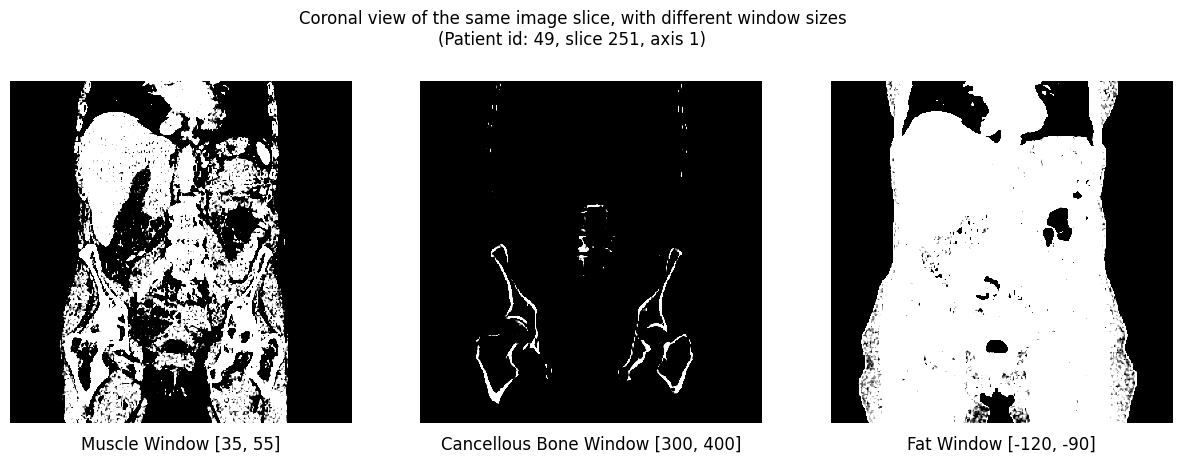
\includegraphics[width=0.3\textwidth, trim=10.6cm 1cm 10.6cm 2cm, clip]{../figures/HU-window.png}}}
    \subfigure[Fat Window $(-120, -90)$~\cite{other-HD-units}]{{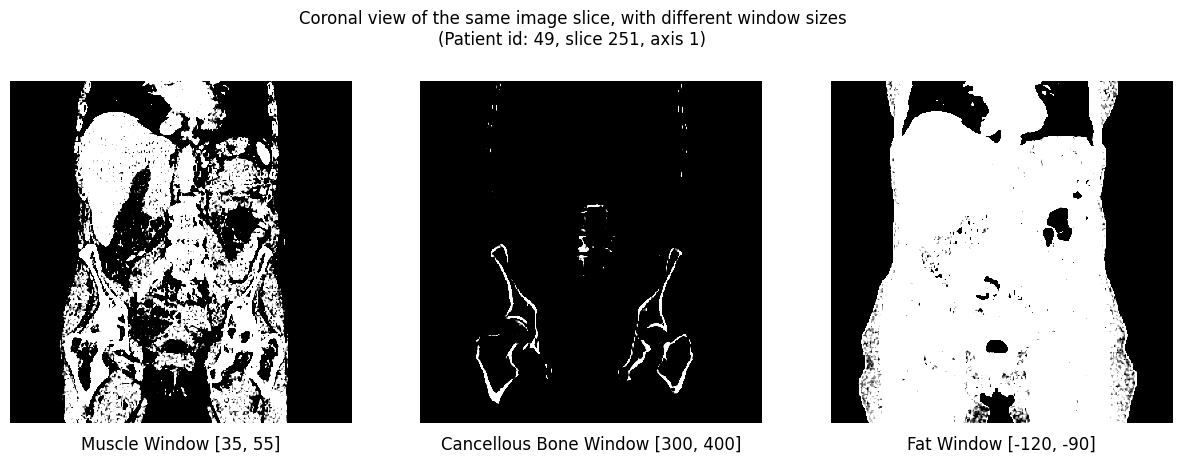
\includegraphics[width=0.3\textwidth, trim=21cm 1cm 0.2cm 2cm, clip]{../figures/HU-window.png}}}
    \caption{Coronal view the same image slice of a CT image, with different window cropping (Patient id: 49, slice 251). White (radiopaque) areas represent high-density tissues, and black (radiolucent) areas represent low-density tissues within the window range.}\label{fig:ct-windows}
\end{figure}

The operator or physician selects the image slice thickness from 1mm to 10mm. This choice determines the resolution of the image, with the cubes (voxels) measuring Hounsfield Units (HU)~\cite{diagnostic-radiology-physics}. The Hounsfield scale is a quantitative scale used in medical imaging to describe radiodensity. Unlike natural images, where the pixel's intensity determines a colour's intensity between 0 and 255, the voxel's intensity reflects the average tissue type for the cube and ranges between -1000 and 3000. Positive values (white) indicate denser tissue with greater X-ray beam absorption, while negative values (black) represent less dense tissue with less X-ray beam absorption~\cite{Statpearls}.

Therefore, because the HU scale is relative; different windows may be taken for a CT scan to highlight different tissues. Those voxels within the window will likely be tissues of a specific classification. An example is illustrated in Figure~\ref{fig:ct-windows}.

\subsection{Radiotherapy Planning}\label{sect:radiotherapy-planning}

\begin{figure}[H]
  \subfigure[GTV]{
    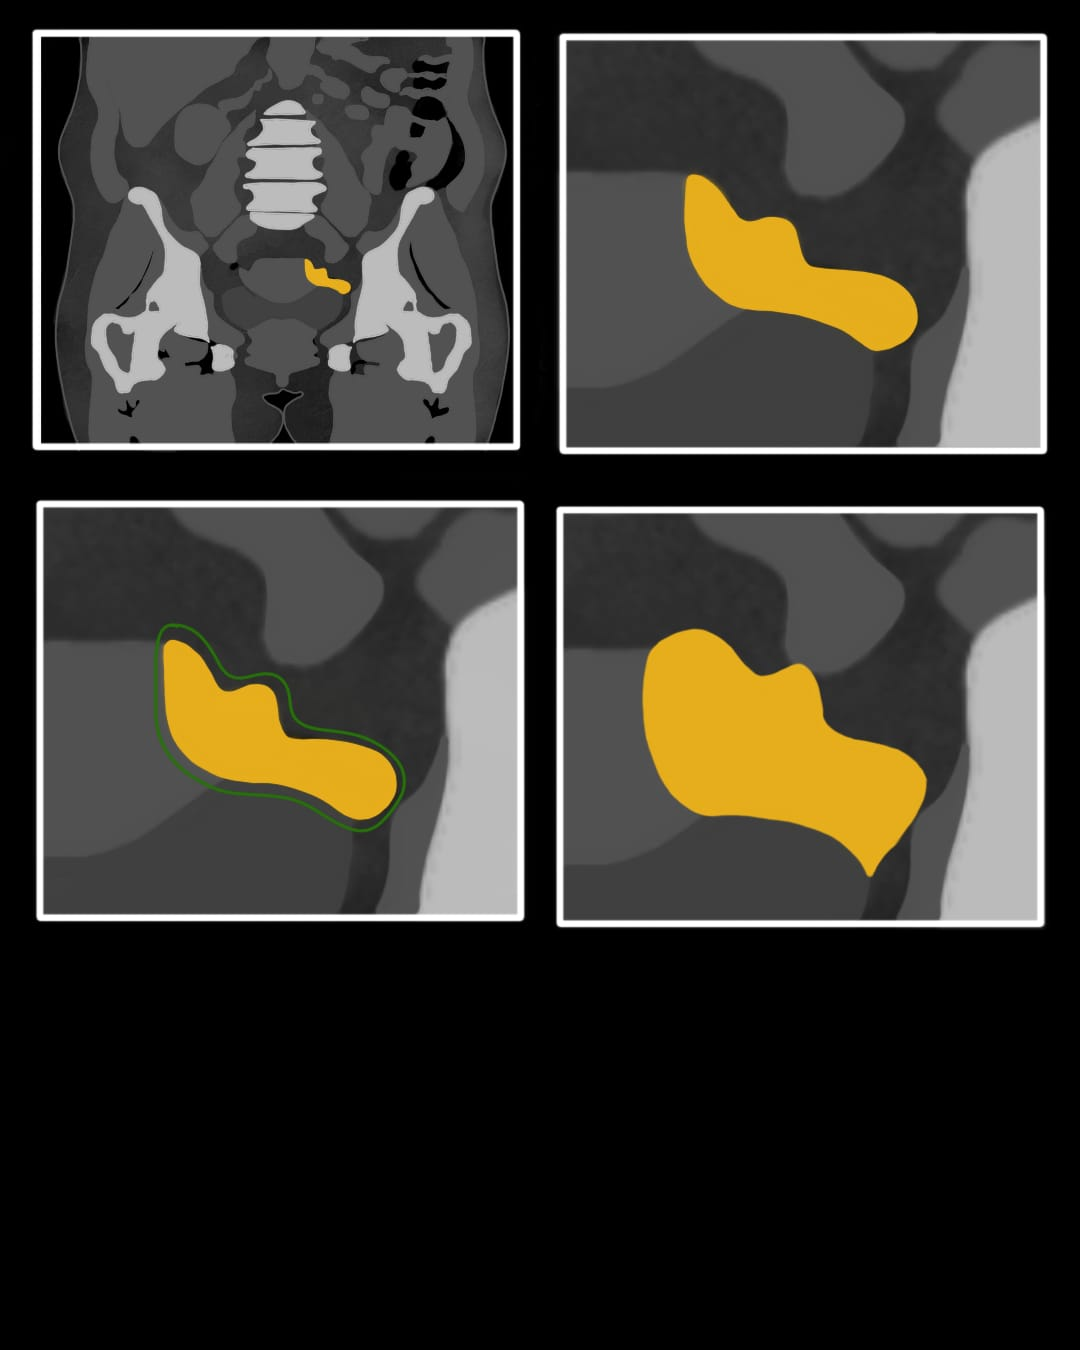
\includegraphics[width=.23\linewidth, trim=35 905 562 40, clip]{../figures/planning-areas.jpeg}\label{fig:gtv}
  }
  \subfigure[GTV macroscopic]{
    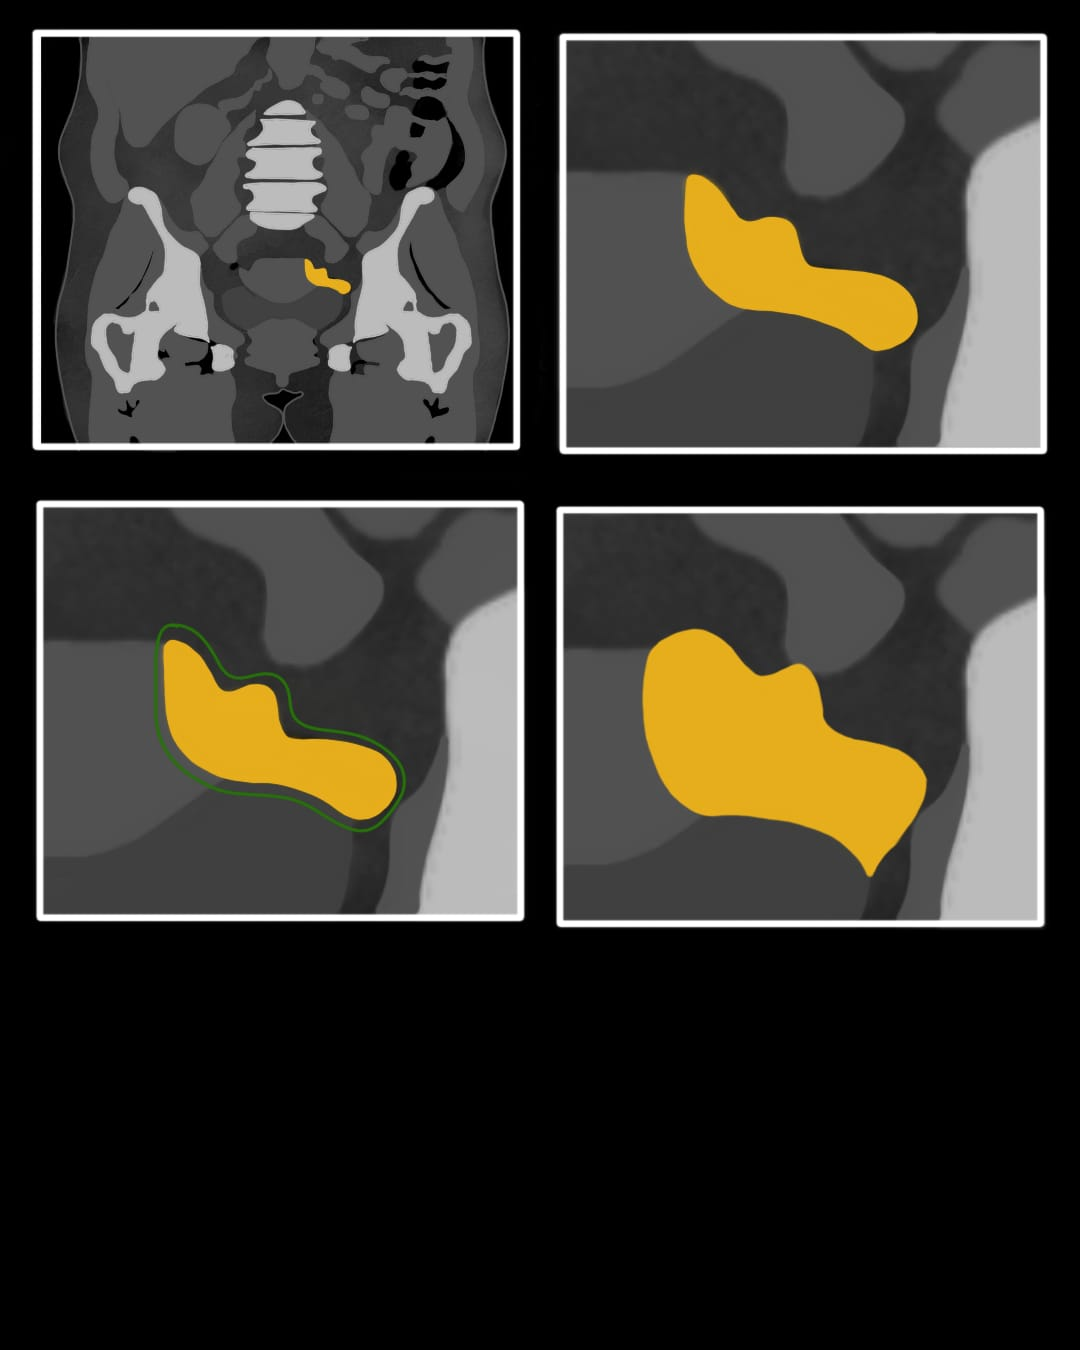
\includegraphics[width=.23\linewidth, trim=562 905 35 40, clip]{../figures/planning-areas.jpeg}\label{fig:gtv-macroscopic}
  }
  \subfigure[CTV microscopic]{
    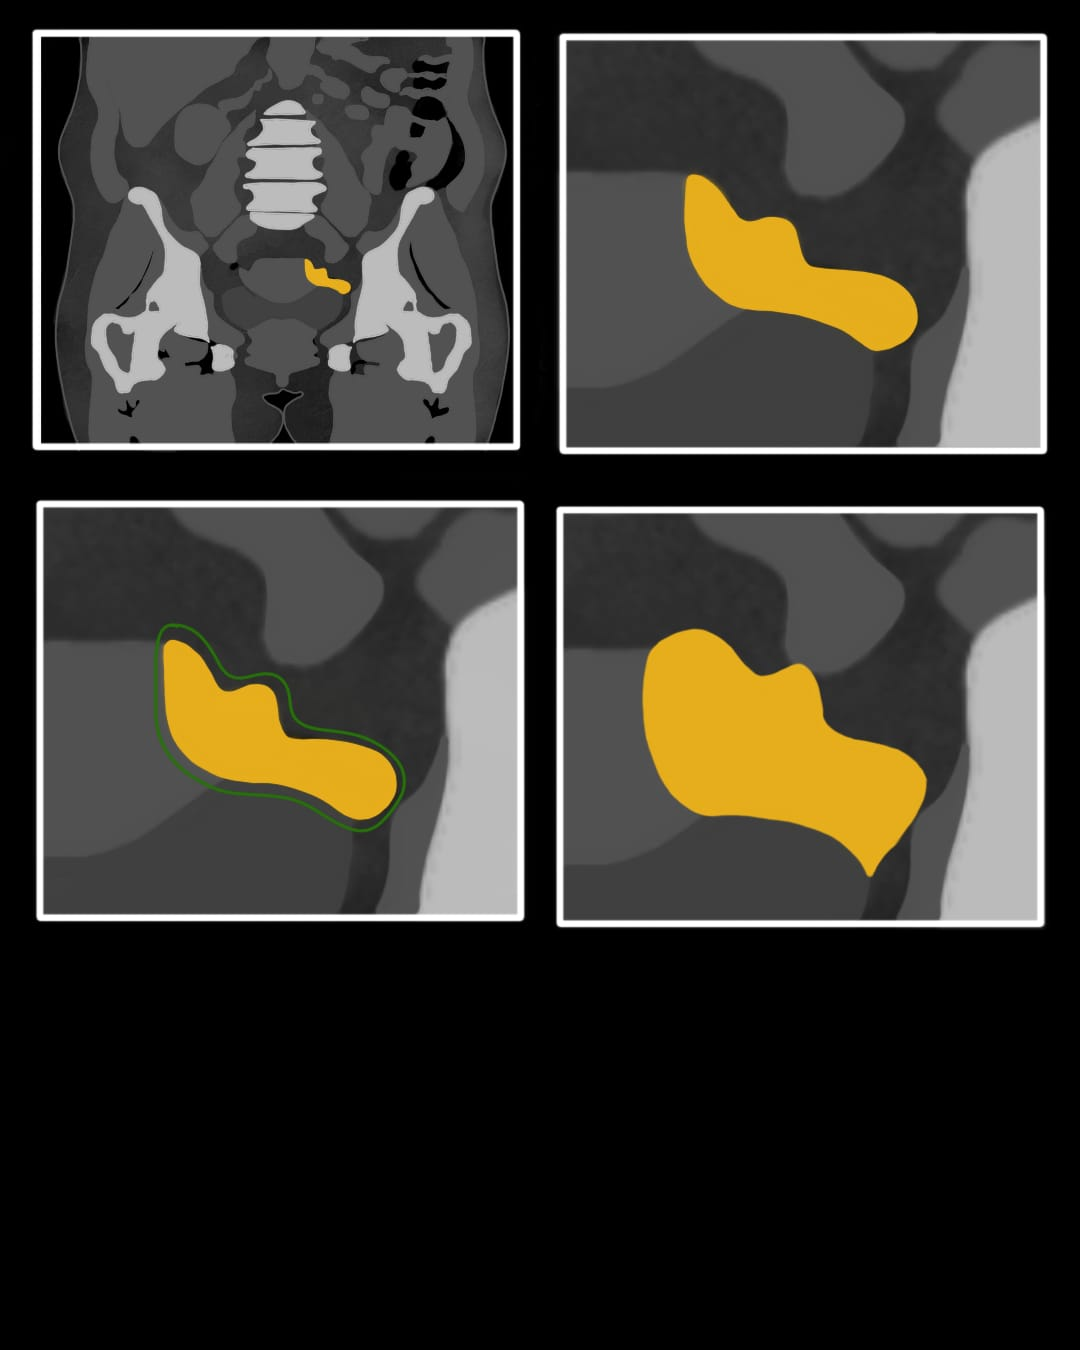
\includegraphics[width=.23\linewidth, trim=45 443 562 510, clip]{../figures/planning-areas.jpeg}\label{fig:ctv-microscopic}
  }
  \subfigure[PTV area]{
    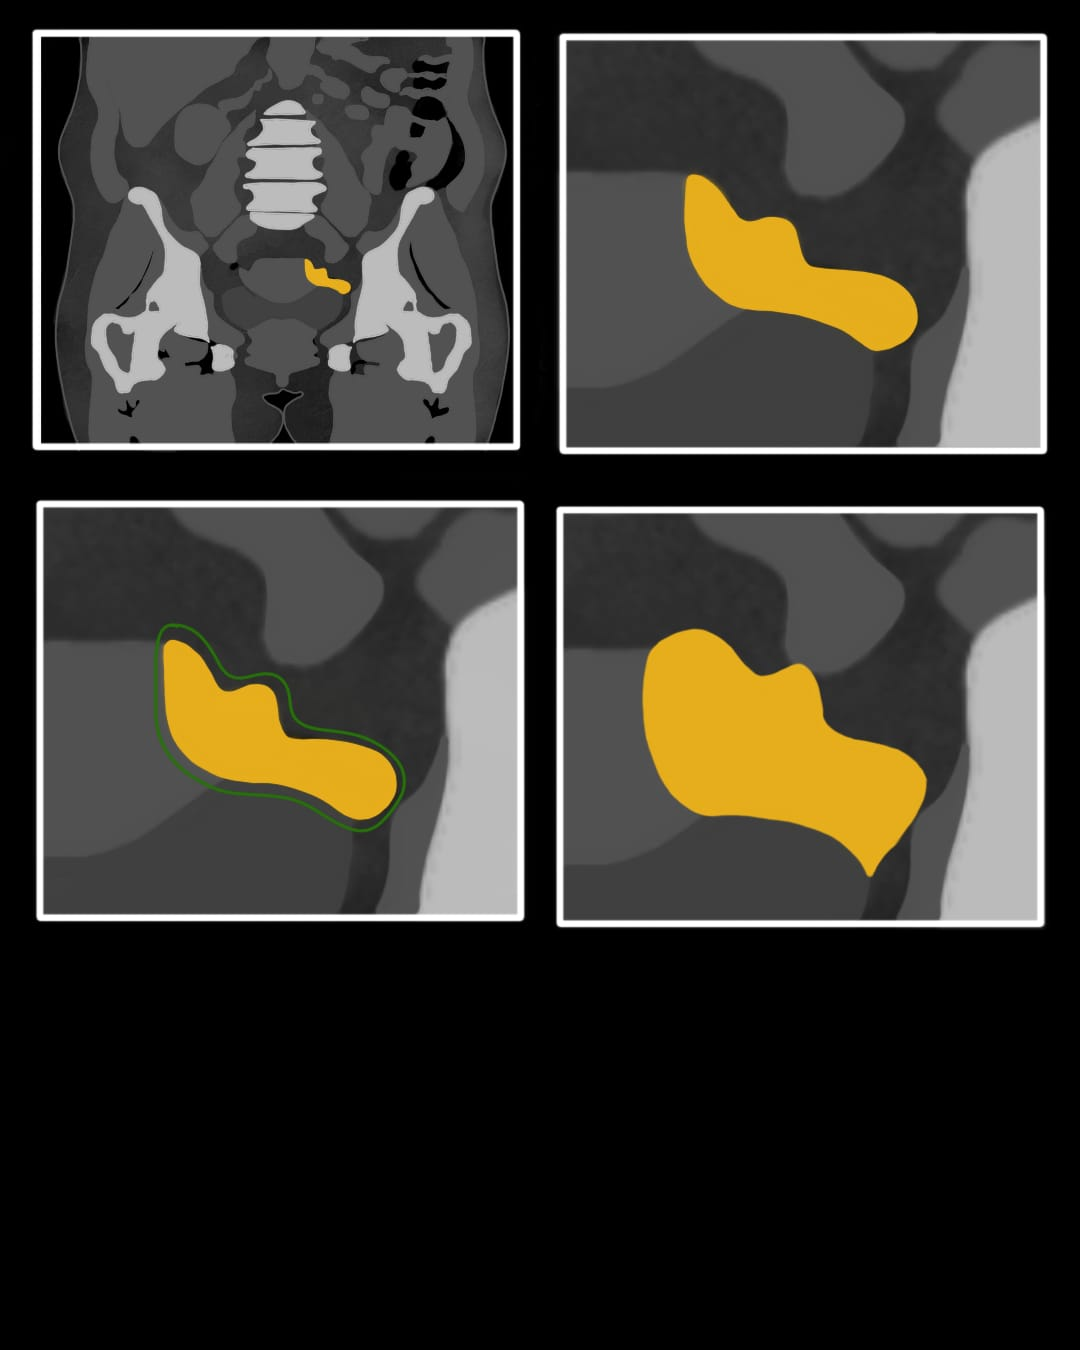
\includegraphics[width=.23\linewidth, trim=562 443 48 510, clip]{../figures/planning-areas.jpeg}\label{fig:ptv-area}
  }
  \caption{Simplified representation of the clinical target volumes. Figure~\ref{fig:gtv-macroscopic} shows the visible tumor, Figure~\ref{fig:ctv-microscopic} shows microscopic spread of the tumor, Figure~\ref{fig:ptv-area} shows area to account for short-term organ misalignment.}\label{fig:planning-areas}
\end{figure}

Oncologists use CT scans to draw clinical volumes by combining their knowledge about the particular cancer to determine target structures, organs-at-risk structures, and areas where the cancer will likely spread to~\cite{AMLART-data}. We provide a simplified representation in Figure~\ref{fig:planning-areas}.

\subsubsection{Target Volumes}

The first area is the macroscopic delineated area of the visible tumour area. This Gross Target Volume (GTV) has a high probability of containing the tumour. Secondly, the Clinical Target Volume (CTV) is derived to account for potential microscopic spread. The CTV will be an area at least as big as the GTV with an optional margin surrounding it containing a 'rind' of non-zero probability of tumour spread. Lastly, the Primary Target Volume (PTV) contains residual geometric uncertainties and safety margins surrounding the CTV, ensuring the radiotherapy dose gets delivered to the CTV~\cite{tumor-delineation,defining-target-volumes,Lin2021-oz,personalised-PTV-strategies}. The PTV is a necessary extension of the CTV since geometric uncertainties are impossible and not advised to eliminate; after all, static scans are only estimations, subject to short-term organ misalignment, relative movement between structures of reference and tumours, partial volume effects and skewed anisotropic resolution~\cite{VANHERK200452}.

\subsubsection{Organs at Risk}

In parallel, the oncologist constantly considers critical healthy tissue structures that need to be preserved during irradiation. These are referred to as organs-at-risk (ORs). These are organs that, despite being healthy, are substantially likely to be within the PTV. In some specific circumstances, adding a margin analogous to the PTV margin around an OR is necessary to ensure that the organ cannot receive a higher-than-safe dose; this gives a planning OR volume~\cite{defining-target-volumes}.

\subsubsection{International Guidelines}

The final volumes have no internationally agreed-upon guidelines, which leaves it up to the interpretation of the oncologists and Hospitals to use their heuristics when drawing areas.  This time-consuming process has high variability, causing it to suffer significantly from inter and intra-observer variability~\cite{Lin2021-oz}. 

\subsection{Data Acquisition}

The Royal Marsden Hospital provides the dataset as a set of `Neuroimaging Informatics Technology Initiative' files (NIfTI)~\cite{file-formats}. It is a lightweight alternative to other formats such as Digital Imaging and Communications in Medicine (DICOM)~\cite{file-formats} and eliminates ambiguity from spatial orientation information~\cite{dicom-to-nifti-conversion}. Libraries exist for handling these files, such as SimpleITK~\cite{SimpleITK-paper}, which we use to read and manipulate the data in this project. % The library reads, manipulates, and handles the image as a set of points in a grid occupying a physical region in space defined by the metadata to remove ambiguity from the origin, size, spacing, and so on that might vary between patient scans.

The training data provides 100 female patients that have been diagnosed with similar types of cervical cancer. Each patient comes with seven relevant segmentation classes which contribute to radiotherapy planning for cervical cancer. For reproducibility, all delineated anatomies were labelled consistently by the oncologists to improve chances that an AI model can learn cervical cancer patterns~\cite{AMLART-data}. 

% Finally, the dataset comes with ten held-out data items, which are patients with only the raw CT scan information without labels.

% \subsubsection{Notes}

% Some notes contain clinical observations about each of the 100 labelled data pairs~\cite{AMLART-data}. This small sample size of patients is also a good representation of the variability of data in the population. Because of the relatively small sample size, it is essential to be more acutely aware of the variability in the data.

% A common observation is that scans contain poor contrast. For patient 13, the note reads ``no contrast - hard to see LNs,'' which is information crucial to determining segmenting the Clinical Target Volume for Lymph Nodes (CTVn). Patients 9, 60, and 62 also have ``very large tumours''; sometimes, these even shift into uncommon areas, with ``sigmoid hanging into parametrium''. % GTV not visible?

% The notes help identify and diagnose some reasons for the model's poor performance in some cases, which may be due to the high variability between patients in quality and physiology.

\subsection{Delineation classes}\label{sect:delineation-classes}

The clinicians at the Royal Marsden Hospital have provided segmentation labels for seven high-priority regions of interest (ROI). These are the anorectum, bladder, CTVn, CTVp, parametrium, uterus, and vagina. The function of these anatomies is irrelevant to this project and is left to the reader to research further at their own discression. A high-level overview table and illustration has been supplied to provide important clinical context surrounding the anatomies [\ref{fig:delineation-classes}].

\begin{landscape}
  \begin{table}[h!]
    \centering
    \begin{tabularx}{\linewidth}{l l l l X}
      \toprule
      \textbf{Anatomy} & \textbf{Type} & \textbf{Fig} & \textbf{Equ} & \textbf{Details} \\
      \midrule
      % \textit{Illustration available at Figure~\ref{fig:example-anorectum-axial}-\ref{fig:example-anorectum-sagittal}}
      Anorectum & OR & \ref{fig:example-anorectum} & \ref{eq:ctvn-ctvp-anorectum}, \ref{eq:parametrium} & The conjoined muscles from around the rectum with susceptible nerve and blood vessels. \\
      \midrule
      % \textit{Illustration available at Figure~\ref{fig:example-bladder-axial}-\ref{fig:example-bladder-sagittal}}
      Bladder & OR & \ref{fig:example-bladder}  & \ref{eq:parametrium}, \ref{eq:bladder-ctvn} & The bladder is susceptible to urinary incontinence, infection, or impaired bladder control. \\
      \midrule     
      % \textit{Illustration available at Figure~\ref{fig:example-CTVp}}. 
      CTVp & CTV & \ref{fig:example-ctvp} & \ref{eq:parametrium}, \ref{eq:ctvp2} &      
      The primary CTV. This is an area comprised of areas where there may be local microscopic spread (uterus, cervix, upper vagina, primary tumour)~\cite{AMLART-data}.
      \\
      \midrule
      % \textit{Illustration available at Figure~\ref{fig:example-CTVn}}.
      CTVn & CTV & \ref{fig:example-ctvn} & \ref{eq:ctvn-ctvp-anorectum}, \ref{eq:parametrium}, \ref{eq:bladder-ctvn}, \ref{eq:ctvn-lymph} & 
      
      The nodal CTV is drawn according to the progression of the disease. It encompasses areas that may contain microscopic spread to lymph nodes and margins around pelic blood vessels~\cite{AMLART-data}.
      \\
      \midrule
      % \textit{Illustration available at Figure~\ref{fig:example-Parametrium}}.
      Parametrium & CTV & \ref{fig:example-parametrium} & \ref{eq:parametrium} & 
      
      The tissue surrounding the cervix/vagina at risk of local spread. The Parametrium is drawn as a complete structure and edited back to the level of the vagina to be included~\cite{AMLART-data}. \\
      \midrule
      % \textit{Illustration available at Figure~\ref{fig:example-uterus-axial}-~\ref{fig:example-uterus-sagittal}}.
      Uterus & CTV & \ref{fig:example-uterus} & \ref{eq:parametrium}, \ref{eq:ctvp2} & The whole Uterus with no editing back used to generate CTVp. \\
      \midrule
      %  \textit{Illustration available at Figure~\ref{fig:example-vagina-axial}-~\ref{fig:example-vagina-sagittal}}.
      Vagina & CTV & \ref{fig:example-vagina} & \ref{eq:parametrium}, \ref{eq:ctvp2} & From the whole vagina contour, slices deleted to leave either the upper 2cm of vagina, or 2cm below the tumour (contoured as 2cm from either cervix/ GTVp, whichever is lower)~\cite{AMLART-data}. \\
      \bottomrule
    \end{tabularx}
  \end{table}
  
  \begin{figure}[H]
    \centering
    \setlength{\fboxsep}{0pt} % Remove padding around the images (if any)
    \setlength{\fboxrule}{0pt} % Remove border around the images (if any)
    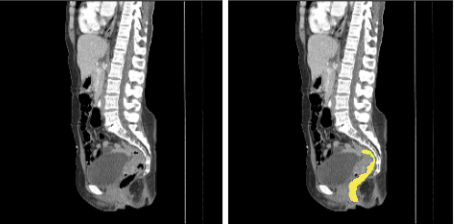
\includegraphics[width=0.14\linewidth, trim=0 0 240 0, clip]{../figures/PatientStructureExamples/Anorectum_003/51-2-266.png}%
    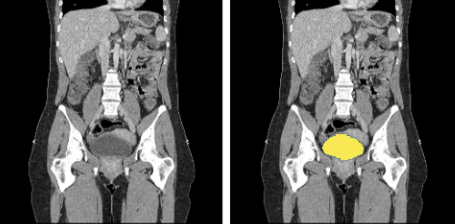
\includegraphics[width=0.14\linewidth, trim=0 0 240 0, clip]{../figures/PatientStructureExamples/Bladder_088/67-1-255.png}%
    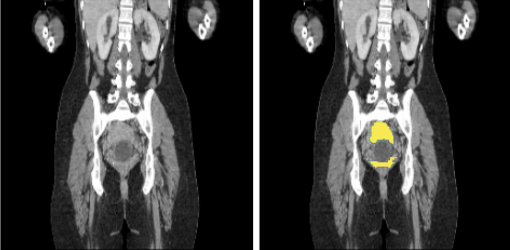
\includegraphics[width=0.14\linewidth, trim=0 0 270 0, clip]{../figures/PatientStructureExamples/CTVp_096/73-1-279.png}%
    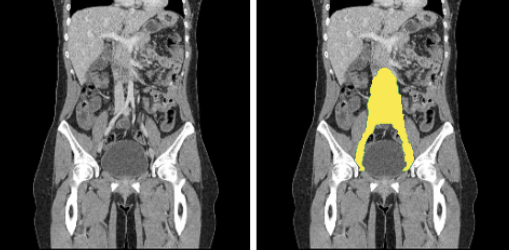
\includegraphics[width=0.14\linewidth, trim=0 0 269 0, clip]{../figures/PatientStructureExamples/CTVn_007/67-1-239.png}%
    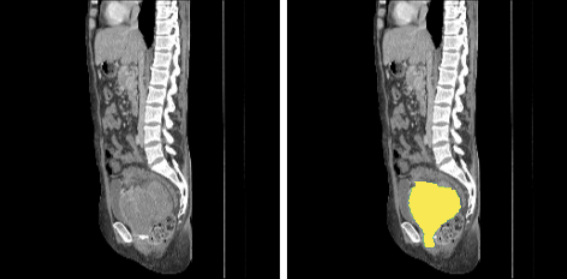
\includegraphics[width=0.14\linewidth, trim=0 0 299 0, clip]{../figures/PatientStructureExamples/Parametrium_088/9-2-234.png}%
    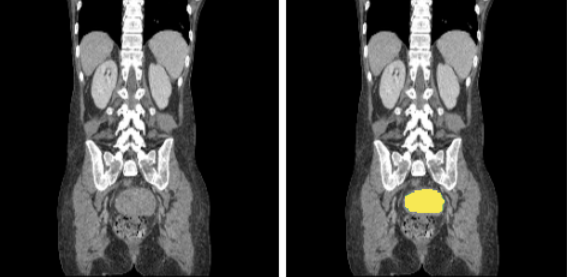
\includegraphics[width=0.14\linewidth, trim=0 0 301 0, clip]{../figures/PatientStructureExamples/Uterus_012/9-1-306.png}%
    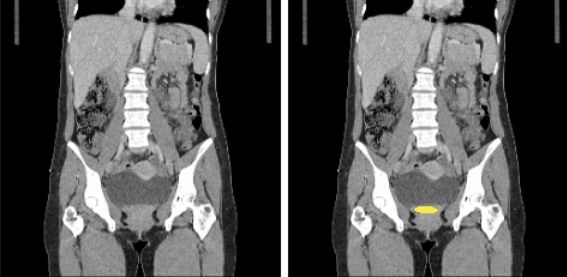
\includegraphics[width=0.14\linewidth, trim=0 0 301 0, clip]{../figures/PatientStructureExamples/Vagina_69/79-1-267.png}%
  
    \vspace{-0.5\baselineskip} % Adjust the space between rows
  
    \subfigure[Anorectum]{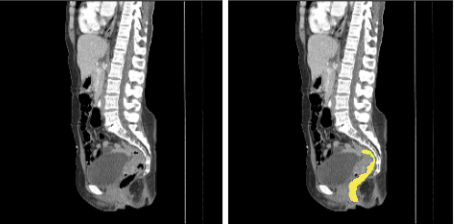
\includegraphics[width=0.14\linewidth, trim=238 0 2 0, clip]{../figures/PatientStructureExamples/Anorectum_003/51-2-266.png}\label{fig:example-anorectum}}%
    \subfigure[Bladder]{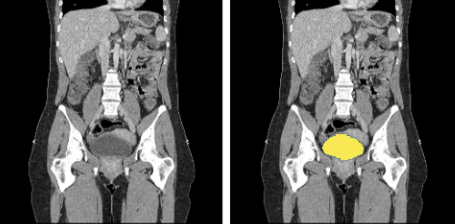
\includegraphics[width=0.14\linewidth, trim=240 0 0 0, clip]{../figures/PatientStructureExamples/Bladder_088/67-1-255.png}\label{fig:example-bladder}}%
    \subfigure[CTVp]{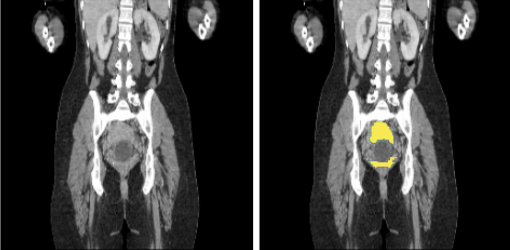
\includegraphics[width=0.14\linewidth, trim=270 0 0 0, clip]{../figures/PatientStructureExamples/CTVp_096/73-1-279.png}\label{fig:example-ctvp}}%
    \subfigure[CTVn]{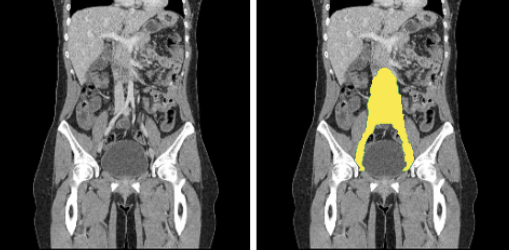
\includegraphics[width=0.14\linewidth, trim=269 0 0 0, clip]{../figures/PatientStructureExamples/CTVn_007/67-1-239.png}\label{fig:example-ctvn}}%
    \subfigure[Parametrium]{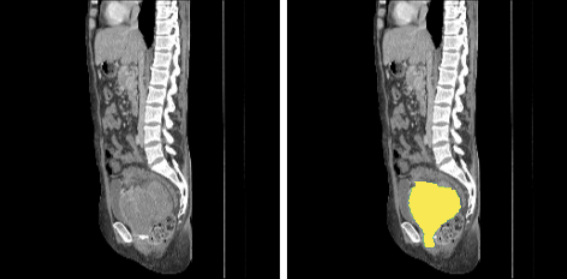
\includegraphics[width=0.14\linewidth, trim=299 0 0 0, clip]{../figures/PatientStructureExamples/Parametrium_088/9-2-234.png}\label{fig:example-parametrium}}%
    \subfigure[Uterus]{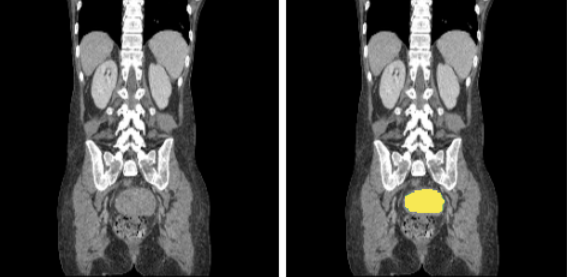
\includegraphics[width=0.14\linewidth, trim=301 0 0 0, clip]{../figures/PatientStructureExamples/Uterus_012/9-1-306.png}\label{fig:example-uterus}}%
    \subfigure[Vagina]{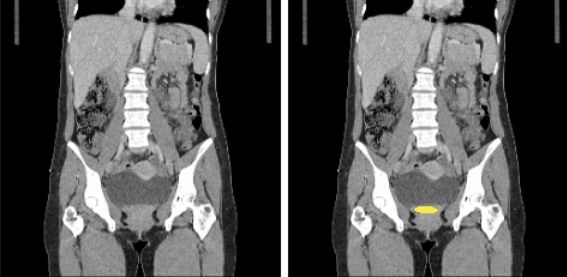
\includegraphics[width=0.14\linewidth, trim=301 0 0 0, clip]{../figures/PatientStructureExamples/Vagina_69/79-1-267.png}\label{fig:example-vagina}}
    \caption{A high-level overview of delineation classes with details regarding each if it deviates from typical objectives, e.g. see Vagina.}\label{fig:delineation-classes}
  \end{figure}

% TODO: totalsegmentator is region based, so the bladder would have been predicted in context of 24 other structures to help it guide it into the right general serach area.


\end{landscape}

\subsection{Rules}\label{sec:rules}

With the delineated areas, the clinicians outlined rules that affect the final segmentation~\cite{AMLART-data}. Note, if multiple organs are referenced, they pertain to the same patient.

Let us represent each organ anatomy as the first letter of its name, specifically: ($A$)norectum, ($B$)ladder, ($C$)ervix, ($P$)arametrium, ($U$)terus, ($V$)agina. Further, define:

\begin{enumerate}
  \item The CTVn and CTVp as $C_n$ and $C_p$ respectively
  \item The GTVn and GTVp as $G_n$ and $G_p$ respectively
  \item The Pelvic, Common and Para-aortic Lymph Node as $L_p$, $L_c$, and $L_{pa}$ respectively  
  \item The overlap of two structures is denoted by the set intersect symbol $\cap$.
  \item The joint area of two structures is denoted by the set union symbol $\cup$.
\end{enumerate}

\subsubsection{Relationship between Structures}

\begin{enumerate}
  \item There should be no overlap between the CTVn, CTVp or Anorectum.

        \begin{equation}\label{eq:ctvn-ctvp-anorectum}
          \forall{i,j \in \{C_n, C_p, A\}}\text{ with } i \neq j, i \cap j = \emptyset
        \end{equation}

  \item The Parametrium may overlap with all of the other structures.

        \begin{equation}\label{eq:parametrium}
          \forall i \in S, \quad (P \cap S \neq \emptyset) \vee (P \cap S = \emptyset), \quad \text{where } S = \{A, B, C, C_n, C_p, U, V\}
        \end{equation}

  \item The Bladder may overlap with the CTVn.

        \begin{equation}\label{eq:bladder-ctvn}
          B \cap C_n \neq \emptyset \vee B \cap C_n = \emptyset
        \end{equation}

  \item The CTVp is defined as a compound structure containing:

        \begin{equation}
          C_p = \overbrace{C \cup G_p}^{\text{High Risk CTV}} \cup \ \ U \cup V\label{eq:ctvp1}
        \end{equation}

  However, since we are never explicitly provided with the segmentation maps for the Cervix $C$ and the GTVp $G_p$, we cannot use as strong of a definition as above. Instead, we operate on the assumption that the union of the Uterus and Vagina is at least as big as the CTVp.

        \begin{equation}
          U \cup V \subseteq C_p\label{eq:ctvp2}
        \end{equation}

  \item The CTVn is defined as a compound structure containing:

        \begin{equation}\label{eq:ctvn-lymph}
          C_n = G_n \cup L_i \cup L_p \cup L_{pa}
        \end{equation}

  Similarly, we are not provided segmentations for these areas, therefore, operating under no clinical knoweldge apart from the provided, cannot make any claims as to the composition of the CTVn.

\end{enumerate}

\subsection{Motivation in AI}

The medical sector has been a hotbed for AI research since  Convolutional Neural Networks (Section~\ref{sect:image-segmentation}) have been applied on medical image data by researchers. A branch of research dedicated itself to segmentation, which involves labelling individual pixels in the image according to which object or class they belong to. In dense classification, a model assigns every pixel to a specific class. Relevant to the direction of this project is determining the precise location and extent of organs or certain types of tissue, like ORs, CTV volumes, or other anatomies. 

The key objective of models trained for delineating target structures for this project is to see if an AI model can learn cervical cancer CTV pattern detection. The decision is complex as clinicians use information beyond the CT-imaging modality, such as how far along the tumour has progressed, and other clinical intuition to make proper judgements about the CTV volumes. Therefore, with this information missing from AI models, it is likely to misjudge target volumes, and a clinician will have to select which components of the CTV are required. However, a clinician will benefit from the time saved and improved consistency with the planning process if a trained model can produce the substructures required within the CTV that a clinician can review~\cite{AMLART-data}.

\section{Machine learning for image segmentation}\label{sect:machine-learning-for-image-segmentation}

Before the popularization of machine learning, algorithms used to be defined by strict and convoluted rules. These heuristically defined algorithms struggled to scale to complex problems and were often complicated or confusing to maintain because the typical task does not warp easily into human intuition.

\begin{figure}[H]
  \centering
  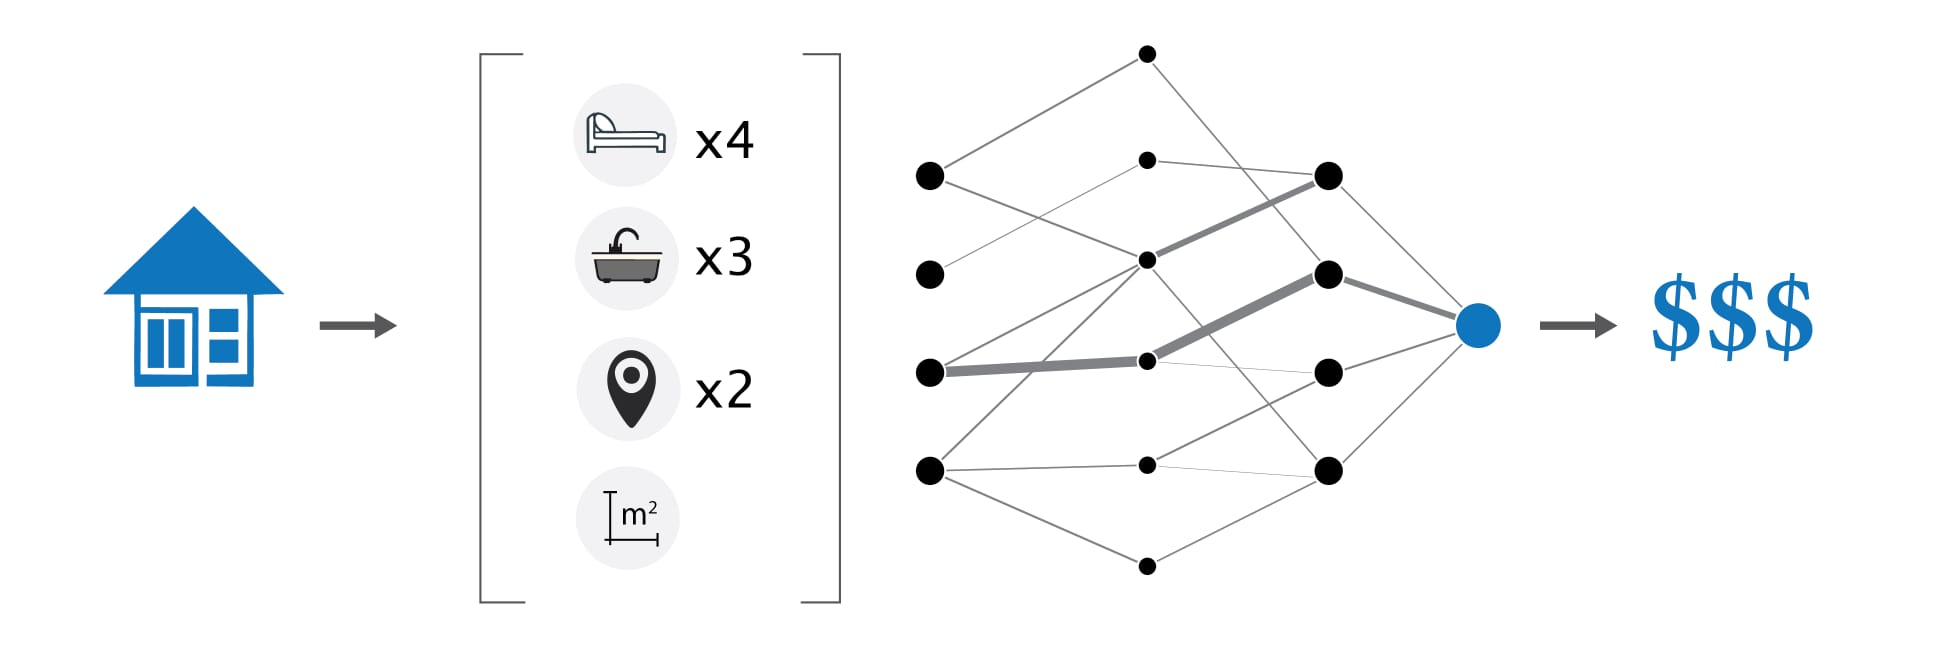
\includegraphics[width=.7\linewidth]{../figures/california.jpeg}
  \caption{An illustration of a multi-layered perceptron (MLP) for the California Housing dataset. Information is vectorised and fed into a network. Different weights/strengths are learnt for each feature. Ultimately, the model learns a relationship between the features and the target.}\label{fig:california-housing}
\end{figure}

Due to poor scalability, a new genre of algorithms emerged that fell into the classification of neural network models. Observations were rephrased and morphed into vectorised inputs, where each constituent of the vector represented a particular feature of the observation. For instance, the California Housing dataset~\cite{kelleypace1997} contains an input of 9 features (number of bedrooms, number of toilets, longitude, latitude, square footage, \dots) and one target feature (house price). After pre-processing and strategising, this input would be vectorised and fed into a network with several layers. Within each layer, sets of tunable parameters would optionally change the number of features and learn a relationship between parameters using weights until the $1 \times 9$ vector finally translates into a scalar value indicating the house price -- a simplified illustration of the process is shown in Figure~\ref{fig:california-housing}. After many repetitions of learning from examples, the model would learn an approximation to the complex objective. These models were termed Multi-Layered Perceptrons (MLPs).

\subsection{Image Segmentation}\label{sect:image-segmentation}

The current machine learning approach didn't work well with image data. Up until that point, rich structures such as images were neglected, and matrices of gray-scale images were mutilated into flat vectors. This approach was necessary to feed the flattened image representation through the MLP. The issue with vectorising an image is that it loses its spatial context-driven awareness. 

At the same time, J. Hull, sponsored by the United States Postal Service, published a Database for Handwritten Text Recognition with the incentive of providing an extensive dataset of images of characters of variable writing mediums, isolation, overlap, and neatness to aid research efforts in developing accurate digit classification algorithms~\cite{JJHull1994}. Yann LeCunn et al.~\cite{Lenet1998} used this database to propose the first Convolutional Neural Network (CNN) for image processing, which preserved the input in its 2D glory by applying convolutions. The fundamental Convolutional Filter is displayed in Figure~\ref{fig:sobel}.

\begin{figure}[H]
  \centering
  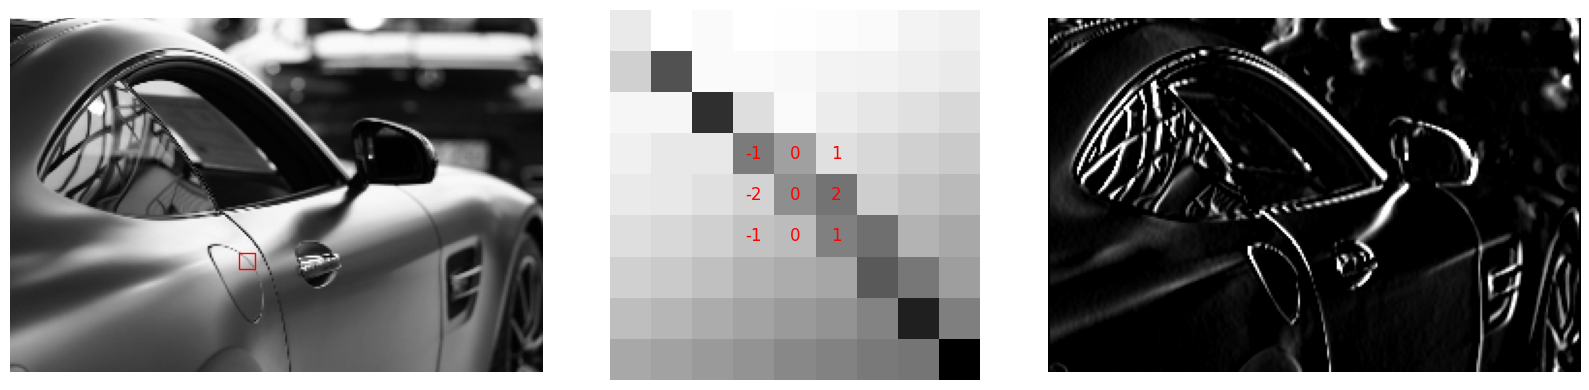
\includegraphics[width=1\linewidth]{../figures/sobel.png}
  \caption{Example application of a convolution. From left to right, the input image with a region outlined in a red box, the boxed region magnified with a convolutional (Sobel) filter being applied to a part of the magnified region, and lastly the output after the filter has passed over the entire image. The output represents a new feature map encoding features of the original (input) feature.}\label{fig:sobel}
\end{figure}

Convolutional layers are rectangular blocks that are recipes for translating an image (alternatively known as the input feature). The algorithm centres the block over a specific pixel and uses a square radius of neighbouring pixels. It multiplies and sums the pixels along the corresponding pixel positions according to the recipe to produce a transformed resulting pixel that encodes the reference pixel's information and the surrounding receptive field around it. Figure~\ref{fig:sobel} demonstrates this concept. Specifically the middle tile, which shows an example $3 \times 3$ convolutional filter being applied to a zoomed in part of the image. This filter slides across the entire image and encodes it which produces the output on the right of Figure~\ref{fig:sobel}. 

The CNN operates by having multiple learnable convolutional filters stacked on top of each other. The values within the square convolutional filter are \textit{learned} during training; the values learnt are those that, in combination with the layers before and after, encode the image's features according to the training objective the best. When stacked with many other convolutional filters that piggyback off the encoded features produced by filters before it, this allows for dense feature representations that encode the entire image.


This first convolutional network spawned a vicious flurry of convolutional architectures, which followed in their footsteps. The Fully Connected Neural Network (FCN) adapted the architecture used by LeCunn et al.~\cite{Lenet1998} for segmentation applications. Previously, convolutions would reduce input image feature vectors into non-spatial classification outputs. However, this paper `convolutionalized' the pipeline to provide a heatmap of segmented objects within the image~\cite{fully-CNNs-for-semantic-segmentation}. The heatmap would describe in a 2D feature the location of each class.

\begin{figure}[H]
  \centering
  \subfigure{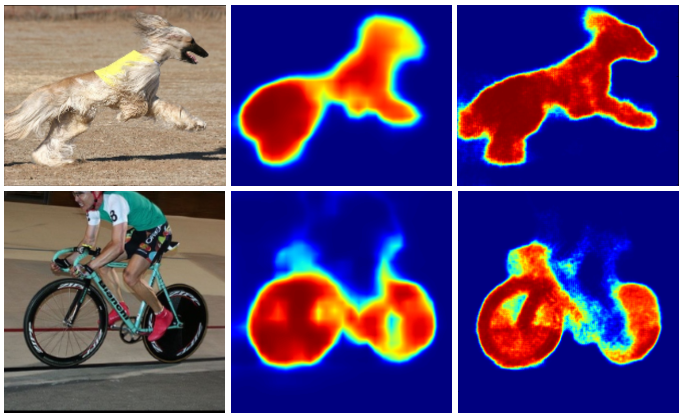
\includegraphics[width=.49\linewidth, trim=0 230px 0 0, clip]{../figures/fcnupsample.png}}
  \subfigure{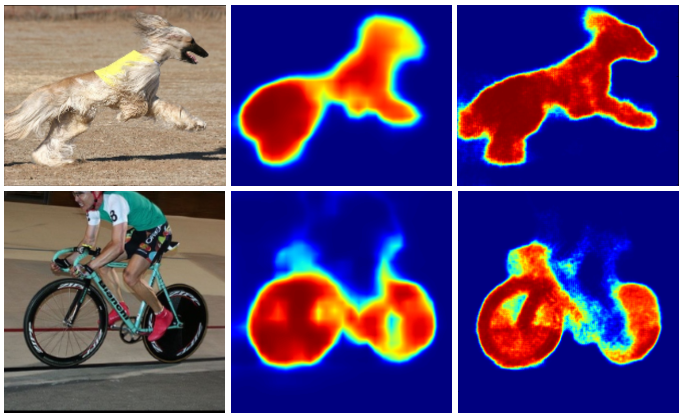
\includegraphics[width=.49\linewidth, trim=0 33px 0 200px, clip]{../figures/fcnupsample.png}}
  \caption{Comparison of upsampling a base image using FCN~\cite{fully-CNNs-for-semantic-segmentation} and the VGG-16-based DeconvNet~\cite{noh2015learning, simonyan2014very} architectures.}\label{fig:fcn-vs-deconvnet}
\end{figure}

% TODO: maybe a bit more context surrounding VGG

Trivial upsampling through de-convolutional layers allows the heatmap to translate back to the original size. This process would produce a largely inaccurate segmentation with much room for improvement. Therefore, similarly to learning the downsampling, the model learnt to upsample low-level heatmap representations~\cite{noh2015learning}. This way, the deconvolutional network also became ``a key component for precise object segmentation'', which improved the base upsampling provided by the FCN. This conclusion is shown in Figure~\ref{fig:fcn-vs-deconvnet}.

The strategy of downsampling and upsampling for image segmentation is a common theme amongst many segmentation architectures.

\subsection{U-Net}

\begin{figure}[H]
  \centering
  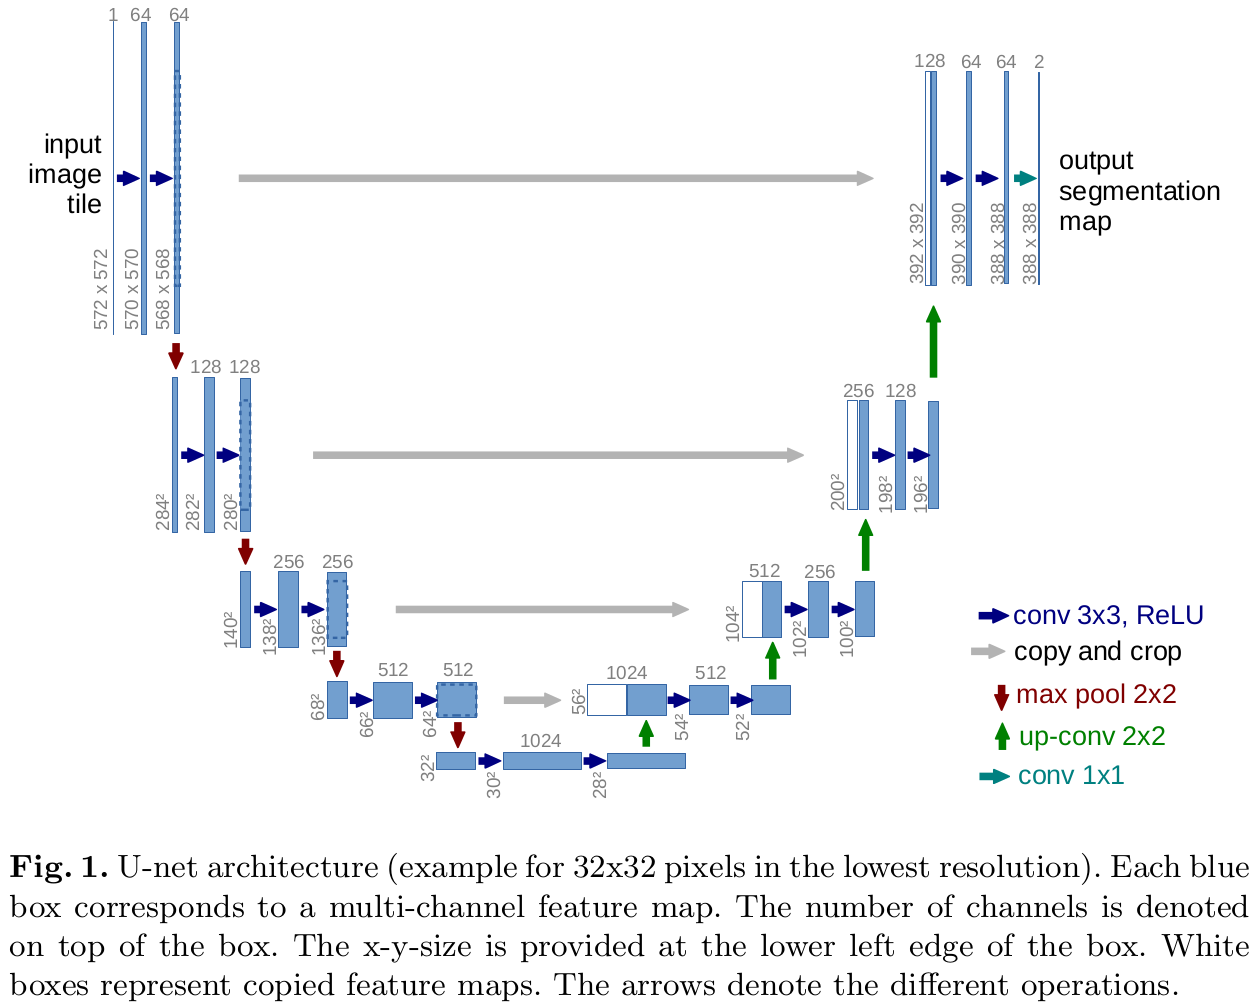
\includegraphics[width=.8\linewidth, trim=0 200px 0 0, clip]{../figures/u-net.png}
  \caption{The U-Net architecture, with contractive side on the left, and expansive side on the right. The feature map follows the arrows and multiplies the number of feature maps twice at each contraction, and halves at each expansion~\cite{U-Net}.}\label{fig:unet}
\end{figure}


Simultaneously, a unique architecture was under development. This architecture mirrored the hourglass structure of contracting and upsampling sections of the FCN, only this time, the illustration of its architecture led to its name, the U-Net~\cite{U-Net}.

The U-Net similarly consists of a contractive and expansive side, with the added feature of so-called `skip-connections'. As shown in Figure~\ref{fig:unet}, at each stage of the contracting/expansive side, these copy operations help localise high-resolution features from the contracting path~\cite{U-Net}. The network yielded great results for a few training images and more precise segmentations.

% TODO: skip connections glue the output of previous layer on

The U-Net was now very close to being a staple choice in biomedical data for anatomy segmentation. A limitation of its current implementation is that slices along the third dimension would most certainly contain contextual information that would influence the decision of the current design. Therefore, an identical network topology with extended 3D convolutions was proposed by \c{C}i{\c{c}}ek et al.~\cite{DBLP:journals/corr/CicekALBR16}.

\subsection{nnUNet}\label{sect:nnunet}

The nnUNet is closely related to the U-Net architecture. However, nnUNet's ability to adapt to the data improves this model performance over the vanilla implementation.

Until now, architectures have operated on data pre-processed to a particular expected distribution and configured to deal with a specific problem. For instance, out-of-the-box configuration has stringent input size requirements, which require image resizing. Furthermore, 3D images commonly produce heterogeneous voxel spacing depending on the parameters chosen by the clinician or the machine from which they were produced~\cite{nnunet}. The number of moving parts often leaves a unidirectional dependency on the data depending on the architecture. 

\subsubsection{Automated Method Configuration}\label{sect:nnunet-automated-method-configuration}

Therefore, the nnUNet analyses the fingerprint of the dataset and the device to deliver a tailored experience and force a more codependent relationship; now, the architecture depends on the data and the data is pre-processed to conform to the network~\cite{nnunet}. Furthermore, hardware restrictions mean networks may be inaccessible to those with worse specifications or, at the other end of the spectrum, may underutilize powerful computation still available~\cite{nnunet}; the nnUNet analyses GPU constraints used to influence batch sizes and more~\cite{nnunet-git-paper}.

The automated method configuration is classified into three categories. A dataset fingerprint extracts training data distributions such as shape, spacing and intensity distributions. Rule-based parameters estimate the most common robust parameters for resampling and normalization. Finally, the Empirical Parameters learn parameters, such as ensemble selection, which is not derivable from the dataset fingerprint.

\subsubsection{Critical Review of the nnUNet}

A review of segmentation methods in 2024 reviewed some further developments in segmentation models and found that the convolution-based U-Net architectures continued to outperform Attention-based or Mamba-based approaches six years after the initial publication of the self-configuring network~\cite{isensee2024nnunet}. Isensee et al. concluded that there was a significant mischaracterisation of proclaimed improvements in new strategies such as transformers. Claims of performance improvements over the nnUNet were reviewed through the control of validation datasets and removals of baseline tampering, which demonstrated the convolution-based performance on datasets with low statistical intra-method standard deviation~\cite{isensee2024nnunet}.

The continued performance dominance gives the nnUNet a good foundation for being used as a baseline model for all datasets.

\subsection{TotalSegmentator}

TotalSegmentator is a tool based around the nnUNet. TotalSegmentator is pre-trained on 1204 CT examinations to provide plans to segment 104 anatomical structures. The anatomies selected included apparent structures such as skeletal structures, gastrointestinal organs and other major organs. The training data contained many CT images, with differences in slice thickness, resolution, and contrast phase~\cite{totalsegmentor-paper}. However, it is important to note that 60\% of the scans occurred in a contrast-enhanced environment, which plays a role in how obvious delineations are during scanning, a scanning detail that was omitted during the training data collection for this research project. Furthermore, only an estimated 10\% of the data collected from this model contained relevant studies for the abdomen and pelvic areas.

From the segmented organs that total segmentator provides, only the Bladder overlapped with the organs that were of interest in this study.

\subsection{UniverSeg}\label{sect:universeg}

Convolutional architectures like those discussed above utilize many-shot learning (Section~\ref{sect:many-shot-learning}). However, models trained on segmenting a target domain (e.g., bone delineation) do not transfer to other domains (e.g., organ segmentation) without fine-tuning.

\begin{figure}[H]
  \centering
  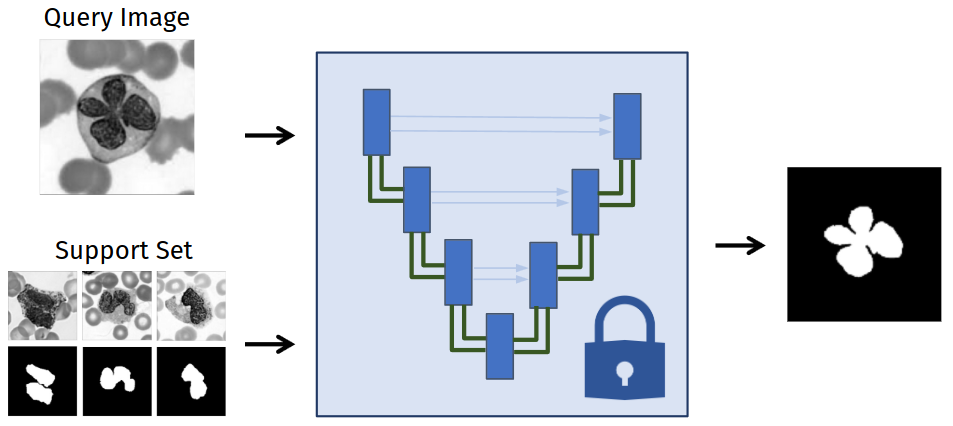
\includegraphics[width=.5\linewidth]{../figures/universeg.png}
  \caption{The UniverSeg architecture~\cite{universeg}. Diagram illustrates the freezing of model parameters while providing a support set of images which follows the query image through the segmentation pipeline.}\label{fig:universeg}
\end{figure}

Butoi et al. present UniverSeg, a model that breaks away from the traditional approach; instead of training a model on a single task (e.g. bone delineation) and freezing parameters during inference, this architecture uses a support set of images to provide a practical few-shot approach to inferring segmentations from input images. Figure~\ref{fig:universeg} shows an example of this efficient querying, which manifests itself in a U-Net architecture where the support set passes through the network along the query to influence the final segmentation. This way, Butoi et al. attempt to provide segmentation on a target image based on examples of other samples with the same anatomy contoured in a selection of other images. Therefore, the model can learn to segment both bone and organ segmentation tasks without the need for fine-tuning~\cite{universeg}.

This model operates on 2D slices of images and directly avoids the finetuning argument for medical imaging. They argue that finetuning can be unhelpful due to the differences between medical domains, features, and data fingerprints. As such, UniverSeg avoids significant retaining for each subtask.

% Fully transferable, no retraining, few shot learning

% This is especially problematic in the medical domain where clinical researchers or other scientists are constantly defining new segmentation tasks driven by evolving populations, and scientific and clinical goals. To solve these problems they need to either train models from scratch or fine-tune existing models.

% Fine-tuning models trained on the natural image domain can be unhelpful in the medical domain [ 82 ], likely due to the differences in data sizes, features, and task specifications between domains, and importantly still requires substantial retraining. 

% Universeg avoids substatial retraining for each subtask

\subsection{SAM}\label{sect:sam}

\begin{figure}[H]
  \centering
  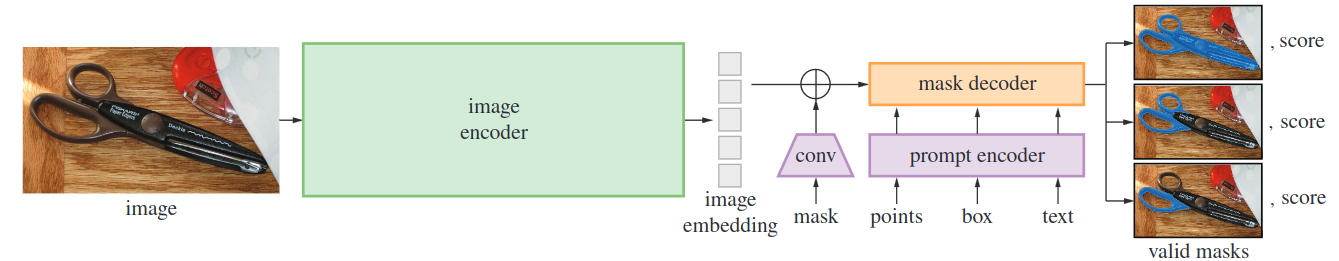
\includegraphics[width=1\linewidth]{../figures/SAM.png}
  \caption{The SAM model involves a transformer architecture that embeds points and bounding boxes into a promptable encoding, which is used in tandem with the image encoding to produce the most likely segmentation of the described area~\cite{SAM}.}\label{fig:sam}
\end{figure}

Advances in NLP, with attention-based mechanisms, have questioned whether convolutional-based methods like those above are the best approach for segmentation. Transformers from NLP were adapted to form the Vision Transformer (ViT)~\cite{ViT}. This model views the image as a grid of tokens; in the original paper, Dosovitskiy et al. separate the image into a grid of patches and read in these grid cells as individual tokens. The tokens pass through the attention mechanism as with NLP and into a classification mechanism~\cite{ViT}. 

% TODO search and replace normalize -> normalise
The SAM (Segment Anything Model) model implemented a modification of the transformer architecture~\cite{SAM} as seen in Figure~\ref{fig:sam}. However, the task was reformulated as a promotable segmentation problem to allow for zero-shot generalisation (the model can generalise to unseen examples with no re-training or fine-tuning). As seen in Figure~\ref{fig:sam}, the model inputs an image along with either points in the image or boxes. This reduces the search space SAM has to perform to segment an object into an area or a set of points.

\subsection{MedSAM}\label{sect:medsam}

\begin{figure}[H]
  \centering
  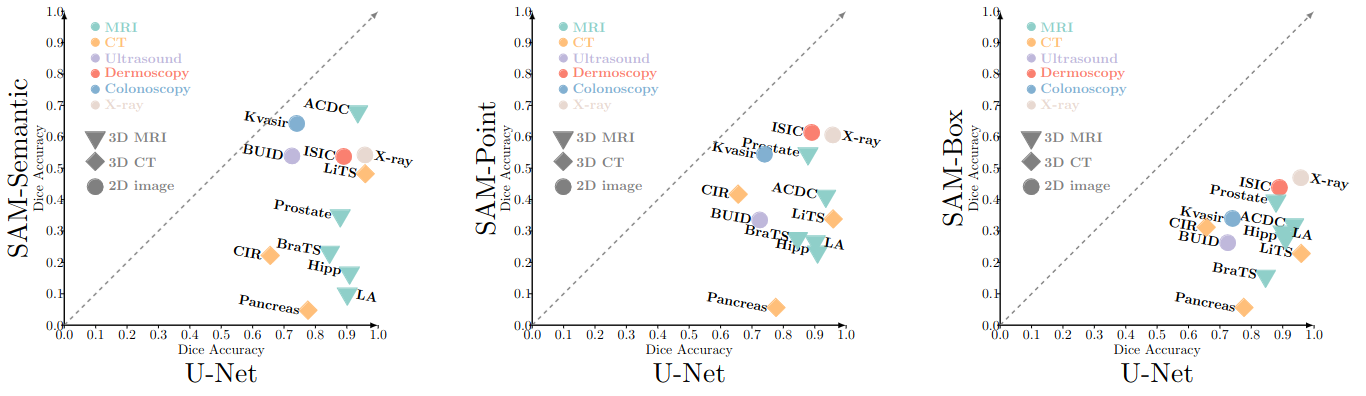
\includegraphics[width=1\linewidth]{../figures/sam-performance.png}
  \caption{Performance of a SAM model across a reference nnUNet baseline when applied to different datasets. The evaluation was considered for semantic, point and box prompts.~\cite{he2023computervision}.}\label{fig:sam-performance}
\end{figure}

SAM trains its network on a collection of natural images, not medical images such as CT and MRI scans. Extensive stress tests performed on SAM concluded that SAM's out-of-the-box promotable segmentation tool had good baseline performance on large visible objects~\cite{deng2023segment} but required exact prompt segmentation, making it inaccessible to automated contouring. Regarding the number of points required to make a sensible prediction, SAM quantitatively underperformed a nnUNet baseline, with qualitative evaluation showing fuzzy boundaries in medical contexts~\cite{hu2023sam}. Finally, Figure~\ref{fig:sam-performance} shows the performance of SAM against an nnUNet baseline across a set of datasets and imaging modalities~\cite{he2023computervision} which concludes that SAM never outperformed the nnUNet baseline when trained on the 11M natural images~\cite{SAM}. 

Therefore, Ma et al. enhanced the architecture provided by SAM by training it on a dataset of nearly 500k CT scan test examples to train a model for medical images, named MedSAM~\cite{Ma2024}. Ma et al. decided to keep close to its original despite medical images being 3-dimensional in CT and MRI scans because of ``enhanced flexibility and adaptability'' where slices along an axis substitute 3D scans~\cite{Ma2024}. This model demonstrates an improvement over SAM, nnUNet, and Deepmedic models when MedSAM bounding boxes extracted from the ground truth prompt the model~\cite{Ma2024}.

\section{Transfer Learning}

Transfer Learning involves using a model trained on a large dataset. The pre-trained model serves as the starting point for a second task where data acquisition is limited or improbable. Transfer learning is successful because, in the early layers of a model, it typically learns very low-level features. At this scale, the objective of the original domain does not matter; regardless of the initialisation, a model working on a similar problem will inevitably learn similar low-level features. 

Arguably, the universality of the parameters learnt in a model with prosperous access to data will have richer and better patterns that another with less data did not have enough information to learn~\cite{deep-learning-book, survey-on-transfer-learning}.

Transfer Learning has the potential to improve initial performance using only the transferred knowledge before any further learning begins, improve the time it takes to thoroughly learn the target task given the transferred knowledge, and improve the final performance all when compared to initial benchmarks without transfer~\cite{torrey-handbook}. Medical contexts have already applied Transfer Learning, which reportedly improved weight initialisation for 332 abdominal liver CT scans and resulted in faster convergence, providing a more robust representation~\cite{liver-lesion-via-transfer-learning}.

Transfer Learning has been seen to prevent overfitting in domains where data volume is low and where generality without overfitting is hard to come by. The prevention is because the model has already learnt features likely to be helpful in the second task~\cite{geeks-transfer-learning}. Overfitting may still occurr if the model is fine-tuned too much on the second task, as it may `learn task-specific features that do not generalise well to new data'~\cite{geeks-transfer-learning}.

\subsection{Mathematical Definition}

Transfer Learning can be formalised mathematically~\cite{survey-on-transfer-learning, concise-review-of-transfer-learning}.

\begin{itemize}
  \item Define the starting domain the model trains on initially as $\mathcal{D} = \{\mathcal{X}, P(X)\}$ with feature space $\mathcal{X}$ and a marginal probability distribution $P(X)$. $X$ is defined as an instance set, and $X = \{x_1, x_2, \cdots, x_n\} \in \mathcal{X}$.
  
  \item The original task attempts to predict data from domain $\mathcal{D}$ through a mapping $\mathcal{T} = \{\mathcal{Y}, f(\cdot)\}$ composed of a label space $\mathcal{Y}$ and an objective predictive function $f(\cdot)$. Given a domain $\mathcal{D} = \{\mathcal{X}, P(X)\}$ the sample data consists of pairs $\{x_i, y_i\}$ where $x_i \in X$ and $y_i \in \mathcal{Y}$. The objective function $f$ is supposed to learn from sample data to predict the corresponding label for the new instances. $f$ can be rewritten as $f(x)=P(y|x)$.
  
  \item The transfer learning task involves a source domain $\mathcal{D}_S$ with corresponding source tasks $\mathcal{T}_S$, and a target domain $\mathcal{D}_T$ with corresponding target task $\mathcal{T}_T$. The goal is to transfer the related knowledge to boost the performance of the target predictive function $f_T(\cdot)$.
\end{itemize}

\subsection{Shot based learning}

\begin{figure}[H]
  \centering
  \raisebox{-0.5\height}{
    \subfigure[Zero-shot]{
      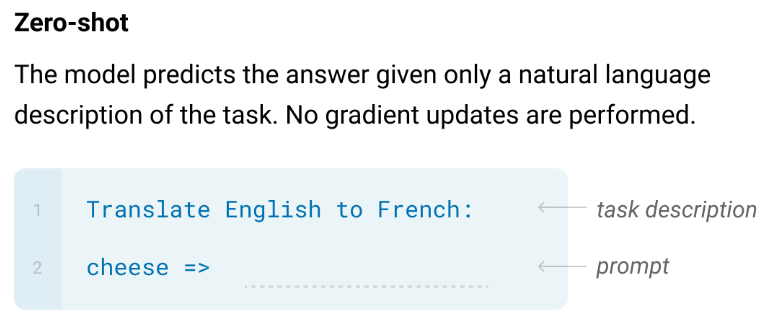
\includegraphics[width=.4\linewidth]{../figures/zero-shot-learning.png}\label{fig:zero-shot}
    }
  }
  \raisebox{-0.5\height}{
    \subfigure[Few-shot]{
      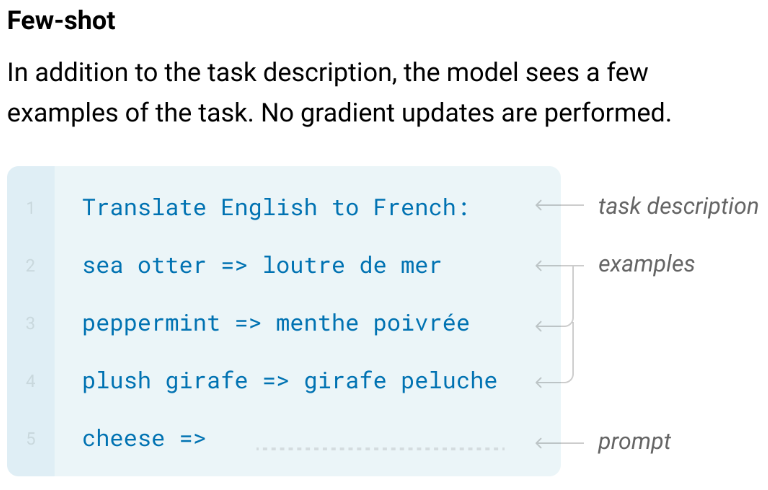
\includegraphics[width=.4\linewidth]{../figures/few-shot-learning.png}\label{fig:few-shot}
    }
  }
  \caption{Shot based learning captured in the natural language context~\cite{openaishotbasedlearning}}
\end{figure}

The transfer of models is dependent on the strategy the model uses to make predictions. Shot-based learning is a substantial factor. This describes the model's exposure to data in domains and its ability to handle cases it has never seen before. Thus, shot-based learning can be separated into meta-learning tasks or multitask learning. 

Instead of learning underlying patterns, meta-learning models learn to \textit{learn} the algorithm itself. This allows it to generalize tasks with few labelled examples of new or rare cases. Otherwise, multitask learning makes predictions for a particular set of tasks~\cite{deep-learning-book}.

\subsubsection{Zero-shot Learning}\label{sect:zero-shot-learning}

Zero-shot models (Figure~\ref{fig:zero-shot}) can generalize to unseen tasks. An example of a model targeted for zero-shot transferability is the SAM model (Section~\ref{sect:sam}).

\subsubsection{Few-shot Learning}\label{sect:few-shot-learning}

Few-shot models (Figure~\ref{fig:few-shot}) can generalize to unseen tasks with a few examples. The UniverSeg model is the target model for few-shot transferability (Section~\ref{sect:universeg}).

\subsubsection{Many-shot Learning}\label{sect:many-shot-learning}

Many-shot models can generalize to unseen tasks with many examples. The nnUNet based models such as the TotalSegmentator is the target model for many-shot transferability (Section~\ref{sect:nnunet}).

%%%%%%%%%%%%%%%%%%%%%%%%%%%%%%%%%%%%
\chapter{Methodology}\label{sect:methodology}

Improvements over the transfer from models trained on other domains could hypothetically allow the segmentation of delineated areas more accurately. To investigate this claim, we iterate over the three types of shot learning, zero-shot, few-shot, and many-shot learning, to determine the effectiveness of transfer learning in the radiotherapy domain.

\section{Transfer Strategy}

Transfer learning involves obtaining a pre-trained "base" model, identifying transfer layers, and fine-tuning the remaining layers. Key considerations include preventing overfitting on smaller datasets and making decisive adjustments to learning rates during the fine-tuning phase.

\begin{enumerate}
  \item Obtain a pre-trained ``base'' model trained on extensive data which identifies general features and patterns relevant to the target domain.
  
  \item Identify the transfer layers. These layers capture general information relevant to both the new and previous tasks. The selected layers are 'frozen' during training. This means parameters are not changed, preserving the low-level learnt feature functions. 
  
  The number of frozen layers depends on how much inheritance is required from the pre-trained model. For unrelated domains, like car vs. face detection, only low-level features should be transferred. However, the amount of information transferred in related domains is more generous, and the quantity is tunable.
  
  \item Fine-tune and retrain the remaining layers. The goal is to preserve the knowledge from the pre-training while enabling the model to modify its parameters to suit the demands of the current assignment better~\cite{geeks-transfer-learning}.
  
  For smaller datasets, there may be an issue of overfitting because the number of available samples to train on has decreased. Thus, we must set the learning rate to be low; when fine-tuning a new model you want to readjust the pre-trained weights, and if the learning rate is too high, the model may rapidly overfit~\cite{geeks-transfer-learning}. Furthermore, this is done for a low number of iterations for the same reasons~\cite{deep-learning-book}.
\end{enumerate}

\section{Baseline -- nnUNet}

The provided examples of the objective are enough to train an nnUNet model from scratch. It has been shown that in many biomedical applications, ``only very few images are required to train a network that generalises reasonably well''~\cite{DBLP:journals/corr/CicekALBR16}. Therefore, we first train a baseline nnUNet model on the provided examples to establish a benchmark for the transfer models.

\subsection{Preprocessing}\label{sec:nnunet-preprocessing}

Prior to training, necessary normalization must take place to standardize each input. Firstly, CT scans can produce results for different spacings, resolutions, and dimensions. Because the model samples data in batches, the batch properties must align within the model's body. Therefore, the fingerprint taken by the preprocessing pipeline resamples input data towards the median dimension. 

The traditional method of normalization involves normalizing the entire image corpus. However, this method does not take into account the skew that might affect the outcome. This is because the background value occurs most frequently, and artifacts such as metal cause outlier peaks. As a result, traditional normalization could overlook important tissues as it attempts to treat background and outlier values equally with foreground values.

Therefore, the nnUNet avoids this complication by processing voxel properties encased by the ground truth segmentation. The values are clipped to their 0.5 and 99.5 percentile, followed by traditional normalization with the mean and standard deviation. This way, the target structure properties remain relative to their original, and the background label conforms to the normalization inspired by the region of interest.

\subsection{Separate Training}\label{sec:train-nnunet}

The default strategy is to consider each anatomy separately and attempt to learn segmentation patterns without considering constraints mentioned in Section~\ref{sec:rules}. These models can be used in an ensemble system to produce thorough segmentations of the target volumes, oblivious to clinical constraints. 

We set up the learning pipeline to follow a five-fold cross-validation process. Each fold involves splitting the data into five subsets. Then, the model is trained on four subsets and validated on the fifth subset. The process repeats for each of the five subsets, with each subset used exactly once as the validation set. Cross-validation helps assess the model's performance and generalize it to new data. Ultimately, the model with the best validation performance represents the anatomy.

\section{TotalSegmentator}\label{sect:totalsegmentator}

TotalSegmentator uses a pre-trained nnUNet model to segment 104 anatomical structures. The model will provide insights into the performance of many-shot transfer for the Bladder and zero-shot transfer for the other anatomies. TotalSegmentator is an excellent model to use as the initial stepping stone due to its close ties with the selected binary segmentation nnUNet baseline, allowing for concrete and just conclusions about the effectiveness of transfer learning.

When transferring information, many-shot transfer is the most obvious choice. This transfer technique has the potential to increase the amount of helpful information that can be used to segment anatomies in the target domain by transferring the original task. The hypothesis is that many-shot transfer will improve segmentations for clear organ delineations. 

\subsection{Separate Training}

Like the nnUNet, we apply the default fine-tuning strategy to a pre-trained TotalSegmentator model. TotalSegmentator has 23 separate nnUNet pre-trained models on different sub-tasks in the anatomical segmentation~\cite{totalsegmentor-git}. These individual models segment structures like the vertebrae, cardiac muscles, ribs, and lung vessels. For this required delineation objective, we chose the 'organ' model trained on a withheld dataset of 1200 CT scans. The only anatomy shared between the two domains is the Bladder which will hypothetically provide a performance improvement for this anatomy due to the additional thousand examples of the bladder.

We therefore setup seven transfer models, one for each anatomy, to assess the performance of many and zero-shot transfer between similar network backbones. The training procedure is the same as in Section~\ref{sec:train-nnunet}.

\subsection{Region Based Training}

\begin{figure}[H]
  \centering
  \subfigure[Anorectum]{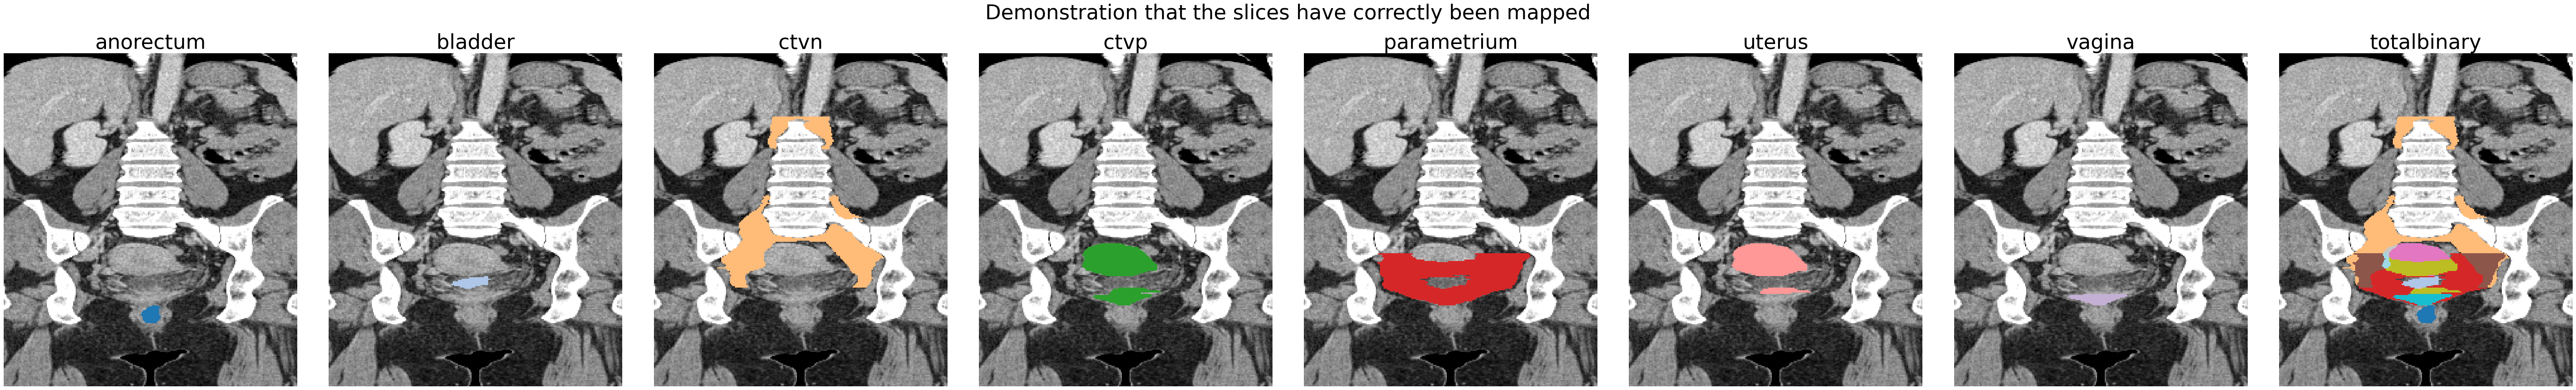
\includegraphics[width=.24\linewidth, trim=0 0 4400px 110px, clip]{../figures/check_if_worked_axis_1.png}}
  \subfigure[Bladder]{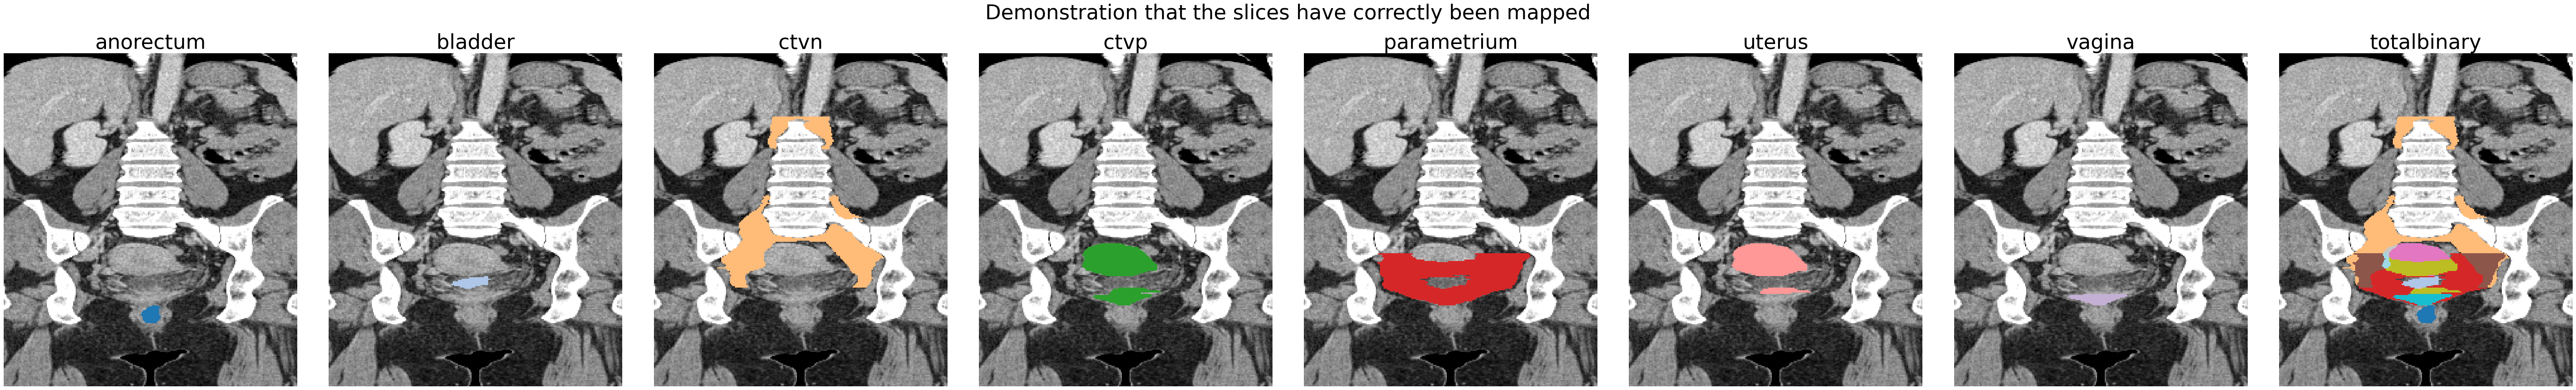
\includegraphics[width=.24\linewidth, trim=630px 0 3770px 110px, clip]{../figures/check_if_worked_axis_1.png}}
  \subfigure[CTVn]{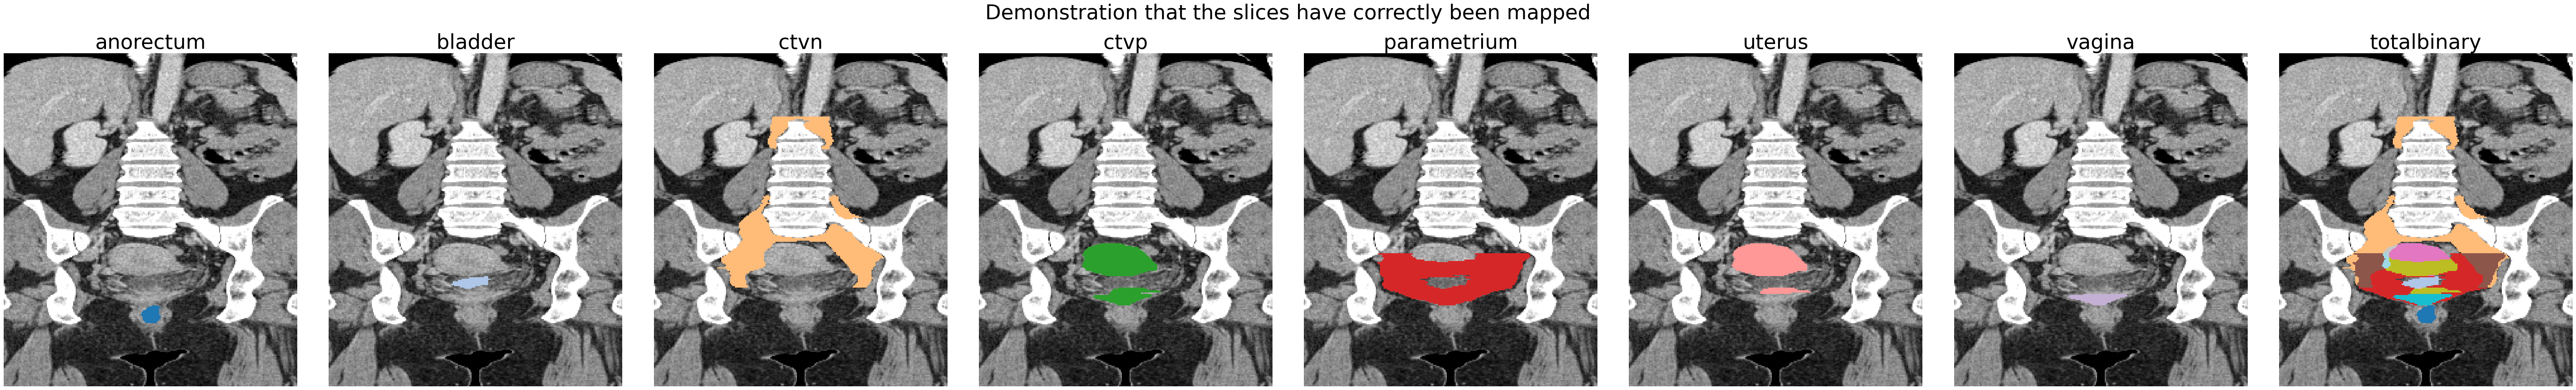
\includegraphics[width=.24\linewidth, trim=1260px 0 3140px 110px, clip]{../figures/check_if_worked_axis_1.png}}
  \subfigure[CTVp]{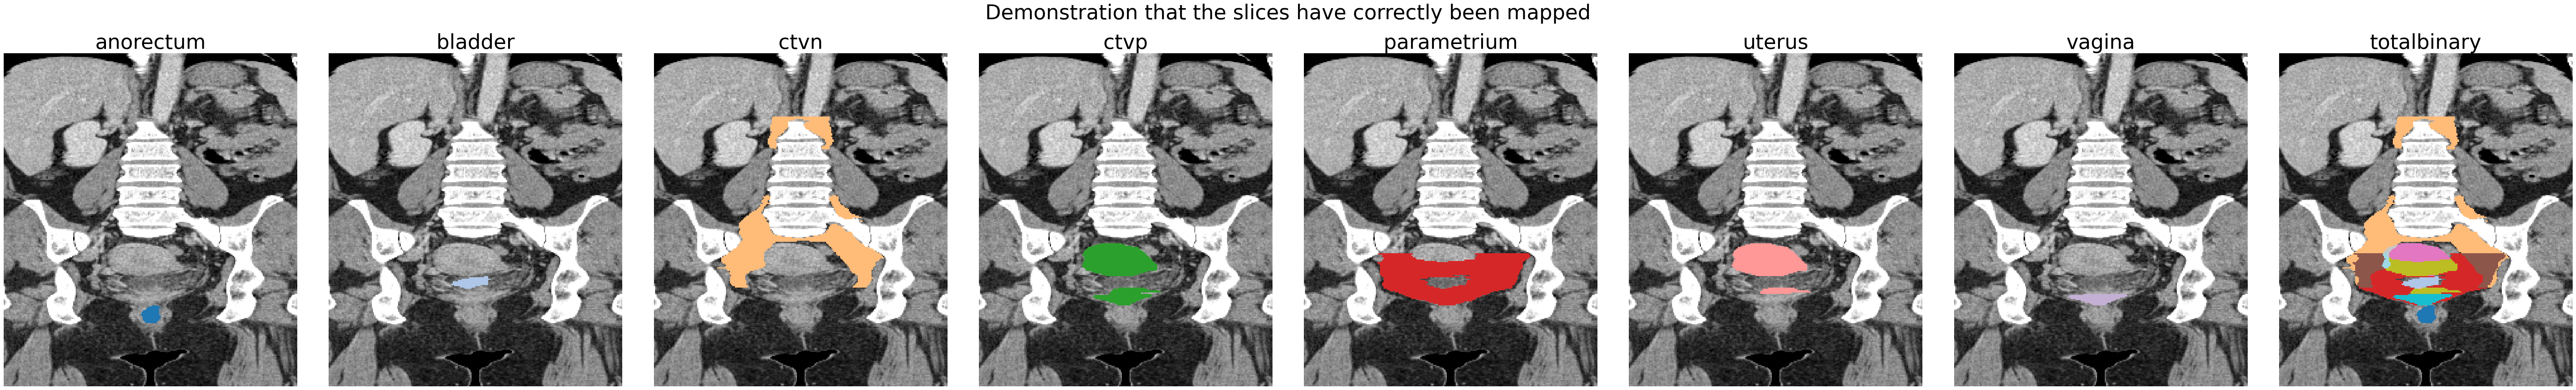
\includegraphics[width=.24\linewidth, trim=1890px 0 2510px 110px, clip]{../figures/check_if_worked_axis_1.png}}
  \subfigure[Parametrium]{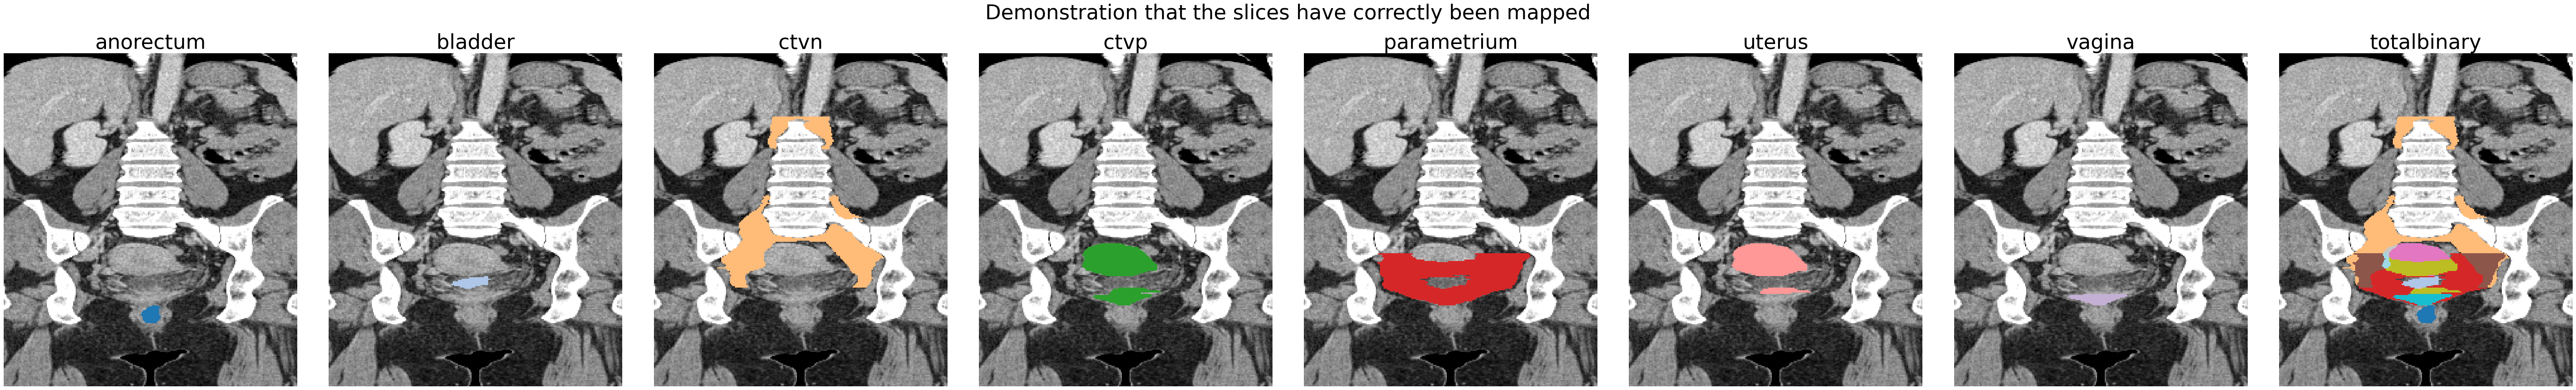
\includegraphics[width=.24\linewidth, trim=2520px 0 1880px 110px, clip]{../figures/check_if_worked_axis_1.png}}
  \subfigure[Uterus]{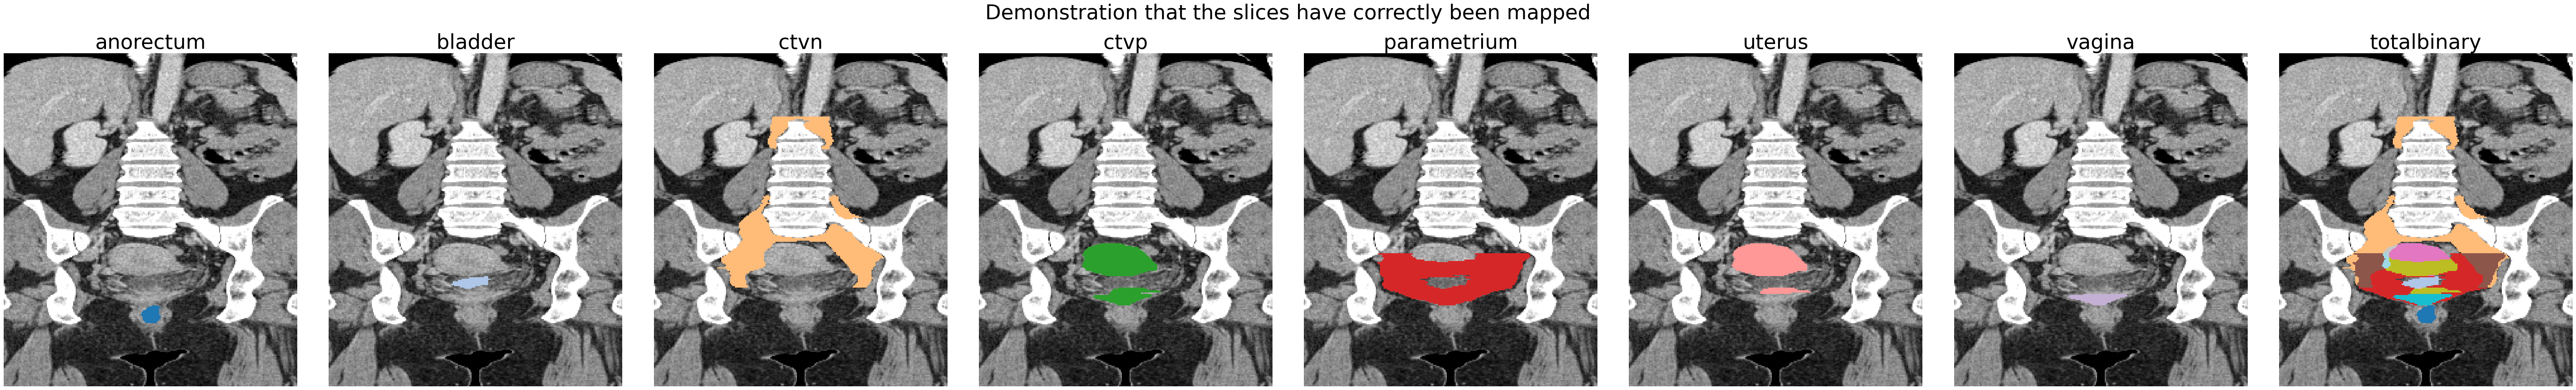
\includegraphics[width=.24\linewidth, trim=3150px 0 1250px 110px, clip]{../figures/check_if_worked_axis_1.png}}
  \subfigure[Vagina]{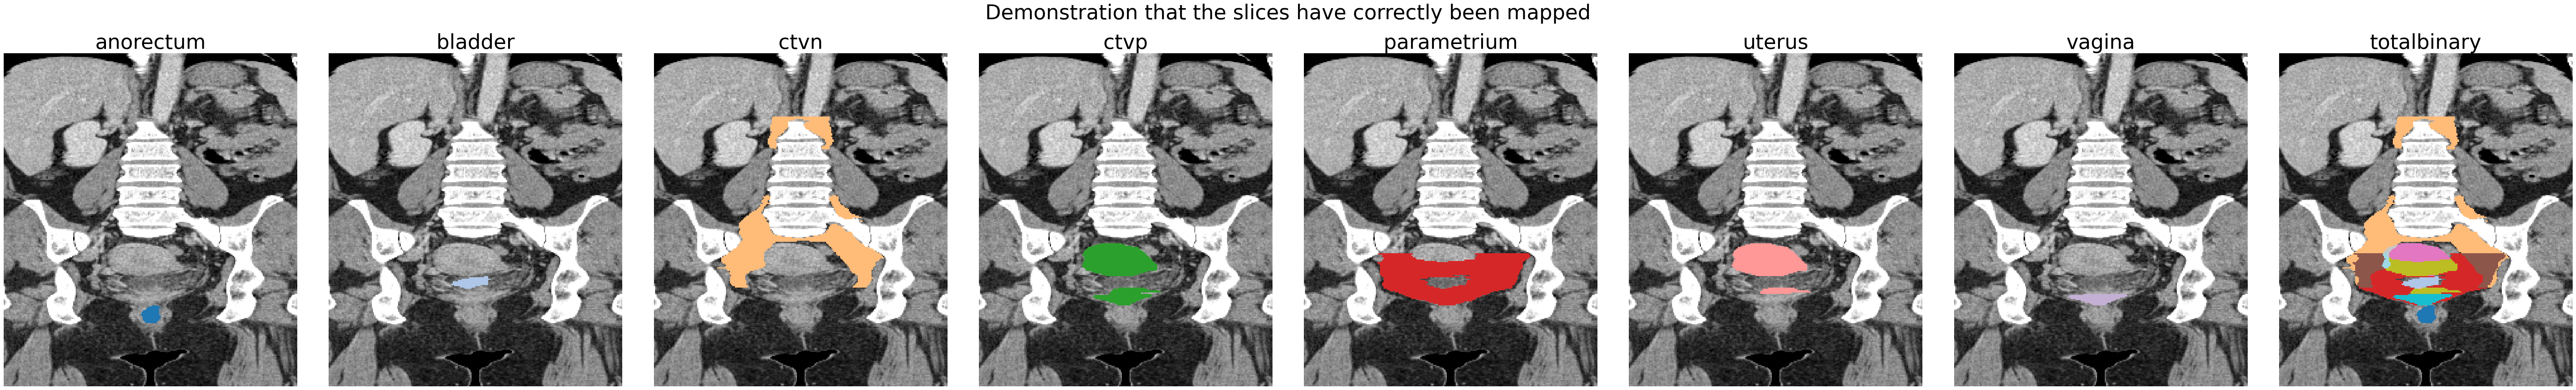
\includegraphics[width=.24\linewidth, trim=3780px 0 620px 110px, clip]{../figures/check_if_worked_axis_1.png}}
  \subfigure[Combined Labels]{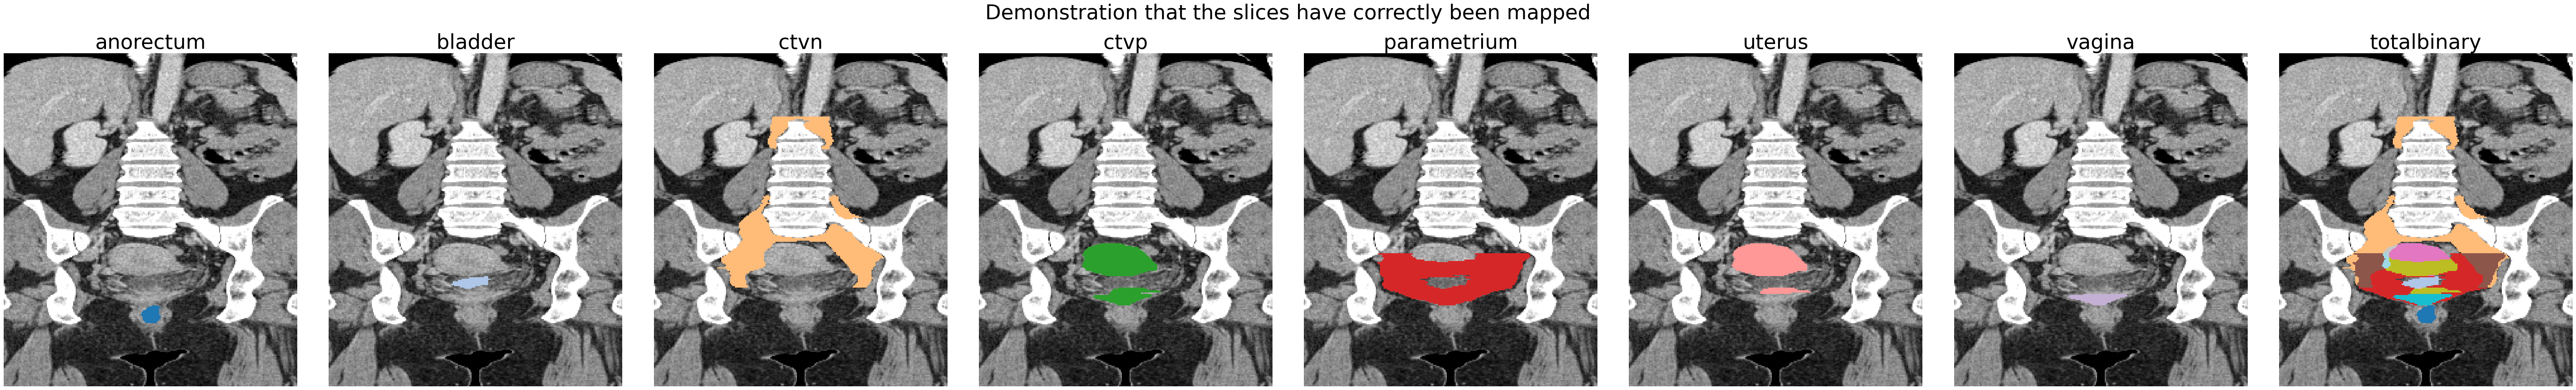
\includegraphics[width=.24\linewidth, trim=4430px 0 0px 140px, clip]{../figures/check_if_worked_axis_1.png}\label{fig:combined-labels-region-based}}
  
  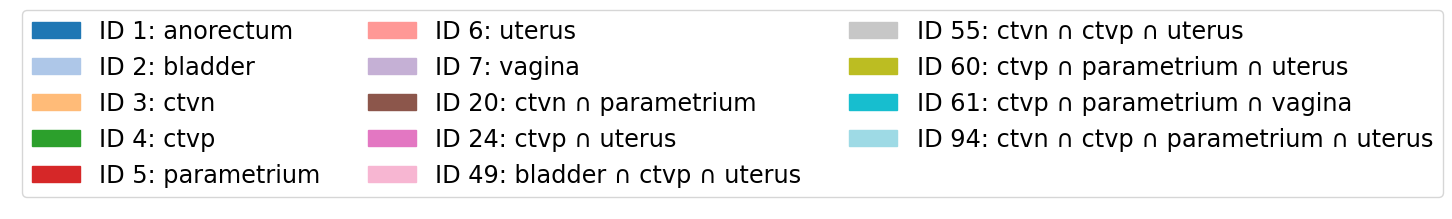
\includegraphics[width=\linewidth]{../figures/check_if_worked_axis_1_legend.png}
  
  \caption{New IDs generated for a single slice as a consequence of practical experience show non-conformity to rules in Section~\ref{sec:rules}.}\label{fig:check-if-worked-axis-1}
\end{figure}

The natural extension of separate training is to consider training each class simultaneously. Region-based training is a noninvasive method offered by the nnUNet. This training style combines the 3D segmentation maps for each of the seven classes into one 3D segmentation by introducing new IDs wherever there is a new overlap. An example slice can be seen in Figure~\ref{fig:check-if-worked-axis-1}.

\subsubsection{No Rule Enforcement}

Firstly, samples are preprocessed into a region-based format specified by the nnUNet pipeline; a new id is introduced for each new overlap. The model trains similarly on seven classes, with the objective of learning the segmentation patterns for each class. For comparison, an nnUNet network is trained in parallel to the fine-tuning of a TotalSegmentator model to evaluate the performance of the region-based training with transfer.

\subsubsection{With Rule Enforcement}

A sensible and calibrated set of ids could be drawn based on the rules in Section~\ref{sec:rules}. However, practical experience and the recalcitrant and challenging nature of defining logical expressions to generalize something as complex as organs and something as fuzzy as microscopic cancer spread mean that, in practice, these rules cannot be implemented strictly.

When considering the total sample set, the overlap makes up a minimal percentage of the total volume with non-background label classification. Figure~\ref{fig:illegal_overlap} shows all cases of `illegal' overlap found within the samples. The most frequent culprit overlap that breaks the condition is between the CTVn, CTVp and the Uterus. The Uterus is a necessary subset of the CTVp, which implies that this segmentation of CTVp does not include microscopic spread, including in the Cervix and GTVp. By eliminating this style of error from the model, it might be possible to obtain more general segmentations that align with the clinical team's rules.

% TODO: say that region-based learning without rule enforcement scored the same w.r.t illegal overlap because the model deosn't overfit on training data.

\begin{figure}[H]
  \centering
  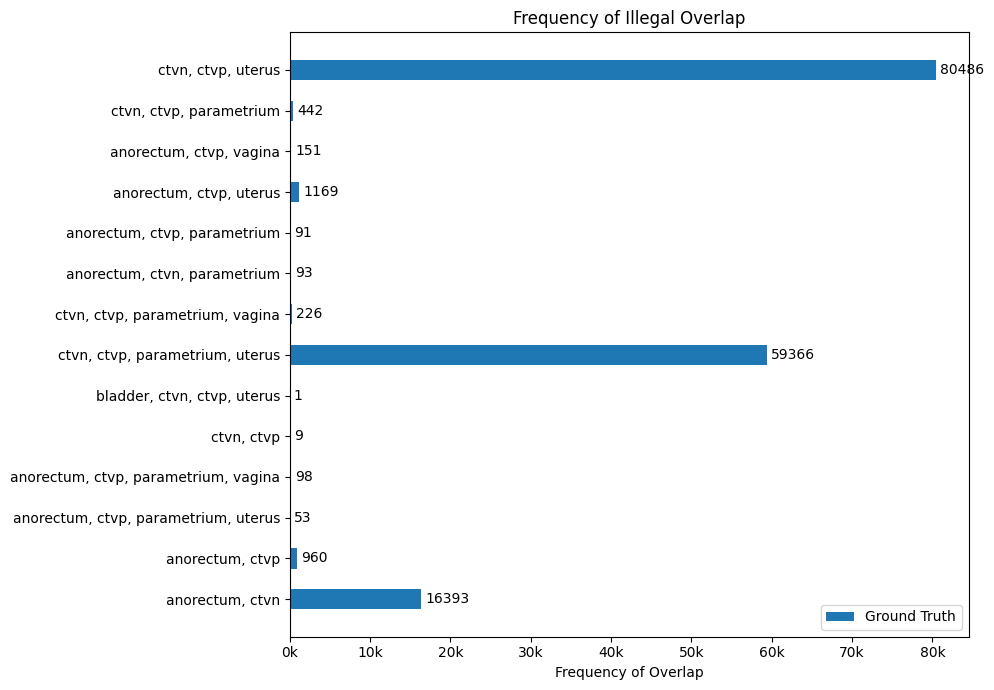
\includegraphics[height=.4\textheight]{../../research/source/code/nnUNet/3_gt_engineering/illegal_overlap_ground_truth.png}
  \caption{Total frequency and percentage overlap of non-zero occurrences of `illegal' overlap between the CTVn, CTVp, and Anorectum (Equation~\ref{eq:ctvn-ctvp-anorectum}).}\label{fig:illegal_overlap}
\end{figure}

We implement the rules with the hypothesis of generalisation despite the rules not strictly followed in practice. Therefore, an augmentation of the nnUNet trainer is necessary to capture this result. Specifically, we introduce an additional loss component dubbed `custom\_loss' during training. This custom loss parameter implements two of the many rules that the Royal Marsden Hospital clinical staff provided. The two rules are thoroughly discussed in Section~\ref{sec:rules} and are Equation~\ref{eq:ctvn-ctvp-anorectum} and Equation~\ref{eq:ctvp2}. 

To consistently include the loss parameter, we have two sub-loss objectives operating on dice loss (Section~\ref{sect:spatial-overlap-based}). The first captures Equation~\ref{eq:ctvn-ctvp-anorectum}, which focuses on the strict requirement that the CTVn, the CTVp, and the anorectum do not overlap. The loss term is minimal when the dice score is the lowest, indicating minimal overlap; thus, to calculate this result on the intersection, the implementation of vanilla dice loss applies to the rule's three permutations independently. Secondly, Equation~\ref{eq:ctvp2} insights more overlap between the vagina and uterus with the CTVp, which is equivalent to 1 minus the previous learning objective. As a hyperparameter, we attribute a weight of 0.3 to this term, while other loss terms (dice and binary cross-entropy) are assigned weights of 1 to keep the original objective function reasonably unchanged.

We hypothesise that although the rule-free model attempts to approximate the ground truth, which may call for marginal overlap, with the rules in place, this may generalise better over other cases.

\section{UniverSeg}

% \begin{figure}[H]
%   \centering
%   % 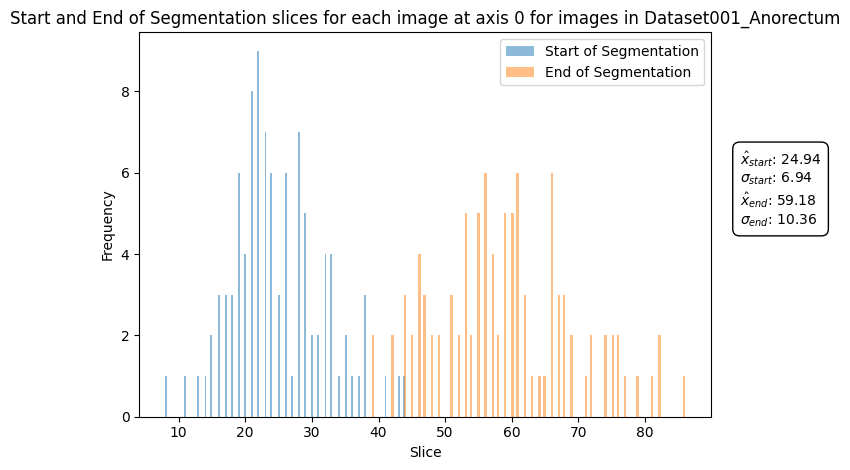
\includegraphics[width=.8\linewidth]{../../research/source/code/UniverSeg/start_end_distribution_axis_0_anorectum.png}
%   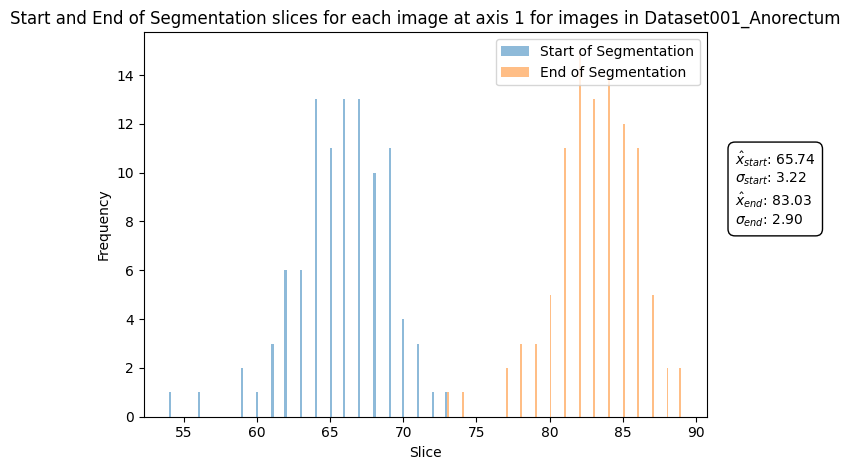
\includegraphics[width=.8\linewidth]{../../research/source/code/UniverSeg/start_end_distribution_axis_1_anorectum.png}
%   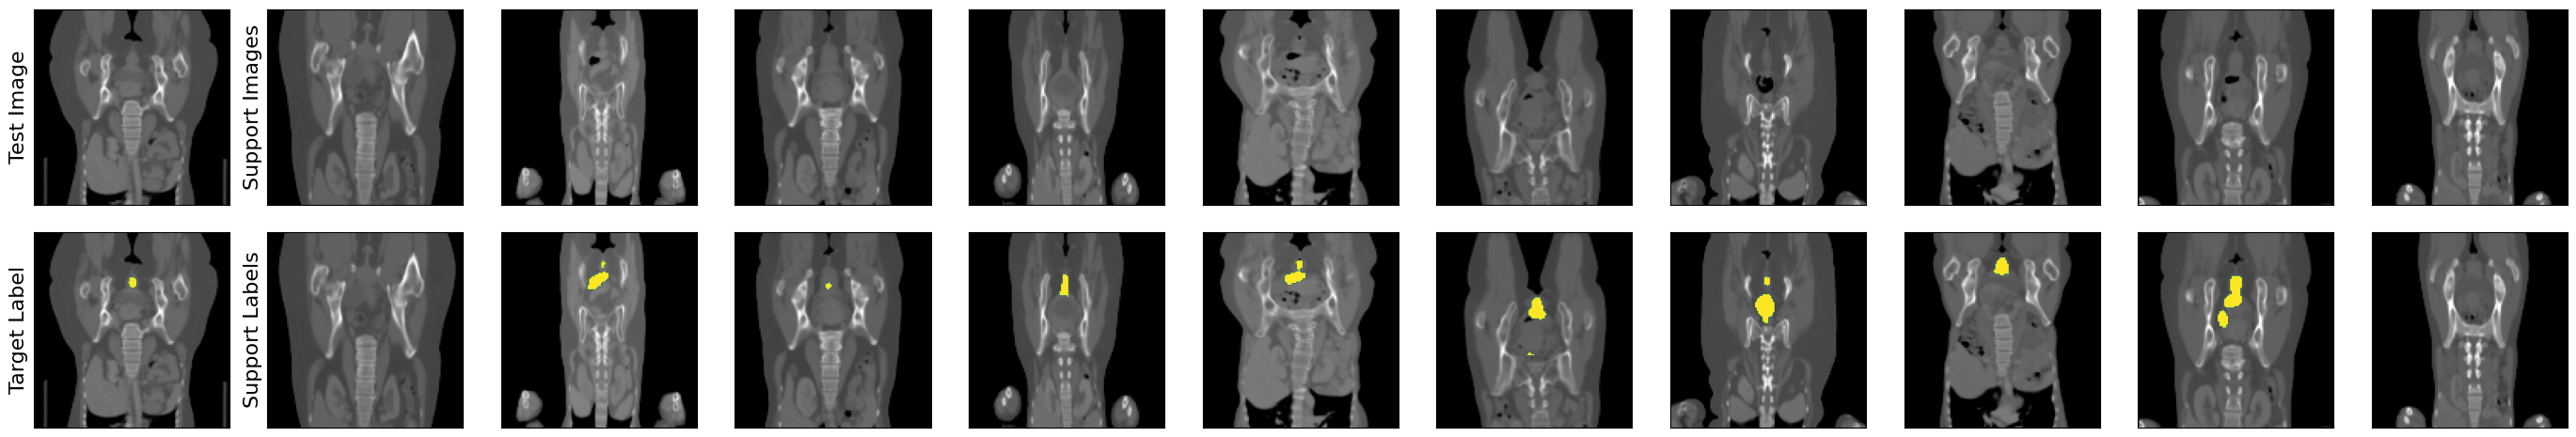
\includegraphics[width=\linewidth, trim=0 0 340px 0, clip]{../../research/source/code/UniverSeg/support_anorectum_axis_1.png}
%   % \subfigure[]{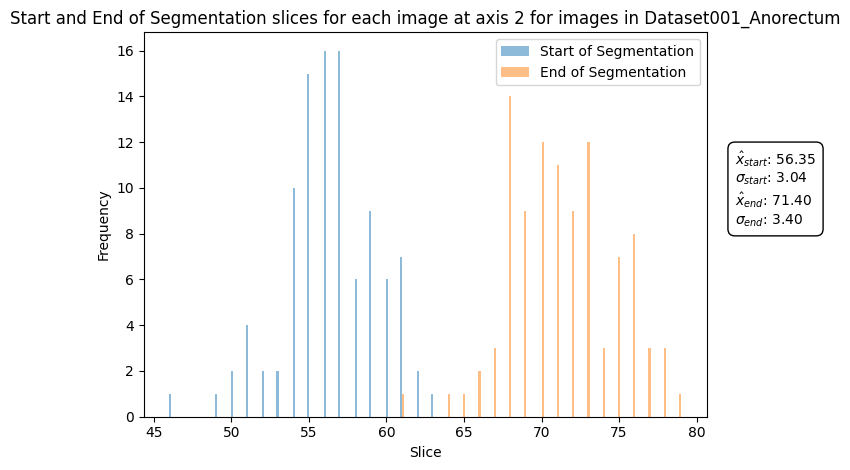
\includegraphics[width=.45\linewidth]{../../research/source/code/UniverSeg/start_end_distribution_axis_2_anorectum.png}}
%   \caption{The distribution of the start and ending slices of the tumor in a normalized batch of images across axes 1 (sagittal dimension) and the corresponding sampled support extracted.}\label{fig:start-end-distribution-universeg}
% \end{figure}

UniverSeg operates on 2-dimensional data. As a result, to provide automatic radiotherapy planning volumes, it is essential to provide slices for the model as input alongside a sufficient support size of similar slices. This network allows discussions for few-shot transfer into the radiotherapy domain.

\subsection{Preprocessing}

Images are normalised to match UniverSeg's training properties. Specifically, image intensities are clipped to the range $[-500, 1000]$ and normalised to be between $[0,1]$ and finally scaled down to a $128 \times 128$ resolution~\cite{universeg}. Slice pre-processing is repeated along each axis to evaluate the effectiveness of one slice over another. 

% \subsection{Automated Support Set Sampling}

% The most screaming disadvantage of such a model when applied to a three-dimensional unseen segmentation task is tumour localisation; we do not know where the tumour starts or ends. The tumour's location can only be determined by referring to assisting models that provide estimates or make assumptions about tumour location based on previous examples. In a secluded environment where only one's model transferability is assessed, we instead analyse the properties of the tumour from the examples.

% We begin by analysing the tumour locations along each axis. The intuition is that the pre-processed images of equal dimensions and spacings should contain the tumour at approximately the same location. Figure~\ref{fig:start-end-distribution-universeg} shows the tumour's distribution of start and end slices and the corresponding sampled support set.

% By sampling a support set concerning slice positions, we include an approximation of a binary classification of `does this slice contain a tumour or not'; if for slice $n$ there is a 20\% chance that the support contains a tumour, then we can also assume that for an unseen patient, this chance is also the same. However, this does not generalise to boundary cases where tumours or organs may begin sooner or later than all others, which may cause a misclassification.

\subsection{Supervised Support Set Sampling}

To consider this model's overall transfer ability, we also consider a supervised setting; the model is fine-tuned on each axis of every anatomy across a spectrum of tumour locations across a specific axis. The support set is sampled from the query on the same anatomy and along the same axis. As a result, seven fine-tuned models are trained for each anatomy and axis on which the contour is located.

Authors in UniverSeg tested performance on central slices along 3D volumes~\cite{universeg}. However, the model's performance on the central slice is not indicative of the model's performance on the entire volume. To investigate this further, we will continue with a heavily supervised setting. In this setting, support slices are generated from any patient's slices containing a contour, allowing us to more accurately assess the model's performance across the entire volume. 


% The main difference from the previous implementation is that we always expect a contour to be produced from the query, and we always know the support will have variable segmentations across the axis.

\section{MedSAM}

MedSAM is the final algorithm in the shot-learning strategies that will be covered. Specifically, MedSAM is being evaluated on the provided dataset, both with and without transfer, to test the claim of transferability.

Zero-shot learning, a promising feature of MedSAM, could potentially enable it to handle tasks it has never encountered before. However, the assertion that it can seamlessly transfer without refinements is a bit of a stretch. This is because certain contours, like the CTVn, delineate tiny tumor spread throughout the lymph node system. Therefore, it is unlikely that MedSAM, trained in such cases, would be used for these specific tasks. It would typically be used for more straightforward volume delineations, such as organs.

\subsection{Preprocessing}

MedSAM takes two-dimensional images as input, much like UniverSeg. Therefore, we similarly preprocess the data to a resolution of $1024 \times 1024$ along each slice where the ground truth is present. We clip the ranges of the CT scan to Hounsfield units centred around the 40 value, with a window radius of 400 units and later normalized to the range of $[0,1]$. In contrast to UniverSeg, we resize a slice after selecting the index instead of resizing the whole image. Thus, we do not introduce any anisotropic uncertainties along our sampling axis.

Further, in contrast to previous strategies, the MedSAM preprocessing step also removes ground truth segmentations that occupy an area below a specified threshold. The idea here is that the challenge with locating the small areas of the region of interest is an entirely different classification of the problem; the issue is with object detection instead of object segmentation~\cite{SAM, Ma2024}. This detail of the preprocessing is critical to consider for discussion and use as this would increase the proposed surface distance along an axis.

% \subsection{Point based transfer}

% The default MedSAM architecture offers a point based prompt, and also a box based prompt. However, points are not a consideration for this 

% We first experimented with the MedSAM architecture to test the effectiveness of prompting on points. The baseline MedSAM implementation offers a point based prompt and also a box based prompt. To consider both mediums of prompt encoding, we can consider a sparse and desnse point planning. % We formulated this task into two categories: a sparse and dense point experiment.  

% \begin{figure}
%   \centering
%   \raisebox{-0.5\height}{\subfigure[Sparse point prompt]{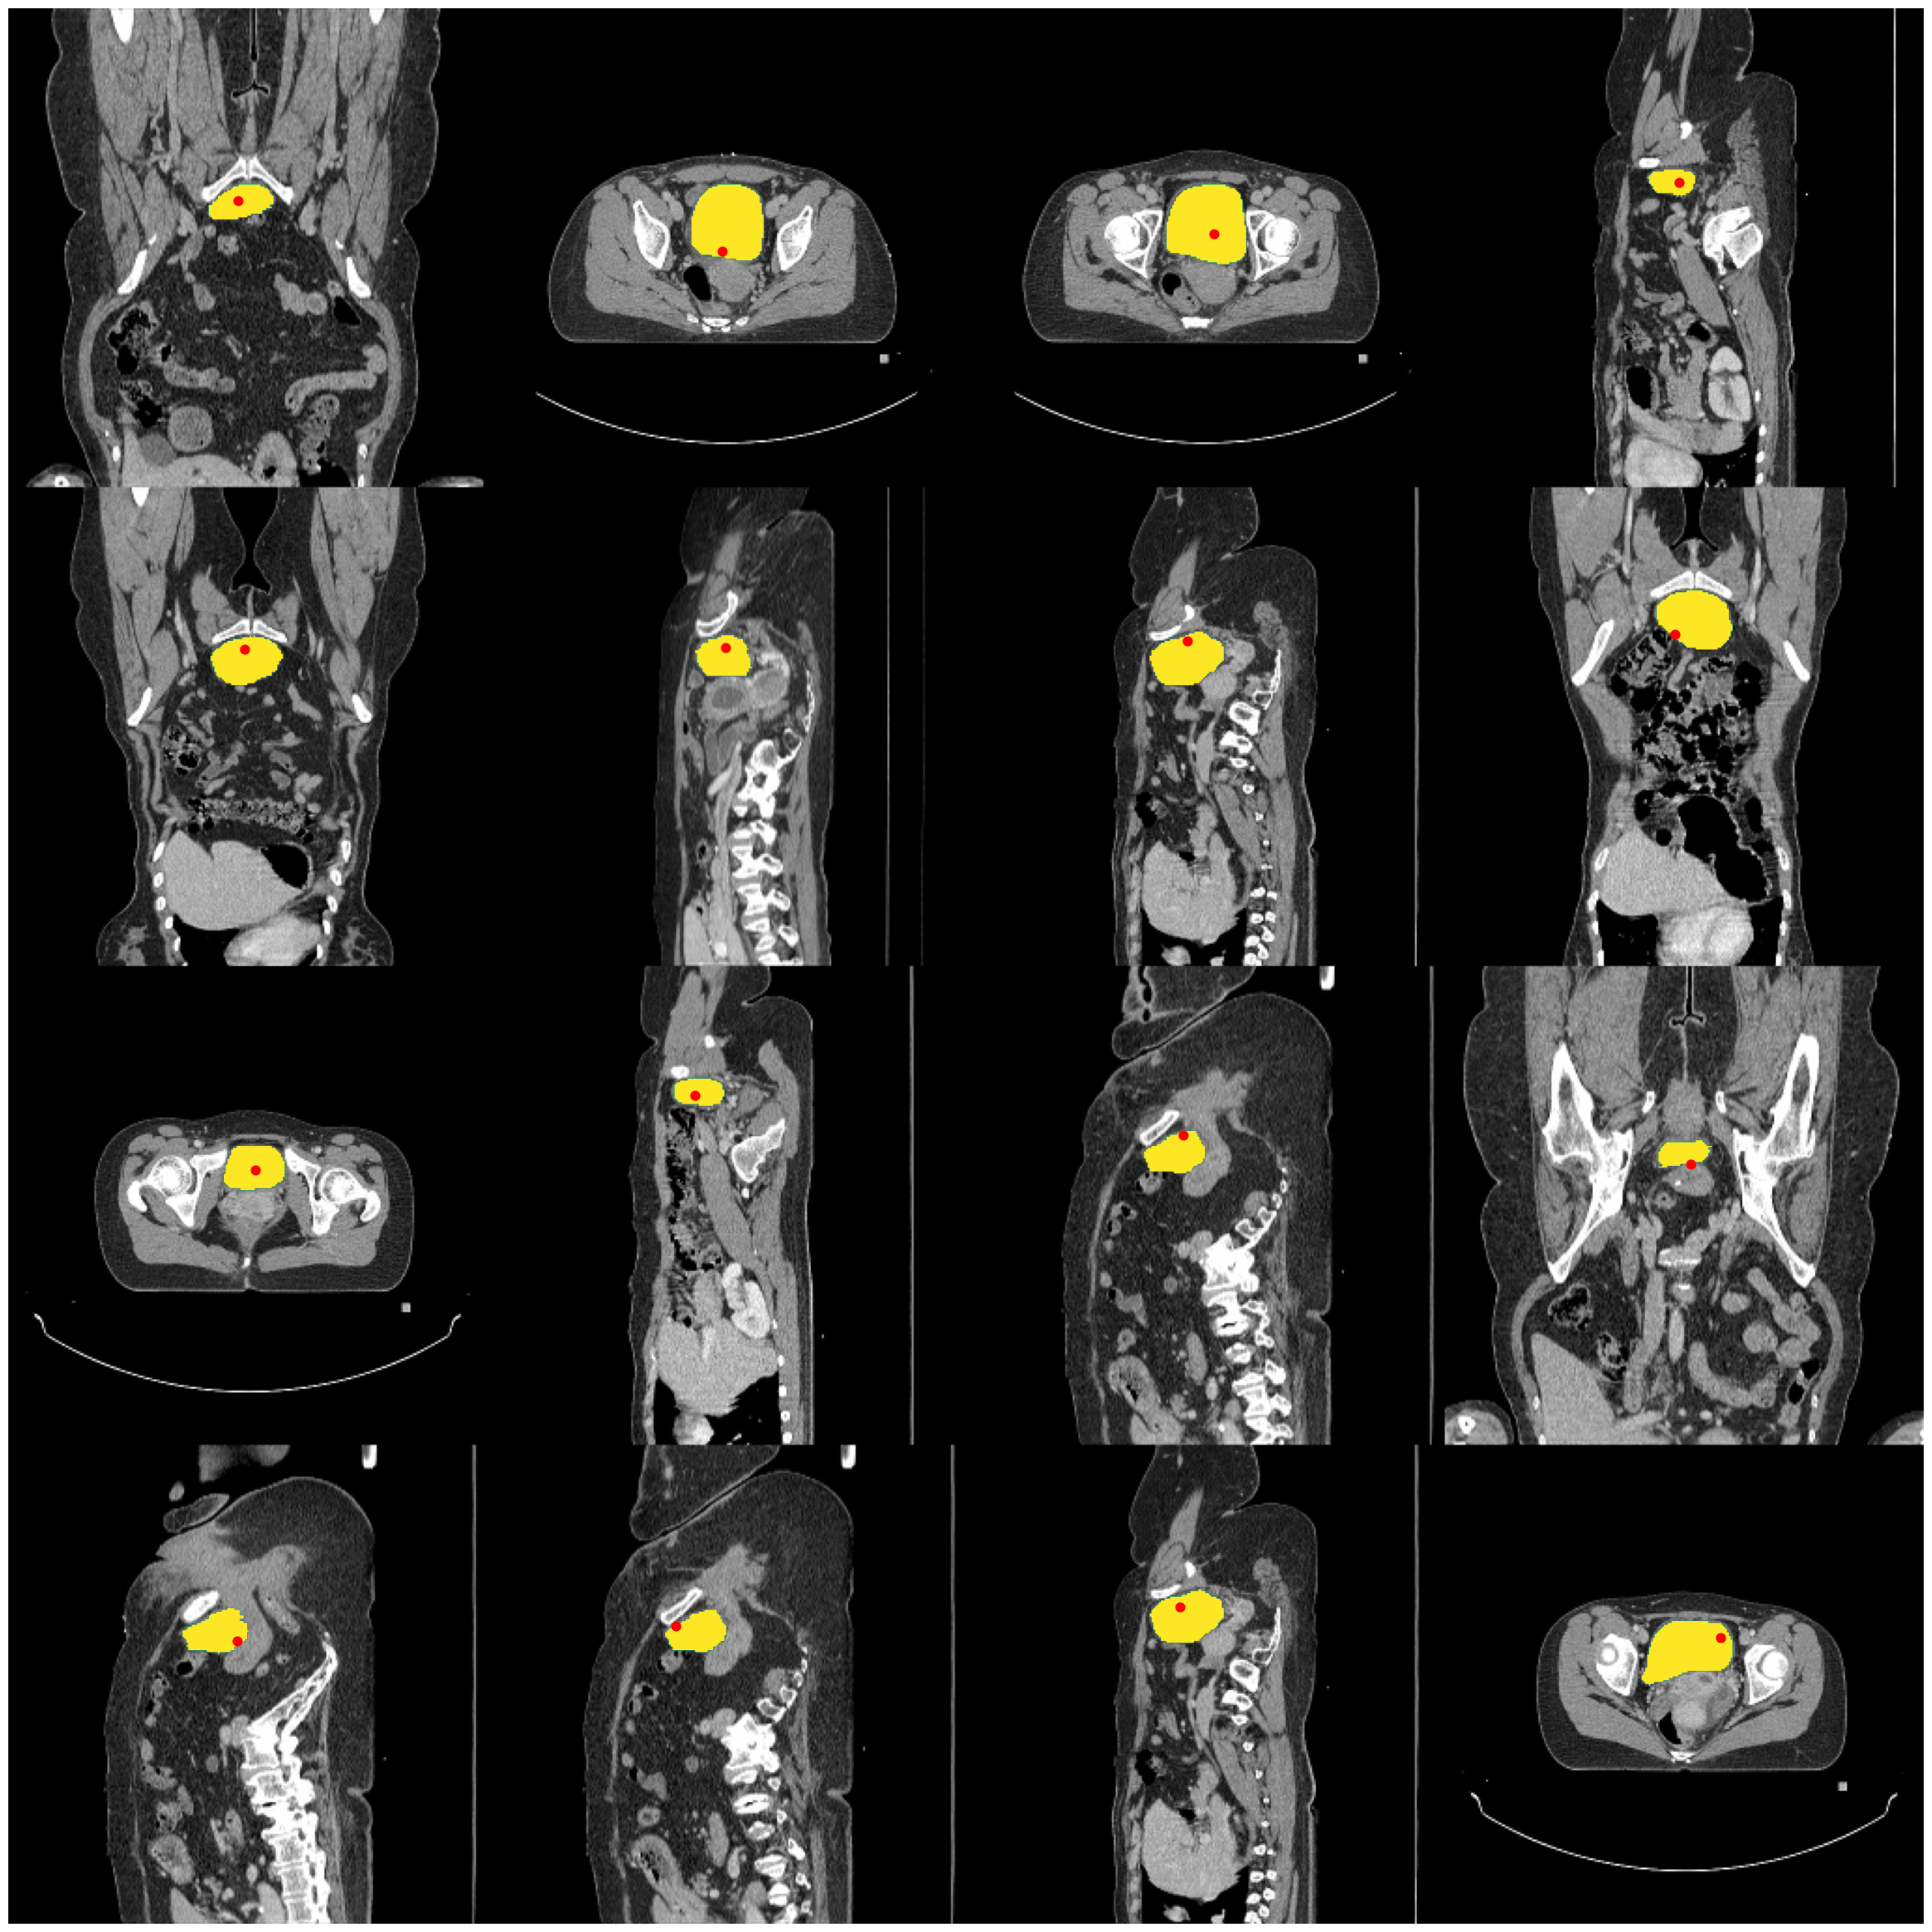
\includegraphics[width=.45\linewidth, trim=850 850 0 0, clip]{../../research/source/code/SAM_Med/3_train_point_prompt/point_batch_example.png}}}
%   \raisebox{-0.5\height}{\subfigure[Dense point prompt]{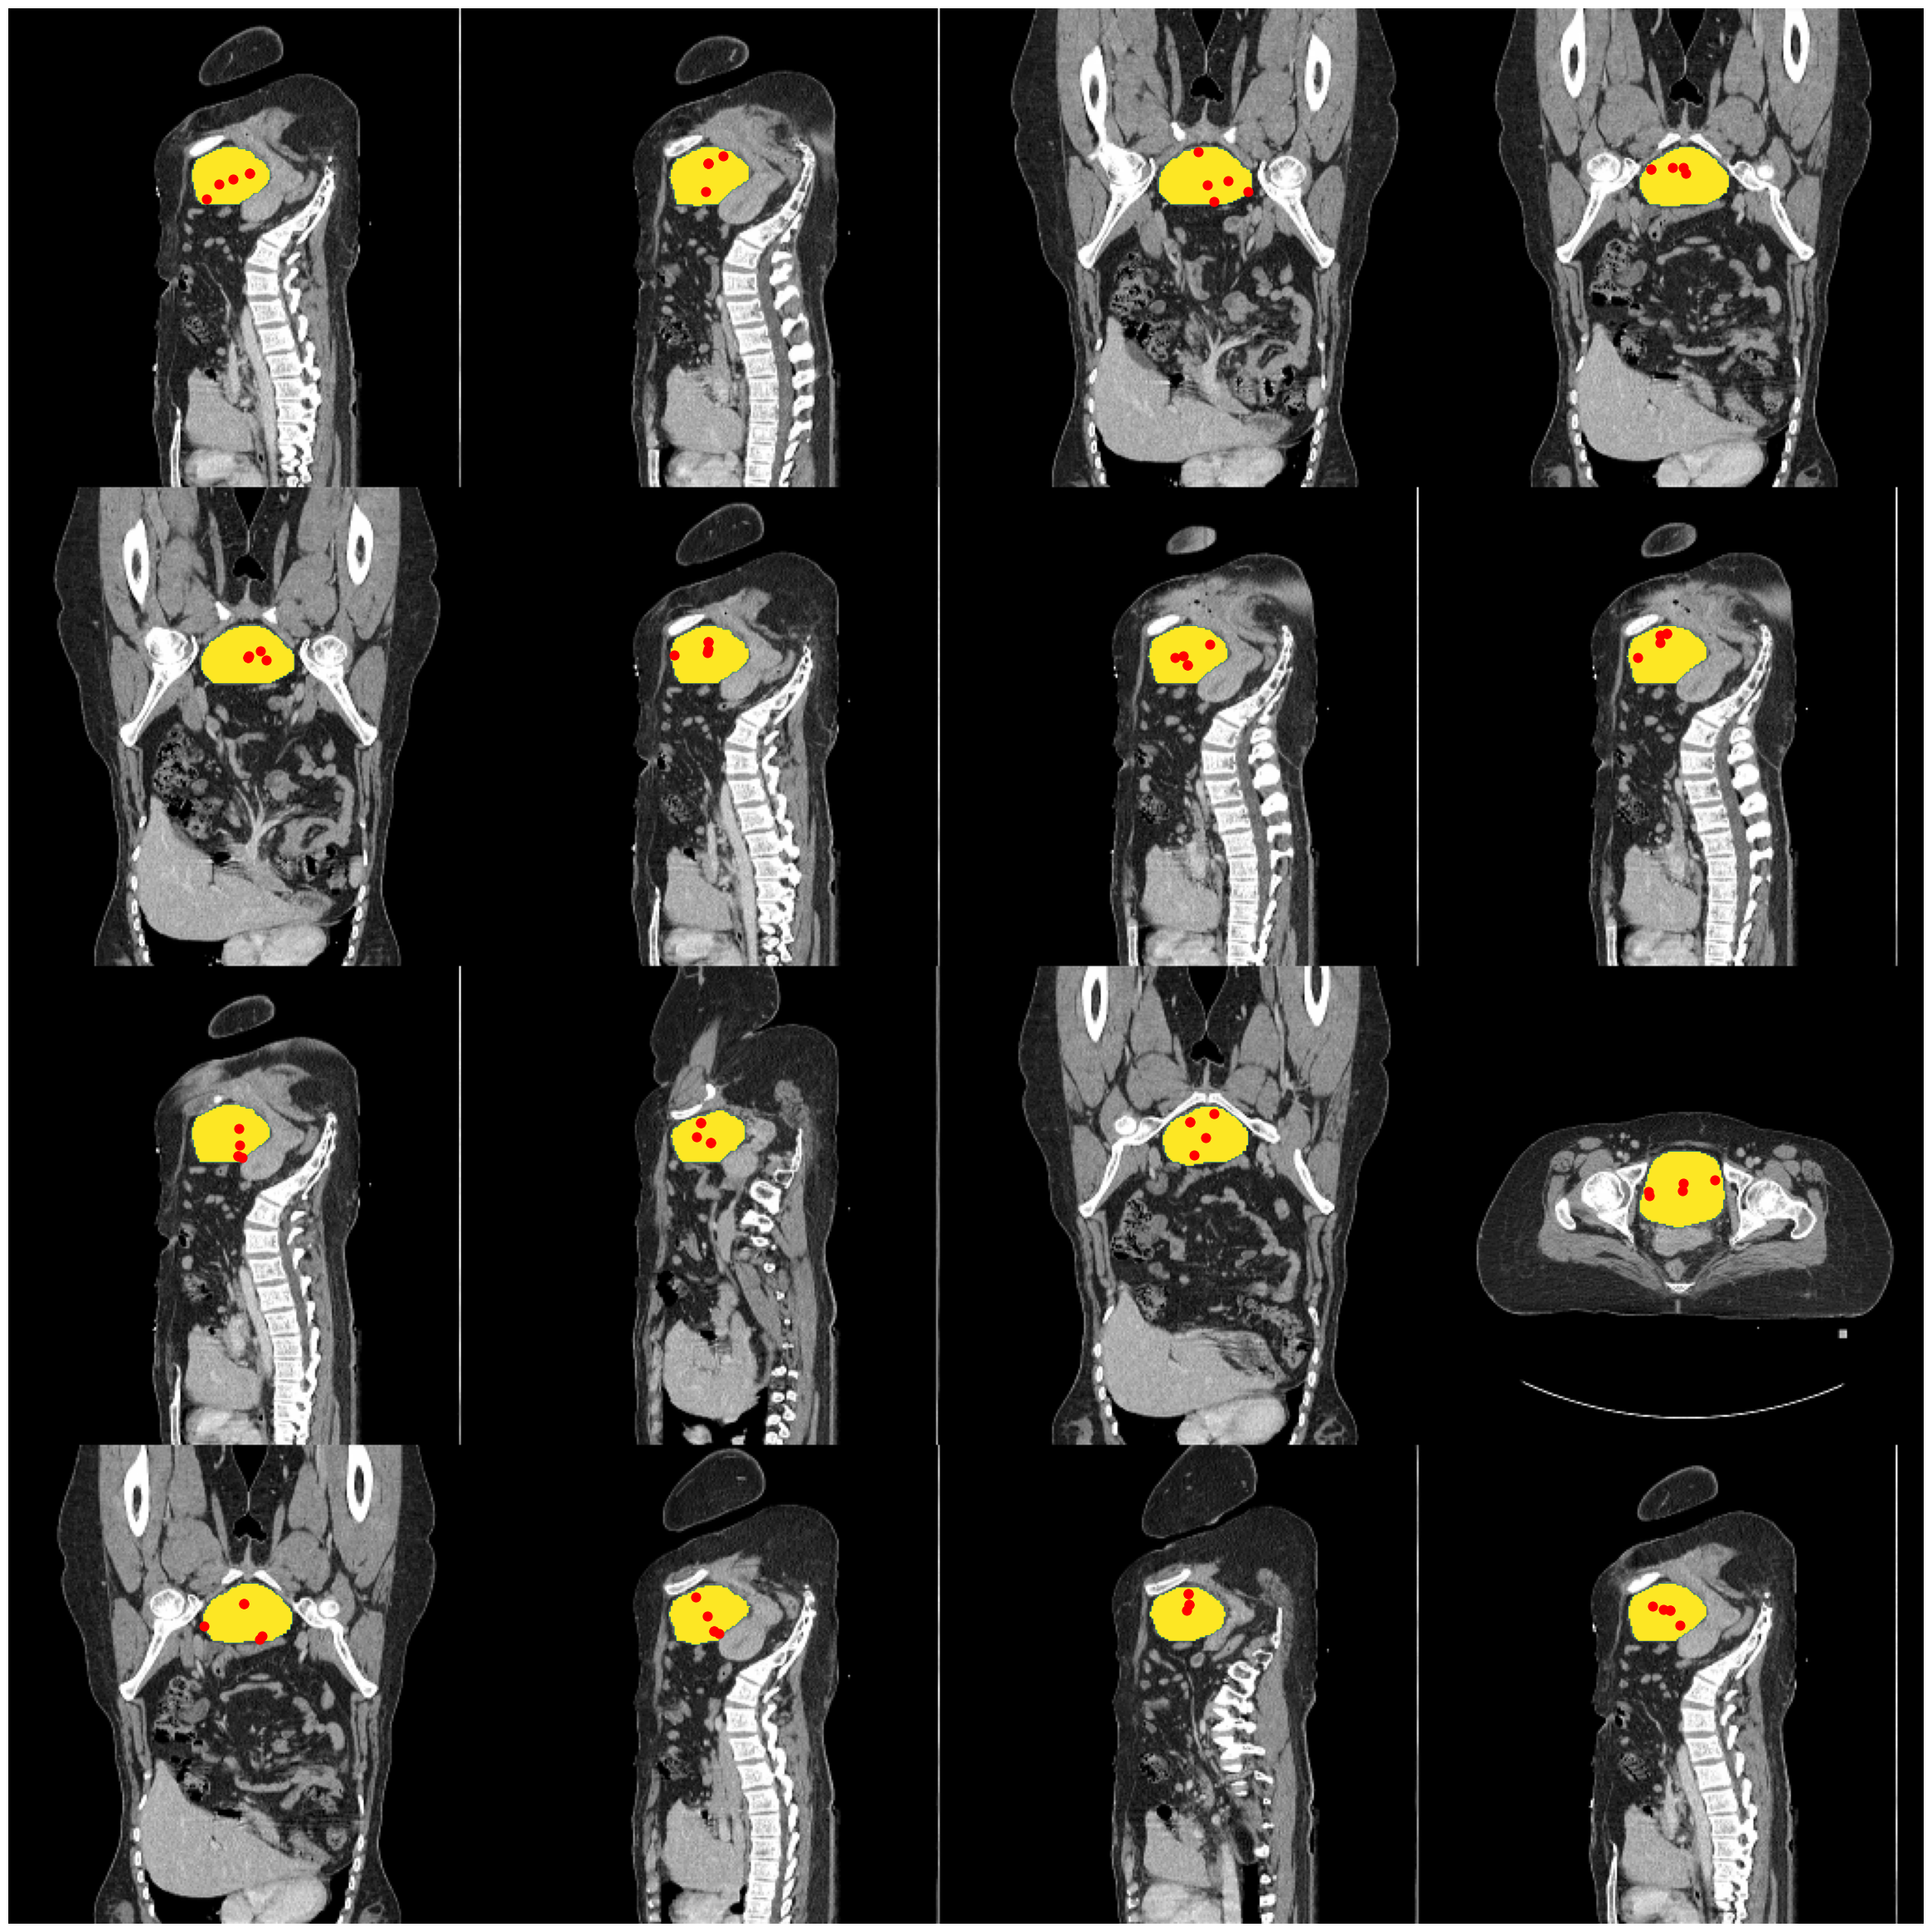
\includegraphics[width=.45\linewidth, trim=0 0 850 850, clip]{../../research/source/code/SAM_Med/3_train_point_prompt/point_dense_batch_example.png}}}
%   \caption{The two strategies for sampling structures in the MedSAM model.}\label{fig:point-prompt}
% \end{figure}

% The two strategies are shown in Figure~\ref{fig:point-prompt}. The sparse point prompt is a single point in the image, while the dense point prompt is a set of $n$ points randomly sampled from the ground truth segmentation.

% The hypothesis is that point prompts may work well with structures such as the bladder which are trivial to identify. However, for the CTV, the point prompt may not segment the full extent of the structure.

% Points are sampled with a higher probability of being towards the centre of the segmented area by calculating the Euclidean distances of all points from the centroid. This heuristic dispels any ambiguity that may be caused when selecting points closer towards the outline of the segmentation, which may occur when boundaries of different objects bleed into one another, causing a higher error.

% This strategy, however, is not enough; the MedSAM model often provides whispy boundaries in a response to the point prompts as it must work harder at guessing the boundaries of the object. Therefore, this strategy is dispelled from consideration.

\subsection{Box based transfer}

\begin{figure}
  \centering
  \subfigure[Boxed ground truth image]{
    {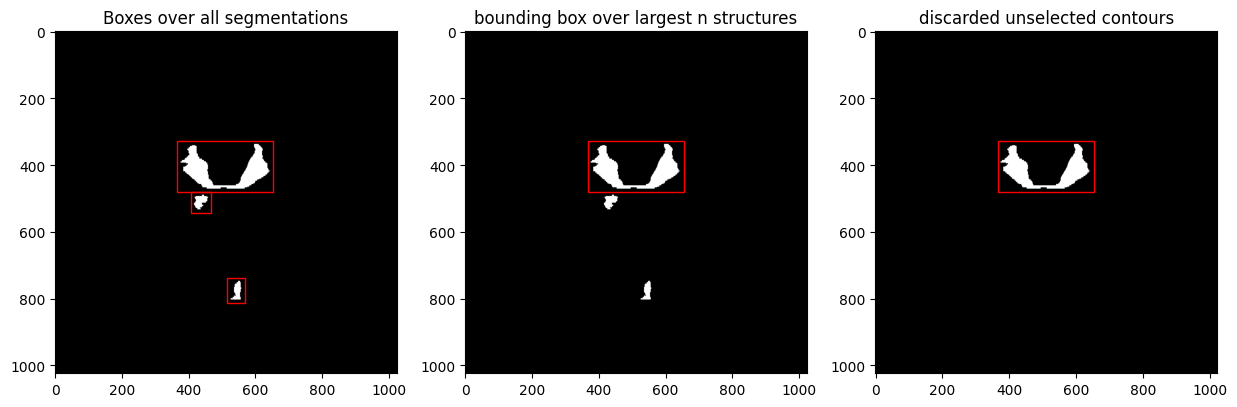
\includegraphics[width=.3\linewidth, trim=40 30 610 30, clip]{../../research/source/code/SAM_Med/4_train_box_prompt/select_top_n_largest_structures.png}}
  }
  \subfigure[Selected tumor boxed]{
    {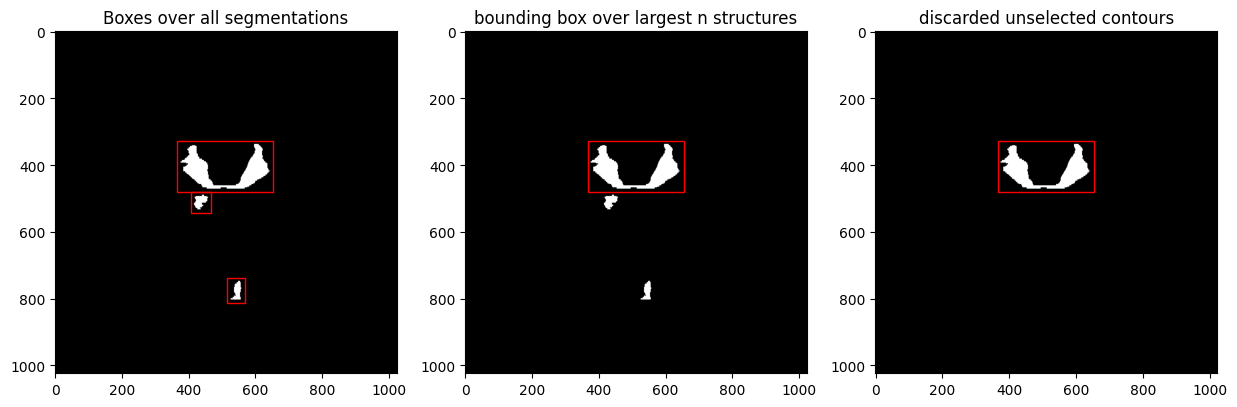
\includegraphics[width=.3\linewidth, trim=340 30 310 30, clip]{../../research/source/code/SAM_Med/4_train_box_prompt/select_top_n_largest_structures.png}}
  }
  \subfigure[Adjusted Ground truth]{
    {\includegraphics[width=.3\linewidth, trim=630 30 20 30, clip]{../../research/source/code/SAM_Med/4_train_box_prompt/select_top_n_largest_structures.png}}
  }
  \caption{The process of selection bounding box for a given boxed tumor with an augmented ground truth used at training time for the MedSAM bax-based prompt model.}\label{fig:box-prompt-sam-selection}
\end{figure}

A box prompted solution will define the area where the tumour is likely to be. Box prompts for training are obtained from the ground truth, with a margin surrounding the box\footnote{An alternative approach would be to include points into the position encoder. However, limited tests demonstrated that transfer did not succeed and left predictions as a whispy and innacurate segmentation.}.

For training, only one box may be fed into the model for inference. Therefore, we select a random structure from the boxes encompassing the tumour for a given slice. Figure~\ref{fig:box-prompt-sam-selection} demonstrates the tumour box selection at training time. 

Furthermore, images are augmented with a random rotation, scaling, and translation to improve generalisation. Data augmentation ensures that the model does not overfit the training data and can generalise to unseen examples.

% \subsection{Training Bottlenecks}

% \begin{figure}[H]
%   \centering
%   \subfigure[Raw epoch time before optimizations]{\includegraphics[width=.45\linewidth, trim=0 0 0 360px, clip]{../../data/MedSAM_finetuned/boxed_lowres/Anorectum/progress.png}}
%   \subfigure[Epoch time after pipeline optimizations]{\includegraphics[width=.45\linewidth, trim=0 0 0 360px, clip]{../../data/MedSAM_finetuned/boxed_lowres_2/Anorectum/progress.png}}
%   \caption{Comparison of epoch times for an expensive MedSAM model before and after pipeline optimizations.}\label{fig:training-comparison-med}
% \end{figure}

% This model requires three channels of $1024 \times 1024$ image slices, making each input image in its raw state a costly sample to send over the network especially after considering that each channel is a duplicate to match the requirements of the SAM model. This makes training on commodity hardware a difficult thing to accomplish. Training times can be very long without adding changes to the training pipeline. Figure~\ref{fig:training-comparison-med} compares training pipelines and performance improvements. 

% Firstly, image slices are stored in a $(1 \times 512 \times 512)$ resolution and upsampled before the forward pass. Furthermore, caching~\cite{charlie-caching} stored these smaller images on the training node to avoid repeated and expensive reads over the network. This improved training epoch times by 50 times.

\subsection{Evaluation}

During training, the test set is divided by ID to ensure that a portion of an image is not both trained and validated. This way, the model's transferability is not questioned because it is trained on a disjoint set of patients; otherwise, quantitative measurements would skew and not represent the model's adaptability to unseen data.

% Secondly, the MedSAM architecture selects points and boxes for inference from the ground truth. Because MedSAM is an interactive tool, its application will likely adapt as an assisting tool for clinicians. However, for unseen examples, the concept of auto planning is uncertain.

The authors of the paper measure performance according to the ground truth~\cite{SAM, Ma2024}. Refining the model pipeline to include bounding box predictions extracted from a baseline like nnUNet is possible, where MedSAM acts as a refinement to an already reasonably accurate guess. This allows for noise to be permeated into the model, thus allowing for a better auto-contour planning pipeline. However, we provide boxes from the ground truth because the MedSAM model is most well suited for interactive use. therefore, it is something that clinicians can use to cast a prediction, and refine it as necessary.

\section{Quantiative Evaluation of Segmentation}\label{sect:performance-evaluation}

Calculating the difference between the provided labelled data would be one way to determine if a contour can be used in a clinical context. However, we have different ways to evaluate this measure in a delineation context.

If we were attempting to fit a model onto a line in 2D space, the performance of our model would be the total minimum distance between each point and the prediction. Our objective would be to drive the model's distance metric as close to 0 without overfitting. Here, the points act as a 'ground truth', alternatively referred to as the gold standard, which represents the actual measured value.

The reasoning above extends to 3D and 2D in a segmentation context with variants to measure other quantities, like the minimum distance between prediction and truth or the extent of volume overlap between the two. These are examples of geometric measures, which Mackay et al. has found to be the most popular measure in segmentation tasks~\cite{review-metrics}.

\subsection{Classification Based}\label{sect:classification-based}

Assesses if voxels within and outside the auto-contour have been correctly labelled~\cite{review-metrics}. To begin, we define 'positive' to mean that the voxel selected indeed needs radiotherapy treatment and 'negative' to mean that the voxel classifies as healthy.

A standard measure of classification is accuracy. It measures the total number of correct predictions vs. the total predictions it made. However, more than this measure is needed to fully capture a model's bias because it does not tell the whole story with class-imbalanced data when there is no even number between positive and negative labels.

\begin{equation*}
 \text{Accuracy} = \frac{TP + TN}{TP + TN + FP + FN}
\end{equation*}

Better measures are Precision and Recall scores. The Precision (also known as the Positive Predictive Value~\cite{evaluation-metrics}) measures the proportion of successfully correct predictions. The Recall (also known as True Positive Rate~\cite{evaluation-metrics}), on the other hand, ``measures the portion of positive voxels in the ground truth that is also identified as positive by the segmentation being evaluated''.

\begin{equation*}
 \text{Precision} = \frac{TP}{TP+FP}, \quad \text{Recall} = \frac{TP}{TP+FN}
\end{equation*}

\subsection{Spatial Overlap Based}\label{sect:spatial-overlap-based}

Similarly to classification-based metrics in Section~\ref{sect:classification-based}, an overlap-based metric measures the extent of overlap between an auto-contour and a reference structure~\cite{review-metrics}.

The scores above combined into a more general score $F_\beta$ to give

\begin{equation*}
 \text{F}_\beta = (1+\beta^2)\cdot \frac{\text{Precision} \cdot \text{Recall}}{\beta^2 \cdot \text{Precision}+\text{Recall}}
\end{equation*}

A specific case of this equation with $\beta=1$ is mathematically equivalent to the DICE Similarity Coefficient. A review found that DICE is the most popular evaluation metric amongst 2021 studies~\cite{review-metrics,evaluation-metrics, Sherer2021-le}.

% \begin{align*}
%   F_1 = \text{DICE} & = \frac{2 \cdot \text{Precision} \cdot \text{Recall}} {\text{Precision} + \text{Recall}} & \\ 
%   % & = \frac{2 \cdot \frac{TP}{TP + FP} \cdot \frac{TP}{TP + FN}}{\frac{TP}{TP + FP} + \frac{TP}{TP + FN}} \\
%   % & = \frac{2 \cdot TP \cdot TP}{TP(TP+FN)+TP(TP+FP)} \\ 
%   & = \frac{2 \cdot TP}{2TP + FP + FN} \quad = \quad \frac{2|S_g^1\cap S_p^1|}{|S_g^1|+|S_p^1|} , \text{where} \begin{cases}
%     S_g^1 & \text{ground truth} \\
%     S_p^1 & \text{segmentation}
%   \end{cases}
% \end{align*}

\begin{equation*}
 F_1 = \text{DICE} = \frac{2 \cdot \text{Precision} \cdot \text{Recall}} {\text{Precision} + \text{Recall}} = \frac{2 \cdot TP}{2TP + FP + FN} \quad = \quad \frac{2|S_g\cap S_p|}{|S_g|+|S_p|}
\end{equation*}

Where $S_g$ is the ground truth segmentation and $S_p$ is the predicted segmentation. From this relationship, the DICE score has found popularity in image segmentation for similar reasons that the $F_1$ score has found its popularity in classical machine learning; it can provide a fair result for imbalanced datasets. This mentality is applicable in our scenario because a tumour will make up very little of the total volume of the domain space. This argument extends to a Volumetric DSC by considering the above in all three dimensions~\cite{APL}.

Another popular related evaluation method is the Jaccard Index, which measures the intersection over the union of two sets:

\begin{equation*}
 \text{JAC} = \frac{TP}{TP+FP+FN} = \frac{|S_g\cap S_p|}{|S_g \cup S_p|} \iff \frac{DICE}{2 - DICE}
\end{equation*}

Since the numerator for the Jaccard Index is smaller than the DICE (since we avoid the issue of counting the intersecting sections twice), the JAC is always larger than the DICE score.

\subsection{Surface Based}\label{sect:surface-based}

Also commonly known as Boundary-Distance-Based Methods~\cite{boundary-overlap-metrics} compares the distance between two structure
surfaces. These can be maximum, average or distance at a set percentile of ordered distances~\cite{evaluation-metrics}.

A typical example is the Haussdorf Distance. Here, a directed distance metric is the maximum distance from a point in the first set to the nearest point in the other between two individual voxels~\cite{boundary-overlap-metrics}. Therefore, the better the HD metric, the smaller the value it returns. Here, the distance is typically Euclidian distance.

\begin{equation*}
 \text{HD}(A,B) = \max(h(A,B), h(B,A)), \quad \text{ and directed h}(A,B)=\max_{a\in A}\min_{b \in B} ||a-b||
\end{equation*}

The HD is generally sensitive to outliers; therefore, direct HD application gives uninspiring results because noise and outliers are common in medical segmentations~\cite{boundary-overlap-metrics}. Therefore, we can calculate the average directed Haussdorf Distance.

\subsection{Volume Based}

Volume-based metrics consider only the volume of the segmentation~\cite{evaluation-of-metrics-in-prostate,review-metrics, boundary-overlap-metrics}. However, its poor spatial descriptions make it more commonly used jointly with other metrics.

\begin{equation*}
 \text{Relative Volume Difference (RVD)} = \bigg| \frac{|S_g|-|S_p|}{|S_g|}\bigg|
\end{equation*}

\subsection{Evaluation}\label{sect:evaluation-of-evaluation-methods}

All these methods can be advantageous in some places rather than others. To decide which segmentation is best, we can list some challenging scenarios.

\begin{figure}[H]
  \centering
  \includegraphics[width=\linewidth]{../figures/segmentation-cases-1.png}
  \caption{Figure from~\cite{boundary-overlap-metrics} illustrating cases of segmentation to aid with explanation of set-backs of certain evaluation metrics}\label{fig:segmentation-cases-1}
\end{figure}

\begin{itemize}
  \item Classification Based (Section~\ref{sect:classification-based}) and Spatial Overlap Based (Section~\ref{sect:spatial-overlap-based}) are similar; they are concerned with the number of correctly classified or misclassified voxels without taking into account their spatial distribution. Here, Figure~\ref{fig:segmentation-cases-1}(a) and Figure~\ref{fig:segmentation-cases-1}(c) would achieve similar results despite Figure~\ref{fig:segmentation-cases-1}(a) being locally bound to a better area.
  \item With Haussdorf Distance (Section~\ref{sect:surface-based}) output segmentations generated by Figure~\ref{fig:segmentation-cases-1}(d) and Figure~\ref{fig:segmentation-cases-1}(e) will result in the same score, which is not favourable in a radiotherapy planning environment where an organ-at-risk is involved.
  \item Figure~\ref{fig:segmentation-cases-1}(b) would score flawlessly when using volumetric score estimation. However, it does not consider spatial placement, making this measurement poor when used individually.
\end{itemize}

\subsection{Estimated Editing Based}\label{sect:surface-dice}

Selecting a measurement that can reflect a clinician's acceptability score is difficult. A study found a lack of correlation between a geometric index and expert evaluation, with the JAC score having a 13\% False Positive Rate. The study's conclusion summarised that scores such as JSC and volumetric DSC ``provide limited clinical context and correlation with clinical or dosimetric quality''~\cite{Sherer2021-le}.

% Because of the clinical context of evaluating the segmentation by a machine, it may sometimes be helpful to define a performance metric as the ``fraction of the surface that needs to be redrawn''~\cite{Nikolov2021-xe} since models at this point require manual review to avoid automation bias (Section~\ref{sect:using-the-tool}). This method is helpful for larger structures as it doesn't assign much weight to the large trivial internal volume, which accounts for a much more significant proportion of the score.

\subsubsection{Surface DSC}\label{sect:surface-DSC}

The study at~\cite{Sherer2021-le} helped drive an initiative to combine aspects of surface Based evaluation (Section~\ref{sect:surface-based}) and Spatial Overlap Based evaluation (Section~\ref{sect:spatial-overlap-based}) into a Surface DICE which assesses the specified tolerance instead of the overlap of the two volumes.

\begin{figure}[H]
  \centering
  \includegraphics[width=0.3\linewidth]{../figures/Surface-dice.png}
  \caption{Taken from~\cite{Nikolov2021-xe}. Illustrates the computation of the surface DICE, where the continuous line is the predicted surface, and the dashed line is the ground truth. The black arrows show the maximum deviation tolerated without penalty; therefore, in pink are the unacceptable deviations and green otherwise.}\label{fig:surface-dice}
\end{figure}

We can formulate the Surface DSC score in a mathematical definition~\cite{Sherer2021-le} with its corresponding illustration in Figure~\ref{fig:surface-dice}.

\begin{equation*}
 \text{Surface DSC} = \frac{|S_p \cap B_{g,\tau}| + |S_g \cap B_{p,\tau}|}{|S_p| + |S_g|}
\end{equation*}

This definition measures the agreement between just the surfaces of two structures above a clinically determined tolerance parameter, $\tau$. Here, $B_{p,\tau}$ represents the boundary region of the predicted surface within a maximum margin of deviation $\tau$ and similarly for $B_{g,\tau}$ for the ground truth.

\subsubsection{Added Path Length}

Similarly, the APL score predicts ``the path length of a contour that has to be added''~\cite{APL}. APL achieved similarly by considering the number of added voxels required between the prediction and the gold standard with no regard to tolerance as a pose to Surface DSC (Section~\ref{sect:surface-DSC})

% \begin{warning}
%  For future reference, \textit{\href{https://stackoverflow.com/questions/73286639/how-to-calculate-added-path-length-apl-image-segmentation-metric}{stack overflow discussion}}

%  Implementation of surface DSC and APL: \textit{\href{https://github.com/pyplati/platipy/blob/master/platipy/imaging/label/comparison.py}{source code}}
% \end{warning}

\subsection{Summary}


For this project, we shall select an evaluation measurement more biased towards conservative boundary estimates not to touch the organs at risk. The clinician's review pipeline, in part, influenced this choice; it would be easier to correct Figure~\ref{fig:segmentation-cases-1}(d) instead of Figure~\ref{fig:segmentation-cases-1}(e) because correcting the latter would likely take a considerable amount of time as it would require redrawing almost all of the boundary, whereas the former could be corrected much faster~\cite{Nikolov2021-xe}.

This is why we settle at the Surface DSC (Section~\ref{sect:surface-dice}), which prioritizes deviation along the boundary to a certain degree while measuring the fraction of the surface that needs to be redrawn. Furthermore, to keep in tradition with previous studies, we will also report the DICE and RVD scores to broaden the scope of evaluation into all three categories of evaluation metrics discussed above. 

%%%%%%%%%%%%%%%%%%%%%%%%%%%%%%%%%%%%
\chapter{Results and Discussion}\label{sect:results}\label{sect:discussion}

In this chapter, we present the results and discussion regarding the experiments carried out with each type of transfer learning strategy. The baseline in each will be displayed alongside the model performance for evaluation. Finally, we step back and consider the performance of different transfer strategies across the anatomies.

\section{TotalSegmentator -- Binary Classifier}

The total summary of results for the separate training of TotalSegmentator transferral is available at the Appendix; Metric Tables~\ref{tab:totalsegmentator-apl}-~\ref{tab:totalsegmentator-sdc} aggregate the results along the different metrics discussed in Section~\ref{sect:performance-evaluation}, and Figures~\ref{fig:totalsegmentator-metrics-anorectum}-~\ref{fig:totalsegmentator-metrics-vagina} aggregate metric results along the anatomy level discussed in Section~\ref{sect:delineation-classes}. The relevant figures and diagrams are lifted out of the appendix for discussion.

% TODO: add legend to the metrics to say what the green dotted line is and what the orange line is.

\subsection{Many-shot transfer success}\label{sec:totalsegmentator-many-shot-transfer-success}

TotalSegmentator offers a promising potential for transferral into segmentation tasks for radiotherapy planning. As mentioned in Section~\ref{sect:totalsegmentator}, the model trains on many segmentation organ tasks. The lower levels and encoding layers can be frozen, and the expansive layer can be fine-tuned to utilize many shot segmentation advantages. 

% TODO look for other ~

The only candidate of this pre-trained network for many-shot transfer is the Bladder. The bladder appeared in all of the approximately 1200 CT scans of both the male and female samples. To evaluate the effectiveness of transfer we evaluate both the pre-trained model, and a transferred many-shot finetuning on the bladder class. The results are lifted from the Appendix for convenient discussion.

Initial transferal without fine-tuning does not beat the baseline in many benchmarks, apart from the Surface DSC and the Haussdorf distance metrics (Table~\ref{tab:totalsegmentator-bladder-transfer-stats}, Figure~\ref{fig:totalsegmentator-metrics-bladder-copy}); Totalsegmentator has had more training examples of bladder labels, and therefore, it possesses more spatial context about where to look for and where to find the bladder. Furthermore, the model was trained on a multi-class segmentation problem. This improves the model's object localisation and prevents it from searching for the bladder in unlikely areas because, during training, its location was contextualised amongst other organs, so neighbouring anatomies anchored the region of interest of the bladder to the correct parts. An example of beneficial object localisation can be seen by comparing the third and fourth columns of Figure~\ref{fig:totseg-bladder-stomach-correction} in the qualitative evaluation of all TotalSegmentator methods.

After fine-tuning, TotalSegmentator experienced more accurate segmentations. By comparing the fourth and fifth columns in Figure~\ref{fig:bladder-totalsegmentator-qualitative}, TotalSegmentator was able to adjust to the niche and abnormal cases. Quantitative evaluation between the baseline, the out-of-the-box TotalSegmentator, and the fine-tuned TotalSegmentator demonstrates the improvement in performance for metrics across the board.

\begin{table}[h!]
  \centering
  \caption{Metrics for the Bladder in TotalSegmentator transferral. Statistics are lifted from Figure~\ref{fig:totalsegmentator-metrics-bladder} and Tables~\ref{tab:totalsegmentator-apl}-~\ref{tab:totalsegmentator-sdc}.}\label{tab:totalsegmentator-bladder-transfer-stats}
  \resizebox{\textwidth}{!}{
    \begin{tabular}{l*{9}{>{\centering\arraybackslash}p{2cm}}}
        \toprule
        \textbf{Anatomy} & \multicolumn{3}{c}{\textbf{nnUnet baseline}} & \multicolumn{3}{c}{\textbf{TotalSegmentator out-of-the-box}} & \multicolumn{3}{c}{\textbf{TotalSegmentator Fine-tuned}} \\
        \cmidrule(lr){2-4} \cmidrule(lr){5-7} \cmidrule(lr){8-10}
        & $\hat{\textbf{x}}$ & $\mathbf\sigma$ & \textbf{Med} & $\hat{\textbf{x}}$ & $\mathbf\sigma$ & \textbf{Med} & $\hat{\textbf{x}}$ & $\mathbf\sigma$ & \textbf{Med} \\
        \midrule
        Added Path Length       & 1.21 & 2.06 & 0.71 & 5.87 & 4.98 & 4.18 & 1.32 & 1.72 & 0.76 \\
        DICE        & 0.94 & 0.06 & 0.97 & 0.90 & 0.13 & 0.94 & 0.95 & 0.10 & 0.97 \\
        Haussdorf Distance       & 77.16 & 71.94 & 96.79 & 8.26 & 8.35 & 5.39 & 15.66 & 37.98 & 3.74 \\
        Relative Volume Difference       & -0.04 & 0.12 & -0.02 & -0.07 & 0.19 & -0.03 & 0.01 & 0.21 & 0.00 \\
        Surface DSC       & 0.97 & 0.06 & 1.00 &  0.95 & 0.11 & 0.99 & 0.98 & 0.10 & 1.00 \\
        \bottomrule
    \end{tabular}
  }
\end{table}

% TODO: make bigger
\begin{figure}[H]
  \centering
  \includegraphics[width=\linewidth]{../../research/source/code/data/metrics/metricsbladder_1_combinednotable_TotalSegmentator_analysis.png}
  \caption{Bladder Metrics (copy of Figure~\ref{fig:totalsegmentator-metrics-bladder})}\label{fig:totalsegmentator-metrics-bladder-copy}
\end{figure}

\begin{figure}[H]
  \centering
  \subfigure[Niche and abnormal ground truth segmentation confuse both the baseline and the out-of-the-box model.]{\includegraphics[width=\linewidth]{../figures/totseg-bladder-1.png}}
  \subfigure[Incorrect location for bladder in the stomach for the baseline, corrected and then refined by TotalSegmentator.]{\includegraphics[width=\linewidth]{../figures/totseg-bladder-4.png}\label{fig:totseg-bladder-stomach-correction}}
  \subfigure[Total Segmentator after fine-tuneing improves bladder segmentation]{\includegraphics[width=\linewidth]{../figures/totseg-bladder-2.png}}
  \caption{A Qualitative study. From left to right: an arbitrary slice of a patient, the ground truth segmentation (in yellow), the nnUNet baseline prediction, the unrefined TotalSegmentator prediction, the fine-tuned TotalSegmentator prediction.}\label{fig:bladder-totalsegmentator-qualitative}
\end{figure}

\clearpage

Another reason for TotalSegmentators transferral success is the nnUNet fingerprint extraction pipeline; after a more significant proportion of the population is analysed, a more robust training pipeline is established in TotalSegmentator. The normalization becomes more robust as more meaningful data is extracted from the fingerprint, such as intensity values of the bladder, which are more consistent across the population\footnote{Normalization techniques are discussed in Sections~\ref{sect:nnunet-automated-method-configuration} and \ref{sec:nnunet-preprocessing}}.

We conclude that many-shot transfer learning techniques improve the performance on baselines due to their increased exposure to the class it is segmenting. Coupled with a strong and robust nnUNet network~\cite{isensee2024nnunet, nnunet} this improves segmentation performance after transferral.

\subsection{Zero-shot transferral}\label{sec:totseg-zero-shot-transfer}

The baseline TotalSegmentator model segments 24 anatomies from the bladder to the esophagus~\cite{totalsegmentor-git}. Therefore, this is a firm foundation for zero-shot transferral onto the unseen anatomies. The Anorectum, CTVn, and Parametrium all benefited from zero-shot transferral using Totalsegmentator. A Table aggregating the DICE scores is lifted from the Table~\ref{tab:totalsegmentator-dice} for convenience in Table~\ref{tab:totalsegmentator-dice-copy}.

\begin{table}[h!]
  \centering
  \caption{DICE scores across each anatomy. Bold values highlight the best model for the anaotmy.}
  \resizebox{\textwidth}{!}{
    \begin{tabular}{l*{6}{>{\centering\arraybackslash}p{2cm}}}
        \toprule
        \textbf{Anatomy} & \multicolumn{3}{c}{\textbf{nnUnet baseline}} & \multicolumn{3}{c}{\textbf{TotalSegmentator Fine-tuned}} \\
        \cmidrule(lr){2-4} \cmidrule(lr){5-7} & $\hat{\textbf{x}}$ & $\mathbf\sigma$ & \textbf{Med} & $\hat{\textbf{x}}$ & $\mathbf\sigma$ & \textbf{Med} \\
        \midrule
        Anorectum     & 0.91 & 0.03 & 0.92 &\textbf{0.92} & \textbf{0.04} & \textbf{0.93} \\
        CTVn          & 0.93 & 0.01 & 0.94 & \textbf{0.94} & \textbf{0.01} & \textbf{0.94} \\
        CTVp          & \textbf{0.94} & \textbf{0.01} & \textbf{0.94} & 0.93 & 0.02 & 0.94 \\
        Parametrium   & 0.93 & 0.01 & 0.93 & \textbf{0.93} & \textbf{0.04} & \textbf{0.94} \\
        Uterus        & \textbf{0.94} & \textbf{0.01} & \textbf{0.94} & 0.93 & 0.02 & 0.94 \\
        Vagina        & \textbf{0.89} & \textbf{0.04} & \textbf{0.90} & 0.86 & 0.10 & 0.90 \\
        \bottomrule
    \end{tabular}
  }\label{tab:totalsegmentator-dice-copy}
\end{table}

The resulting anatomies that did not benefit are the Uterus, Vagina, and CTVp. These structures are not independent -- from Section~\ref{sec:rules}, the CTVp consists of the Uterus and Vagina with marginal microscopic tumour regions surrounding these organs. The Uterus and Vagina (and, by extension, the CTVp) all suffer from poor contrast; see `Segmenting invisible boundaries' at Section~\ref{sec:medsam-transfer-performance}. 

In contrast, the Anorectum, CTVn, and Parametrium transfer well onto unseen anatomies, demonstrating that it can segment Organs at Risk and CTV volumes (see Section~\ref{sect:delineation-classes} for OR and CTV anatomies).

We conclude that transfer effectiveness relies heavily on good contrast; anatomies with visible boundaries and anchor points benefit from transfer and score highly on transferred performance. This is good evidence that networks can segment microscopic delineations, especially in CTV volumes such as the CTVn, where the progression of the disease influences the segmentation. However, to segment poor contrast regions accurately, clinicians may have to employ a many-shot transferral of similar networks.

\section{TotalSegmentator -- Multi-class segmentation}

The total summary of results for the region based transferral for nnUNet back-bone architectures is available at the Appendix; Metric Tables~\ref{tab:region-based-apl}-~\ref{tab:region-based-sdc} aggregate the results along the different metrics discussed in Section~\ref{sect:performance-evaluation}, and Figures~\ref{fig:region-based-metrics-anorectum}-~\ref{fig:region-based-metrics-vagina} aggregate metric results along the anatomy level discussed in Section~\ref{sect:delineation-classes}. The relevant figures and diagrams are lifted out of the appendix for discussion.

\subsection{Basic Region-based Training}

% totalsegmentator volume difference is better than baseline and nnunet global
% dice score is consistently more precise in the nnunet global than totalseg
% best:
% ctvn: b, n, t
% vagi: b, n, t
% para: b, n, t

% anor: n, t, b
% blad: n, t, b
% ctvp: n, t, b
% uter: n, t, b

Region-based methods consistently gave competitive metrics across all categories and anatomies thanks to the engineered pipeline of the nnUNet. All results fell within a similar range of the original baseline, with some reporting benefits and some performing worse. To perform meaningful analysis, an nnUNet was trained from scratch with a similar region-based pipeline for the sound evaluation of transfer.

A recurring character in the transfer story experienced performance improvements with a multi-class segmentation pipeline in both learnt and transferred methods. The bladder experienced immediate performance improvements across evaluation metrics. Table~\ref{tab:nnunet-region-baseline-bladder} summarises these improvements from Figure~\ref{fig:dice-region-based-vanilla-bladder} with grey columns highlighting the vanilla Region-based models.

\begin{table}[h!]
  \centering
  \caption{Metrics for the Bladder anatomy in multi-class labelling pipeline (TS = TotalSegmentator (fine-tuned), RB = Region Based, CL = Custom Loss)}
  \resizebox{\textwidth}{!}{
    \begin{tabular}{l*{3}{>{\centering\arraybackslash}p{1cm}}*{3}{>{\columncolor{lightgray}}>{\centering\arraybackslash}p{1cm}}*{3}{>{\centering\arraybackslash}p{1cm}}*{3}{>{\columncolor{lightgray}}>{\centering\arraybackslash}p{1cm}}*{3}{>{\centering\arraybackslash}p{1cm}}}
        \toprule
        \textbf{Anatomy} & \multicolumn{3}{c}{\textbf{nnUNet baseline}} & \multicolumn{3}{c}{\textbf{nnUNet RB}} & \multicolumn{3}{c}{\textbf{nnUNet RB CL}} & \multicolumn{3}{c}{\textbf{TS RB}} & \multicolumn{3}{c}{\textbf{TS RB CL}} \\
        \cmidrule(lr){2-4} \cmidrule(lr){5-7} \cmidrule(lr){8-10} \cmidrule(lr){11-13} \cmidrule(lr){14-16}
        & $\hat{\textbf{x}}$ & $\mathbf\sigma$ & \textbf{Med} & $\hat{\textbf{x}}$ & $\mathbf\sigma$ & \textbf{Med} & $\hat{\textbf{x}}$ & $\mathbf\sigma$ & \textbf{Med} & $\hat{\textbf{x}}$ & $\mathbf\sigma$ & \textbf{Med} & $\hat{\textbf{x}}$ & $\mathbf\sigma$ & \textbf{Med} \\
        \midrule
        Added Path Length       & 1.21 & 2.06 & 0.71 & 0.85 & 0.99 & 0.52 & 0.86 & 1.54 & 0.48 & 0.94 & 1.14 & 0.64 & 0.86 & 1.62 & 0.51 \\
        DICE       & 0.94 & 0.06 & 0.97 & 0.97 & 0.02 & 0.97 & 0.97 & 0.02 & 0.97 & 0.96 & 0.02 & 0.97 & 0.97 & 0.02 & 0.97 \\
        Haussdorf Distance      & 77.16 & 71.94 & 96.79 & 3.98 & 3.40 & 3.32 & 3.77 & 2.08 & 3.32 & 5.12 & 10.42 & 3.46 & 3.70 & 2.02 & 3.16 \\
        Relative volume difference       & -0.04 & 0.12 & -0.02 & -0.01 & 0.03 & -0.01 & 0.00 & 0.03 & 0.00 & -0.01 & 0.04 & -0.00 & 0.01 & 0.03 & 0.01 \\
        Surface DSC       & 0.97 & 0.06 & 1.00 & 1.00 & 0.00 & 1.00 & 1.00 & 0.00 & 1.00 & 1.00 & 0.02 & 1.00 & 1.00 & 0.01 & 1.00 \\
        \bottomrule
    \end{tabular}
  }\label{tab:nnunet-region-baseline-bladder}
\end{table}

These results are equal to those obtained from the binary segmentation alternative in Section~\ref{sec:totalsegmentator-many-shot-transfer-success}. There are two independent factors that prevent us from making conclusions about the success of transferal in the bladder. Firstly, many-shot transferal fuels the bladder to outperform other anatomies in the binary segmentation task. Secondly, the contextualisation of the bladder amongst other organs in the multi-class segmentation pipeline seemingly improves the performance of the bladder in the region-based segmentation task. 

The complexity of our research is evident in the fact that we cannot attribute the success of transfer to either many-shot transfers or multi-class segmentation. However, in zero-shot transfer, some classes experienced better performance with multi-class segmentation. This is illustrated in Figure~\ref{fig:dice-region-based-vanilla} using the DICE scores (other metrics tell the same story). For instance, binary segmentation models for the Uterus and CTVp in Section~\ref{sec:totseg-zero-shot-transfer} failed to outperform the baseline, yet multi-class segmentation outperformed the binary nnUNet baseline. This story is not consistent amongst all anatomies, in particular, the CTV anatomies, which failed to outperform the binary nnUNet baseline (Figures~\ref{fig:region-based-metrics-ctvn}, \ref{fig:region-based-metrics-parametrium}, \ref{fig:region-based-metrics-vagina}).

Unfortunately, the benefits of transfer in a multi-class domain are not prevalent; across all anatomies, the transferred task performed less consistently than the nnUNet equivalent trained from scratch despite returning competitive results. Therefore, the bladder's likely success is more likely to be the multi-shot transferal.

\begin{figure}[H]
  \centering
  \subfigure[Anorectum]{\includegraphics[width=.24\linewidth, trim=320 0 950 30, clip]{../../research/source/code/data/metrics/metricsanorectum_1_combinednotable_Global_analysis_no_custom_loss.png}}
  \subfigure[Bladder]{\includegraphics[width=.24\linewidth, trim=320 0 950 30, clip]{../../research/source/code/data/metrics/metricsbladder_1_combinednotable_Global_analysis_no_custom_loss.png}\label{fig:dice-region-based-vanilla-bladder}}
  \subfigure[CTVp]{\includegraphics[width=.24\linewidth, trim=320 0 950 30, clip]{../../research/source/code/data/metrics/metricsctvp_1_combinednotable_Global_analysis_no_custom_loss.png}}
  \subfigure[Uterus]{\includegraphics[width=.24\linewidth, trim=320 0 950 30, clip]{../../research/source/code/data/metrics/metricsuterus_1_combinednotable_Global_analysis_no_custom_loss.png}}
  \caption{DICE metric evaluation for anatomies that experienced performance improvements after region based transfer.}\label{fig:dice-region-based-vanilla} 
\end{figure}

\subsection{Rule enforced Region-based Training}

A custom loss term was added to both the nnUNet and TotalSegmentator models to enforce the rules in Section~\ref{sec:rules}. We find that in most cases, the custom loss term provides marginal improvements over unmodified region-based models.

\begin{table}[h!]
  \centering
  \caption{Points of improvement of each multi-class segmentation model with comparison to the nnUNet binary segmentation baseline.}
  \resizebox{\textwidth}{!}{
    \begin{tabular}{l*{10}{>{\centering\arraybackslash}p{2.3cm}}}
        \toprule
        \textbf{Metric} & \multicolumn{2}{c}{\textbf{nnUNet RB}} & \multicolumn{2}{c}{\textbf{nnUNet RB CL}} & \multicolumn{2}{c}{\textbf{TS RB}} & \multicolumn{2}{c}{\textbf{TS RB CL}} \\
        \cmidrule(lr){2-3} \cmidrule(lr){4-5} \cmidrule(lr){6-7} \cmidrule(lr){8-9}
        & $\hat{\textbf{x}} \pm \mathbf\sigma$ & \textbf{Med} & $\hat{\textbf{x}} \pm \mathbf\sigma$ & \textbf{Med} & $\hat{\textbf{x}} \pm \mathbf\sigma$ & \textbf{Med} & $\hat{\textbf{x}} \pm \mathbf\sigma$ & \textbf{Med} \\
        \midrule
        Added Path Length & $ \textcolor{red}{0.6} \pm \textcolor{red}{0.15} $ & \textcolor{red}{0.5} & $ \textcolor{red}{0.57} \pm \textcolor{red}{1.08} $ &	\textcolor{red}{0.28} &	$ \textcolor{red}{0.77} \pm \textcolor{red}{0.38} $ &	\textcolor{red}{0.66} & $ \textcolor{red}{0.42} \pm \textcolor{red}{1.13} $ &	\textcolor{red}{0.16} \\ 
        DICE & $ 0 \pm 0 $	& \textcolor{red}{-0.01} &	$ 0 \pm \textcolor{red}{0.02} $ &	0	& $ \textcolor{red}{-0.01} \pm \textcolor{red}{0.01} $ &	\textcolor{red}{-0.01} &	$ 0 \pm \textcolor{red}{0.02} $ &	\textcolor{green}{0.01} \\
        Haussdorf & $ \textcolor{green}{-11.6} \pm \textcolor{green}{-19.7} $ &	\textcolor{green}{-13.06} &	$ \textcolor{green}{-11.7} \pm \textcolor{green}{-19.4} $ &	\textcolor{green}{-13.41} &	$ \textcolor{green}{-11.3} \pm \textcolor{green}{-18.5} $ &	\textcolor{green}{-12.93} &	$ \textcolor{green}{-11.7} \pm \textcolor{green}{-19.3} $ &	\textcolor{green}{-13.5} \\
        RVD & $ 0 \pm 0 $ &	-0.01	& $ -0.01 \pm 0.02 $ &	-0.01 &	$ 0 \pm 0.01 $ &	-0.01 &	$ 0 \pm 0.01 $ & 0 \\
        Surface DSC & $ 0 \pm 0 $ &	0 &	$ 0 \pm 0.02 $ &	0 &	$ 0 \pm 0.01 $ &	0	 &$ 0 \pm 0.02 $ &	0 \\
        \bottomrule
    \end{tabular}
  }\label{tab:points-change-in-each-metric-per-model}
\end{table}

\clearpage

\subsection{Reflection on Illegal Overlap}

\begin{figure}[H]
  \centering
  \includegraphics[height=.65\textheight, trim=0 0 0 20, clip]{../../research/source/code/nnUNet/3_gt_engineering/overlap_frequency_combined.png}
  \caption{Illegal overlap of the classes generated from the multi-class segmentation models that would be be in violation of the rules in Section~\ref{sec:rules}}\label{fig:illegal-overlap-total}
\end{figure}

From Figure~\ref{fig:illegal-overlap-total}, the total number of illegal overlaps has gone down, especially those that appeared infrequently and were likely a source of noise. Overlaps that appeared the most were decreased in both the custom loss and the vanilla region-based models.

Notably, by introducing an additional loss term, this performs as expected by reducing the number of `illegal' overlaps. However, the performance across all 100 samples is comparable to that of a vanilla region-based model which is contains marginally more illegal overlaps across the major culprits.

When comparing transferred models, we see no difference. Therefore, when transfering data between domains, it is inadvisable to use a custom loss function to enforce rules as the time commitment is not worth the marginal performance improvement; the improvements in overlap is likely a symptom of generalisation of a model, as minor cases that appear less than 1000 times would result from overfitting. 

% total segmentator had 500 females to 700 males which may explain the struggle to locate the uterus and vagina.

% \clearpage

% \section{UniverSeg}

% \subsection{Automated Support Set Sampling}

% Automated support set sampling is not a successful technique for unseen patients. First, there is significant variability, and limited examples do not fully address non-trivial segmentations. Provided is an additional plot for the distribution of starting and ending slices for the Anorectum class at Figure~\ref{fig:start-end-distribution-universeg}.


% \begin{figure}[H]
%   \centering
%   \includegraphics[width=.8\linewidth]{../../research/source/code/UniverSeg/start_end_distribution_axis_0_anorectum.png}
%   \includegraphics[width=\linewidth, trim=0 0 340px 0, clip]{../../research/source/code/UniverSeg/support_anorectum_axis_0.png}
%   \caption{The distribution of the start and ending slices of the tumor in a normalized batch of images across axes 0 (axial dimension) and the corresponding sampled support extracted.}\label{fig:start-end-distribution-universeg-ax-0}
% \end{figure}

% % TODO: whispy segmentations

% Overlapping regions in the distribution of slice numbers for the support set indicate significant variability in where tumours become visible and disappear across different patients. This overlap suggests that the tumours' start and end points are inconsistent, leading to challenges in creating a reliable support set for segmentation. When the tails of these distributions significantly overlap, it means that for some patients, the end of a tumour in one slice might coincide with the beginning of a tumour in another, or there could be significant gaps between the start and end points of tumours across different slices. This variability can confuse the model, as the support set may not provide clear and consistent examples of tumour boundaries, reducing segmentation accuracy. 

% Second, automatic slice generation can often lead to confusion, as the UniverSeg model was always trained to predict a segmentation. That is, their training procedure for CT was to take the central slice of anatomy, thus ignoring more complex and ambiguous areas of the anatomy. 

% A qualitative assessment of the technique as a whole concludes that it is not applicable and that a more supervised approach is required for the UniverSeg architecture, because examples fuel the prediction process.

% We provide for review a selection of slices in Table~\ref{tab:universeg-inference} from an example inference on a single patient. An additional example of a support set is provided at the appendix at Figure~\ref{fig:appendix:universeg-support}. %TODO

% % TODO

% \begin{table}[H]
%   \centering
%   \caption{Qualitative assessment of UniverSeg inference for a random patient}\label{tab:universeg-inference}
%   \begin{tabular}{p{.5cm} >{\centering\arraybackslash}m{4cm} >{\centering\arraybackslash}m{4cm} >{\centering\arraybackslash}m{4cm}}
%     \toprule
%     & query & label & prediction \\ 
%     \midrule
%     {\rotatebox{90}{slice 42}} 
%     & \reflectbox{\rotatebox[origin=c]{180}{\includegraphics[width=\linewidth, trim=0 0 530 15, clip]{../figures/universeg_results/prediction_img_1_slice_42.png}}}
%     & \reflectbox{\rotatebox[origin=c]{180}{\includegraphics[width=\linewidth, trim=180 0 355 15, clip]{../figures/universeg_results/prediction_img_1_slice_42.png}}}
%     & \reflectbox{\rotatebox[origin=c]{180}{\includegraphics[width=\linewidth, trim=530 0 0 15, clip]{../figures/universeg_results/prediction_img_1_slice_42.png}}}  \\
    
%     {\rotatebox{90}{slice 65}} 
%     & \reflectbox{\rotatebox[origin=c]{180}{\includegraphics[width=\linewidth, trim=0 0 530 15, clip]{../figures/universeg_results/prediction_img_1_slice_65.png}}} 
%     & \reflectbox{\rotatebox[origin=c]{180}{\includegraphics[width=\linewidth, trim=180 0 355 15, clip]{../figures/universeg_results/prediction_img_1_slice_65.png}}}
%     & \reflectbox{\rotatebox[origin=c]{180}{\includegraphics[width=\linewidth, trim=530 0 0 15, clip]{../figures/universeg_results/prediction_img_1_slice_65.png}}}  \\

%     {\rotatebox{90}{slice 69}} 
%     & \reflectbox{\rotatebox[origin=c]{180}{\includegraphics[width=\linewidth, trim=0 0 530 15, clip]{../figures/universeg_results/prediction_img_1_slice_69.png}}} 
%     & \reflectbox{\rotatebox[origin=c]{180}{\includegraphics[width=\linewidth, trim=180 0 355 15, clip]{../figures/universeg_results/prediction_img_1_slice_69.png}}}
%     & \reflectbox{\rotatebox[origin=c]{180}{\includegraphics[width=\linewidth, trim=530 0 0 15, clip]{../figures/universeg_results/prediction_img_1_slice_69.png}}}  \\

%     {\rotatebox{90}{slice 80}} 
%     & \reflectbox{\rotatebox[origin=c]{180}{\includegraphics[width=\linewidth, trim=0 0 530 15, clip]{../figures/universeg_results/prediction_img_1_slice_80.png}}} 
%     & \reflectbox{\rotatebox[origin=c]{180}{\includegraphics[width=\linewidth, trim=180 0 355 15, clip]{../figures/universeg_results/prediction_img_1_slice_80.png}}}
%     & \reflectbox{\rotatebox[origin=c]{180}{\includegraphics[width=\linewidth, trim=530 0 0 15, clip]{../figures/universeg_results/prediction_img_1_slice_80.png}}}  \\

%     {\rotatebox{90}{slice 87}} 
%     & \reflectbox{\rotatebox[origin=c]{180}{\includegraphics[width=\linewidth, trim=0 0 530 15, clip]{../figures/universeg_results/prediction_img_1_slice_87.png}}} 
%     & \reflectbox{\rotatebox[origin=c]{180}{\includegraphics[width=\linewidth, trim=180 0 355 15, clip]{../figures/universeg_results/prediction_img_1_slice_87.png}}}
%     & \reflectbox{\rotatebox[origin=c]{180}{\includegraphics[width=\linewidth, trim=530 0 0 15, clip]{../figures/universeg_results/prediction_img_1_slice_87.png}}}  \\

%   \end{tabular}
% \end{table}

% \subsection{Supervised Support Set Sampling}

% The total summary of results for the Supervised UniverSeg architecture is available at the Appendix; Metric Tables~\ref{tab:universeg-apl}-~\ref{tab:universeg-sdc} aggregate the results along the different metrics discussed in Section~\ref{sect:performance-evaluation}, and Figures~\ref{fig:universeg-metrics-anorectum}-~\ref{fig:universeg-metrics-vagina} aggregate metric results along the anatomy level discussed in Section~\ref{sect:delineation-classes}. The relevant figures and diagrams are lifted out of the appendix for discussion.

\clearpage

\section{MedSAM}

The total summary of results for the MedSAM architecture, both fine-tuned and out-of-the-box, is available at the Appendix; Metric Tables~\ref{tab:medsam-apl}-~\ref{tab:medsam-sdc} aggregate the results along the different metrics discussed in Section~\ref{sect:performance-evaluation}, and Figures~\ref{fig:medsam-metrics-anorectum}-~\ref{fig:medsam-metrics-vagina} aggregate metric results along the anatomy level discussed in Section~\ref{sect:delineation-classes}. The relevant figures and diagrams are lifted out of the appendix for discussion.

\subsection{MedSAM's claim to zero-shot transferability}

The authors of MedSAM engineer the model to be zero-shot transferable by providing a secondary input method. The method studied is the box-based spatial prompt. Results across anatomies show that a out-of-the-box zero-shot MedSAM model cannot outperform most of the segmentation scores of the nnUNet.

\subsubsection{Obvious Delineations}\label{sec:medsam-ootb-obvious-delineations}

The bladder is arguably the most apparent organ delineation within the dataset; across all models, the bladder has outperformed other anatomies. However, the MedSAM out-of-the-box solution consistently performed worse than its baseline apart from the Haussdorf Distance metric. Table~\ref{tab:medsam-bladder-performance} aggregates data at Appendix~\ref{sect:medsam-appendix} from Figure~\ref{fig:medsam-metrics-bladder}.

\begin{table}[h!]
  \centering
  \caption{Performance of models on the bladder delineation.}
  \resizebox{\textwidth}{!}{
    \begin{tabular}{l*{9}{>{\centering\arraybackslash}p{2cm}}}
        \toprule
        \textbf{Anatomy} & \multicolumn{3}{c}{\textbf{nnUnet baseline}} & \multicolumn{3}{c}{\textbf{MedSAM out-of-the-box}} & \multicolumn{3}{c}{\textbf{MedSAM Fine-tuned}} \\
        \cmidrule(lr){2-4} \cmidrule(lr){5-7} \cmidrule(lr){8-10}
        & $\hat{\textbf{x}}$ & $\mathbf\sigma$ & \textbf{Med} & $\hat{\textbf{x}}$ & $\mathbf\sigma$ & \textbf{Med} & $\hat{\textbf{x}}$ & $\mathbf\sigma$ & \textbf{Med} \\
        \midrule
        Added Path Length & 1.21 & 2.06 & 0.71 & 9.12 & 13.14 & 3.52 & 3.59 & 6.98 & 0.00 \\ 
        DICE & 0.94 & 0.06 & 0.97 & 0.92 & 0.08 & 0.94 & 0.95 & 0.05 & 0.97 \\
        Haussdorf Distance & 77.16 & 71.94 & 96.79 & 3.09 & 1.55 & 2.54 & 3.00 & 7.69 & 2.00 \\
        Relative volume difference & -0.04 & 0.12 & -0.02 & -0.05 & 0.13 & -0.04 & -0.03 & 0.09 & -0.01 \\
        Surface DSC & 0.97 & 0.06 & 1.00 & 0.54 & 0.16 & 0.55 & 0.68 & 0.14 & 0.69 \\
        \bottomrule
    \end{tabular}
  }\label{tab:medsam-bladder-performance}
\end{table}

\begin{figure}[H]
  \centering
 \includegraphics[width=.7\linewidth]{../figures/bladder-nnunet-innacuracy.png}
  \includegraphics[width=.226\linewidth, trim=1000px 45px 0 0px, clip]{../figures/medsam-bladder-prediction.png}
  \caption{From left to right, a slice of a patients CT scan, the ground truth overlayed onto the slice in yellow, and the nnUNet prediction overlayed onto the slice, MedSAM prediction along with the additional box prompt in red.}\label{fig:bladder-nnunet-innacuracy}
\end{figure}% TODO change in the inference script to use just the baseline model for consistency.


This promising performance spike over the non-finetuned model is due to the nature of the box prompts supplied to the model during inference. The MedSAM model heavily relies on good supervision. Otherwise, invalid or imprecise definitions of areas of interest will lead to wrong results. Therefore, this result alone cannot be used to determine the transferability of this model when put into the context of the other metrics; this metric is heavily influenced and biased by the ground truth object's location. Therefore, areas segmented by the MedSAM model at any fine-tuning stage will return masks close to the gold standard.

The Haussdorf discrepancy with the baseline is explained by its difficult objective of also localising the search area to the region where the tumour is; where this was provided for MedSAM, the baseline model had to learn to locate and segment the object. An example has been provided in Figure~\ref{fig:bladder-nnunet-innacuracy}, which shows how the nnUNet has hallucinated a bladder in the stomach, thus causing a massive spike in the Haussdorf distance metric. This problem would not appear in the MedSAM model because the box prompt would have localised the search area to the region around the pelvis as illustrated by the red bounding box in the rightmost cell in Figure~\ref{fig:bladder-nnunet-innacuracy}. Therefore, a base-line MedSAM model does provide benefits for conventional anatomies.


Therefore, a baseline MedSAM model benefits conventional anatomies by binding the region of interest around the target with strict supervision. However, zero-shot inference still falls short of the baseline accuracy across other metrics used and thus still requires fine-tuning even when applied to obvious delineations such as the bladder.

\subsubsection{Niche Delineations}

Indeed, the Haussdorf distance improvement can be seen across a range of anatomies, yet even with localisation assistance provided by a bounding box, some anatomies still fail to beat the baseline. See Table~\ref{tab:medsam-hd-duplicate}, which has been pulled from Table~\ref{tab:medsam-hd} along with a supporting graphical representation at Figure~\ref{fig:medsam-hausdorf-analysis}. Information from the MedSAM publication suggests that the dataset (which was not provided to the public) contains segmentation targets such as `popular' tumours and organ segmentations~\cite{Ma2024}. We judge that coupled with other relevant scores, such as DICE ($\hat{x} = 0.52 \pm 0.13$), the poor performance across the board for the CTVn is due to its complex outlining constraints regarding lymph node information and disease development. Similarly, the Parametrium is a compound structure of further microscopic spread surrounding the cervix and results in poor DICE ($\hat{x} = 0.66 \pm 0.14)$ and a splayed Haussdorf distance for the same reason. Thus, the zero-shot transfer is unsuccessful in domains with tumour areas of microscopic or highly customised segmentation. 

\begin{figure}[H]
  \centering
  \subfigure[Bladder]{\includegraphics[width=.3\linewidth, trim=650 0 650 60, clip]{../../research/source/code/data/metrics/metricsbladder_1_combinednotable_MedSAM_analysis.png}}
  \subfigure[CTVn]{\includegraphics[width=.3\linewidth, trim=650 0 650 60, clip]{../../research/source/code/data/metrics/metricsctvn_1_combinednotable_MedSAM_analysis.png}}
  \subfigure[Parametrium]{\includegraphics[width=.3\linewidth, trim=650 0 650 60, clip]{../../research/source/code/data/metrics/metricsparametrium_1_combinednotable_MedSAM_analysis.png}}
  \caption{Haussdorf Metrics for the MedSAM architectures across key anatomies}\label{fig:medsam-hausdorf-analysis}
\end{figure}

\begin{table}[h!]
  \centering
  \caption{Duplicate table from the Appendix Figure~\ref{tab:medsam-hd}: Haussdorf Distance across each anatomy. In bold are the anatomies where the MedSAM model has performed better than the baseline.}
  \resizebox{\textwidth}{!}{
    \begin{tabular}{l*{9}{>{\centering\arraybackslash}p{2cm}}}
        \toprule
        \textbf{Anatomy} & \multicolumn{3}{c}{\textbf{nnUnet baseline}} & \multicolumn{3}{c}{\textbf{MedSAM out-of-the-box}} & \multicolumn{3}{c}{\textbf{MedSAM Fine-tuned}} \\
        \cmidrule(lr){2-4} \cmidrule(lr){5-7} \cmidrule(lr){8-10}
        & $\hat{\textbf{x}}$ & $\mathbf\sigma$ & \textbf{Med} & $\hat{\textbf{x}}$ & $\mathbf\sigma$ & \textbf{Med} & $\hat{\textbf{x}}$ & $\mathbf\sigma$ & \textbf{Med} \\
        \midrule
        Anorectum     & 12.14 & 27.81 & 5.05 & \textbf{4.83} & 3.35 & 3.61 & \textbf{2.36} & 1.61 & 2.00 \\
        Bladder       & 77.16 & 71.94 & 96.79 & \textbf{2.96} & 1.60 & 2.24 & \textbf{2.82} & 7.93 & 2.00 \\
        CTVn          & \textbf{8.92} & 2.90 & 8.30 & 12.24 & 5.44 & 10.77 & \textbf{4.34} & 3.24 & 3.61 \\
        CTVp          & 8.88 & 26.86 & 5.92 & \textbf{5.38} & 3.70 & 4.24 & \textbf{2.89} & 1.83 & 2.24 \\
        Parametrium   & 11.28 & 19.53 & 8.06 & \textbf{8.92} & 3.60 & 8.49 & \textbf{4.30} & 2.63 & 3.61 \\
        Uterus        & 6.01 & 2.61 & 5.79 & \textbf{4.79} & 3.08 & 4.00 & \textbf{3.16} & 6.11 & 2.24 \\
        Vagina        & 6.75 & 21.72 & 4.12 & \textbf{4.81} & 1.60 & 5.00 & \textbf{2.48} & 1.35 & 2.24 \\
        \bottomrule
    \end{tabular}
  }\label{tab:medsam-hd-duplicate}
\end{table}

\subsection{The performance of a transferred MedSAM model}\label{sec:medsam-transfer-performance}

A separate MedSAM model was trained for 100 epochs on training data across all axes. Models were monitored over the training period and stopped early due to signs of overfitting in the training curves. Examples of two cases are displayed at~\ref{fig:medsam-training-curves}. By freezing the encoder of the model, and fine-tuning the expansive section, we see an initial rapid improvement of performance.

\begin{figure}[H]
  \centering
  \subfigure[CTVn training curve]{
    \includegraphics[width=.45\linewidth, trim=0 360px 0 20px, clip]{../../data/MedSAM_finetuned/boxed_lowres_2/CTVn/progress.png}
  }
  \subfigure[Vagina training curve]{
    \includegraphics[width=.45\linewidth, trim=0 360px 0 20px, clip]{../../data/MedSAM_finetuned/boxed_lowres_2/Vagina/progress.png}
  }
  \caption{Two out of seven training curves. The CTVn shows continuous improvement, whereas the Vagina shows signs of overfitting.}\label{fig:medsam-training-curves}
\end{figure}

\subsubsection{Obvious delineations}

We have shown in Section~\ref{sec:medsam-ootb-obvious-delineations} that the base-line model has competitive performance on visible anatomies when compared to the baseline. This only improves once the MedSAM model is fine-tuned on the data. Figure~\ref{fig:medsam-finetune-dice} shows the extent of competitive performance among the Anorectum and the Bladder.

\begin{figure}[H]
  \centering
  \subfigure[Anorectum]{\includegraphics[width=.3\linewidth, trim=310 0 975 60, clip]{../../research/source/code/data/metrics/metricsanorectum_1_combinednotable_MedSAM_analysis.png}}
  \vspace*{1em}
  \subfigure[Bladder]{\includegraphics[width=.3\linewidth, trim=305 0 975 60, clip]{../../research/source/code/data/metrics/metricsbladder_1_combinednotable_MedSAM_analysis.png}}
  \caption{DICE Metrics for the MedSAM architectures across key anatomies after fine-tuning.}\label{fig:medsam-finetune-dice}
\end{figure}

DICE scores indicate that the zero-shot model transfer of MedSAM has transferred onto the anatomies with better or comparable average performance than the nnUNet baseline. Indeed, for the bladder, both the median and the mean outperform the baseline with $\hat{x}_{MedSAM} = 0.95 \pm 0.05$ vs $\hat{x}_{nnUNet} = 0.94 \pm 0.06$ with some segmentations in the validation set achieving top marks from the DICE metric. 

The contrast between the anatomical structure and surrounding tissue makes the bladder and anorectum more distinct, with more explicit boundaries on a CT scan. The enhanced visibility facilitates the model's ability to accurately detect and segment these regions. Furthermore, a fairly consistent shape and location simplify the model's learning of its features. Finally, anatomies like the bladder and anorectum have likely received much exposure during pre-training due to their relevance in other medical domains.

Therefore, zero-shot transfer provides a robust starting point for anatomies with a previous history in pre-training. However, this model's success on the bladder and anorectum is likely misleading, as they are likely to have appeared in the MedSAM model's training data. This lends the success of this approach to credit the many-shot transfer offered by a bladder and anorectum-aware model.

\subsubsection{Nuanced volume performance}

\begin{figure}[H]
  \centering
  \subfigure[Axial slice]{\includegraphics[width=.8\linewidth, trim=0 70px 0 110px, clip]{../figures/ctvn-medsam-ax0.png}}
  \subfigure[Coronal slice]{\scalebox{1}[-1]{\includegraphics[width=.8\linewidth, trim=0 90px 0 80px, clip]{../figures/ctvn-medsam-ax1.png}}}
  \subfigure[Sgittal slice]{\scalebox{1}[-1]{\includegraphics[width=.8\linewidth, trim=0 15 0 160, clip]{../figures/ctvn-medsam-ax2.png}}}
  \caption{Examples of arbitrary patients with the CTVn anatomy. From left to right, the slice of an arbitrary patient CT scan, the ground truth segmentation, and the MedSAM fine-tuned prediction.}\label{fig:ctvn-medsam-prediction-all-three-axis}
\end{figure}

\vspace{-1em}

\begin{table}[H]
  \centering
  \caption{Performance of models on the CTVn delineation.}
  \resizebox{\textwidth}{!}{
    \begin{tabular}{l*{9}{>{\centering\arraybackslash}p{2cm}}}
        \toprule
        \textbf{Anatomy} & \multicolumn{3}{c}{\textbf{nnUnet baseline}} & \multicolumn{3}{c}{\textbf{MedSAM out-of-the-box}} & \multicolumn{3}{c}{\textbf{MedSAM Fine-tuned}} \\
        \cmidrule(lr){2-4} \cmidrule(lr){5-7} \cmidrule(lr){8-10}
        & $\hat{\textbf{x}}$ & $\mathbf\sigma$ & \textbf{Med} & $\hat{\textbf{x}}$ & $\mathbf\sigma$ & \textbf{Med} & $\hat{\textbf{x}}$ & $\mathbf\sigma$ & \textbf{Med} \\
        \midrule
        Added Path Length           & 3.89 & 3.01 & 3.07 & 115.82 & 74.00 & 102.00 & 29.49 & 36.71 & 17.00 \\
        DICE                        & 0.93 & 0.01 & 0.94 & 0.52 & 0.13 & 0.53 & 0.89 & 0.05 & 0.90 \\
        Haussdorf Distance          & 8.92 & 2.90 & 8.30 & 12.24 & 5.44 & 10.77 & 4.34 & 3.24 & 3.61 \\
        Relative volume difference  & -0.01 & 0.03 & -0.01 & 0.33 & 0.50 & 0.37 & -0.06 & 0.10 & -0.05 \\
        Surface DSC                 & 0.99 & 0.01 & 0.99 & 0.12 & 0.06 & 0.11 & 0.48 & 0.13 & 0.47 \\
        \bottomrule
    \end{tabular}
  }\label{tab:medsam-finetuned-ctvn-performance}
\end{table}

\vspace{-1em}

\begin{figure}[h!]
  \centering
  \includegraphics[height=.21\textheight, trim=1350px 0 5220px 0, clip]{../../research/source/code/data/metrics/metricsctvn_1_combinednotable_MedSAM_split_analysis.png}
  \includegraphics[height=.21\textheight, trim=2125px 0 4040px 0, clip]{../../research/source/code/data/metrics/metricsctvn_1_combinednotable_MedSAM_split_analysis.png}

  \caption{Dice Similarity coefficient of the MedSAM model split by axis (0: axial, 1: coronal, 2: sagittal)}\label{fig:medsam-finetuned-axis-split}
\end{figure}

\clearpage

The dataset contains less straightforward, and more intuitive segmentations which segment microscopic spreads of the tumour. An example for consideration is the CTVn volume, which, as described in Section~\ref{sect:delineation-classes}, outlines lymphatic nodes with variable contouring depending on the progression of the disease. Table~\ref{tab:medsam-finetuned-ctvn-performance} aggregates data at Appendix~\ref{sect:medsam-appendix} from Figure~\ref{fig:medsam-metrics-ctvn}.

The figures suggest a competitive performance of structures in the axial (0) and sagittal (2) axes. The qualitative evaluation in Figure~\ref{fig:ctvn-medsam-prediction-all-three-axis} gains an insight into why the performance might be the way it is. The hypothesised reason for this upset in performance is that the coronal view contains, on average, more disjoint areas and, therefore, more bounding boxes are passed as input into the model. Indeed, a dataset review shows that, on average, the corresponding number of boxes on each axis is 1.27, 1.78, and 1.12, respectively. 



Therefore, MedSAM has provided great promise for outperforming an nnUNet baseline; the performance gap is minor considering the CTVn anatomy was trained on \~100 epochs, whereas the nnUNet was trained on 500. The training curve of the CTVn in Figure~\ref{fig:medsam-training-curves} gives good evidence to suggest that a zero-shot transfer onto anatomies with microscopic spread may outperform a baseline if permitted to run for longer and on more compute power. 

\subsubsection{Segmenting invisible boundaries}

We have previously discussed why MedSAM has good initial out-of-the-box performance on anatomies that are clear on a scan. However, pre-processing images into slices, you run the risk of drawing a contour around an anatomy that is invisible to the eye.

% TODO MAKE BIGGER AND SUBFIGURES
\begin{figure}[H]
  \centering
  % \subfigure[]{\includegraphics[width=.3\linewidth, trim=50px 50px 760px 125px, clip]{../../research/source/code/SAM_Med/4_train_box_prompt/invisible-vagina.png}}

  \subfigure{
    
    \includegraphics[width=.28\linewidth, trim=30 60 785 80, clip]{../../research/source/code/SAM_Med/4_train_box_prompt/invisible-vagina.png}
  
  }
  \subfigure{
    
    \includegraphics[width=.28\linewidth, trim=395 60 420 80, clip]{../../research/source/code/SAM_Med/4_train_box_prompt/invisible-vagina.png}
    
  }
  \subfigure{
    
    \includegraphics[width=.28\linewidth, trim=750 60 60 75, clip]{../../research/source/code/SAM_Med/4_train_box_prompt/invisible-vagina.png}
  
  }
    

  \caption{From left to right, the slice of an aribtrary patient along the coronal (0) axis, the ground truth segmentation, and the MedSAM fine-tuned prediction.}\label{fig:invisible-vagina}
\end{figure}

Figure~\ref{fig:invisible-vagina} shows the prediction of a Vagina against the ground truth. When zooming in on the region of interest provided by the box prompt, no obvious area matches the outline of the ground truth. Therefore, the model is sometimes forced to give predictions to an otherwise uniform area. It is situations like these where the MedSAM model struggles, and it is the likely source of many poor scores on its plots.

The training curve started to overfit precisely due to these cases. The model may learn to move towards a global average across the training set, decreasing the training loss but causing the validation loss to stay still or rise. This memorisation of the average shape and relative positioning within the box based on the axis would, therefore, not apply to unseen data because the ground truth segmentations would not have impacted the 'moving average' of the model. This is evidenced by Figure~\ref{fig:medsam-training-curves} when the green Dice loss starts to creep up towards later epochs.

On paper, the metrics for the vagina are promising, as they offer improvements over the out-of-the-box solution, and the upper quartile of its distribution matches the bottom half of the baselines. However, as evidenced by the qualitative assessment of the vagina, MedSAM has not shown transferability to all types of segmentation. Specifically, the model does not transfer well to small anatomies amongst a background of similar tissue types. % TODO mention nnunet preprocessor.

%%%%%%%%%%%%%%%%%%%%%%%%%%%%%%%%%%%%
\chapter{Conclusion}\label{sect:conclusion}

% the annotation time cost between the two pipelines (Fig. 5b). The results demonstrate that with the assistance of MedSAM, the annotation time is substantially reduced by 82.37% and 82.95% for the two experts, respectively (medsam)

% because of the way the CTV is drawn based on the progression of the tumor and how far along the patient is, this influences the contour drawen. Perhaps, the metrics suggest that a model with only one modality is not enough to make a decision which sparks the idea of a model which is capable of multi-modal analysis.

% Maybe run inference on a nnUNet preprocessed image where the normalization affects only the ground truth region. (especially vagina case in the MedSAM fine-tuned discussion)

% for MedSAM have a low resolution image and try to predict where the anatomy is, this box is general and accounts for noise for more automatic segmentation.

%%%%%%%%%%%%%%%%%%%%%%%%%%%%%%%%%%%%
\chapter{Ethics}

\subsubsection{Patient Disclosures}

Researchers may collaborate with third parties, such as Imperial College London, by providing data that is anonymised so that third parties cannot reverse-engineer to identify the patient. The collaborating hospital, The Royal Marsden Hospital, does not require ``explicit consent'' for sharing collected clinical data with outside entities as long as the patient is made aware of the ways their ``de-identified/anonymised'' data may be used.~\cite{royal-marsden-privacy-note}. 

Without such disclosure, anonymisation, and a security guarantee of the data, patients may be reluctant to provide candid and complete disclosures of their sensitive information, even to physicians, which may prevent a complete diagnosis if their data is not maintained anonymously. Otherwise, breaches in anonymity may result in ``stigma, embarrassment, and discrimination''~\cite{health-privacy}.

The MIRA team acts as responsible data stewards by storing anonymised data within a restricted folder on the college network~\cite{Larson2020-ib}. Data is received and stored in the \texttt{NIfTI} file format, which discloses no personally identifiable information~\cite{gov-gdpr}.

\subsubsection{Using the tool}

The applications of this tool bode well in the healthcare ecosystem as the community slowly accepts the involvement of AI-powered medical tools. Radiology is one application that has been most welcoming of the new technological advances as there is potential for substantial aid by reducing manual labour, increasing precision and freeing up the primary care physician's time~\cite{Amisha2019-ki}.

However, it is too early to take the results of the medical tool as gospel. For current cervical radiotherapy delineation tools, only 90\% of the output is acceptable for clinical use~\cite{LIU2020172}. Therefore, The remainder can cause more harm than good if not checked properly. For example, the overlap of a PTV with an organ-at-risk may invoke a cascade of adverse effects for the patient. The remaining 10\% of outputs may score incorrectly because the model uses a single modality, but physicians may base their final judgement on a multivariate analysis. Therefore, clinicians should use the tool as a second opinion rather than a primary source of information. Otherwise, an ethical dilemma of establishing the responsible party for incorrect decisions made by DL tools should also be determined~\cite{Chen2021-dg}.

Clinicians can fall into the trap of automation bias as AI becomes more commonplace in clinical environments~\cite{STRAW2020101965}. However, many models of this age codify the existing bias in common cases, which often will fail those patients who do not fit the majority's expectations. 

Therefore, before integrating tools into workflows, a committee must establish the degree of supervision physicians require if this tool is to be used in practice. Currently, oncologists will be required to reverse-engineer the `black box' results to verify why a decision has been made. All cells subjected to high-energy beams experience death. This places much responsibility on the oncologist to deliver an accurate treatment area so that healthy cells are unaffected. The death of healthy cells may cause adverse alterations to an organ's standard functionality.

%%%%%%%%%%%%%%%%%%%%%%%%%%%%%%%%%%%%

%% bibliography
\bibliography{../.latex-templates/references}

%%%%%%%%%%%%%%%%%%%%%%%%%%%%%%%%%%%%

\clearpage

\appendix

\chapter{Appendix}

\section{Metrics}

\subsection{Total Segmentator}\label{sect:totalsegmentator-appendix}

\begin{table}[h!]
  \centering
  \caption{Added Path Length scores across each anatomy}
  \resizebox{\textwidth}{!}{
    \begin{tabular}{l*{9}{>{\centering\arraybackslash}p{2cm}}}
        \toprule
        \textbf{Anatomy} & \multicolumn{3}{c}{\textbf{nnUnet baseline}} & \multicolumn{3}{c}{\textbf{TotalSegmentator out-of-the-box}} & \multicolumn{3}{c}{\textbf{TotalSegmentator Fine-tuned}} \\
        \cmidrule(lr){2-4} \cmidrule(lr){5-7} \cmidrule(lr){8-10}
        & $\hat{\textbf{x}}$ & $\mathbf\sigma$ & \textbf{Med} & $\hat{\textbf{x}}$ & $\mathbf\sigma$ & \textbf{Med} & $\hat{\textbf{x}}$ & $\mathbf\sigma$ & \textbf{Med} \\
        \midrule
        Anorectum     & 1.06 & 1.96 & 0.45 & - & - & - & 0.66 & 1.02 & 0.31 \\
        Bladder       & 1.21 & 2.06 & 0.71 & 5.87 & 4.98 & 4.18 & 1.32 & 1.72 & 0.76 \\
        CTVn          & 3.89 & 3.01 & 3.07 & - & - & - & 4.02 & 4.01 & 2.65 \\
        CTVp          & 1.25 & 1.51 & 0.80 & - & - & - & 1.58 & 1.74 & 1.05 \\
        Parametrium   & 2.97 & 2.14 & 2.45 & - & - & - & 2.90 & 3.22 & 1.72 \\
        Uterus        & 1.11 & 1.17 & 0.80 & - & - & - & 1.51 & 1.59 & 0.93 \\
        Vagina        & 0.34 & 0.42 & 0.20 & - & - & - & 0.41 & 0.97 & 0.10 \\
        \bottomrule
    \end{tabular}
  }\label{tab:totalsegmentator-apl}
\end{table}

\begin{table}[h!]
  \centering
  \caption{DICE scores across each anatomy}
  \resizebox{\textwidth}{!}{
    \begin{tabular}{l*{9}{>{\centering\arraybackslash}p{2cm}}}
        \toprule
        \textbf{Anatomy} & \multicolumn{3}{c}{\textbf{nnUnet baseline}} & \multicolumn{3}{c}{\textbf{TotalSegmentator out-of-the-box}} & \multicolumn{3}{c}{\textbf{TotalSegmentator Fine-tuned}} \\
        \cmidrule(lr){2-4} \cmidrule(lr){5-7} \cmidrule(lr){8-10}
        & $\hat{\textbf{x}}$ & $\mathbf\sigma$ & \textbf{Med} & $\hat{\textbf{x}}$ & $\mathbf\sigma$ & \textbf{Med} & $\hat{\textbf{x}}$ & $\mathbf\sigma$ & \textbf{Med} \\
        \midrule
        Anorectum     & 0.91 & 0.03 & 0.92 & - & - & - & 0.92 & 0.04 & 0.93 \\
        Bladder       & 0.94 & 0.06 & 0.97 & 0.90 & 0.13 & 0.94 & 0.95 & 0.10 & 0.97 \\
        CTVn          & 0.93 & 0.01 & 0.94 & - & - & - & 0.94 & 0.01 & 0.94 \\
        CTVp          & 0.94 & 0.01 & 0.94 & - & - & - & 0.93 & 0.02 & 0.94 \\
        Parametrium   & 0.93 & 0.01 & 0.93 & - & - & - & 0.93 & 0.04 & 0.94 \\
        Uterus        & 0.94 & 0.01 & 0.94 & - & - & - & 0.93 & 0.02 & 0.94 \\
        Vagina        & 0.89 & 0.04 & 0.90 & - & - & - & 0.86 & 0.10 & 0.90 \\
        \bottomrule
    \end{tabular}
  }\label{tab:totalsegmentator-dice}
\end{table}

\begin{table}[h!]
  \centering
  \caption{Haussdorf scores across each anatomy}
  \resizebox{\textwidth}{!}{
    \begin{tabular}{l*{9}{>{\centering\arraybackslash}p{2cm}}}
        \toprule
        \textbf{Anatomy} & \multicolumn{3}{c}{\textbf{nnUnet baseline}} & \multicolumn{3}{c}{\textbf{TotalSegmentator out-of-the-box}} & \multicolumn{3}{c}{\textbf{TotalSegmentator Fine-tuned}} \\
        \cmidrule(lr){2-4} \cmidrule(lr){5-7} \cmidrule(lr){8-10}
        & $\hat{\textbf{x}}$ & $\mathbf\sigma$ & \textbf{Med} & $\hat{\textbf{x}}$ & $\mathbf\sigma$ & \textbf{Med} & $\hat{\textbf{x}}$ & $\mathbf\sigma$ & \textbf{Med} \\
        \midrule
        Anorectum     & 12.14 & 27.81 & 5.05 & - & - & - & 6.37 & 5.73 & 4.30 \\
        Bladder       & 77.16 & 71.94 & 96.79 & 8.26 & 8.35 & 5.39 & 15.66 & 37.98 & 3.74 \\
        CTVn          & 8.92 & 2.90 & 8.30 & - & - & - & 8.81 & 2.71 & 8.31 \\
        CTVp          & 8.88 & 26.86 & 5.92 & - & - & - & 7.33 & 7.68 & 6.40 \\
        Parametrium   & 11.28 & 19.53 & 8.06 & - & - & - & 9.85 & 15.19 & 7.42 \\
        Uterus        & 6.01 & 2.61 & 5.79 & - & - & - & 6.71 & 3.25 & 6.04 \\
        Vagina        & 6.75 & 21.72 & 4.12 & - & - & - & 5.61 & 4.09 & 4.12 \\
        \bottomrule
    \end{tabular}
  }\label{tab:totalsegmentator-hd}
\end{table}

\begin{table}[h!]
  \centering
  \caption{Relative volume difference across each anatomy}
  \resizebox{\textwidth}{!}{
    \begin{tabular}{l*{9}{>{\centering\arraybackslash}p{2cm}}}
        \toprule
        \textbf{Anatomy} & \multicolumn{3}{c}{\textbf{nnUnet baseline}} & \multicolumn{3}{c}{\textbf{TotalSegmentator out-of-the-box}} & \multicolumn{3}{c}{\textbf{TotalSegmentator Fine-tuned}} \\
        \cmidrule(lr){2-4} \cmidrule(lr){5-7} \cmidrule(lr){8-10}
        & $\hat{\textbf{x}}$ & $\mathbf\sigma$ & \textbf{Med} & $\hat{\textbf{x}}$ & $\mathbf\sigma$ & \textbf{Med} & $\hat{\textbf{x}}$ & $\mathbf\sigma$ & \textbf{Med} \\
        \midrule
        Anorectum     & 0.04 & 0.06 & 0.03 & - & - & - & -0.00 & 0.06 & 0.00 \\
        Bladder       & -0.04 & 0.12 & -0.02 & -0.07 & 0.19 & -0.03 & 0.01 & 0.21 & 0.00 \\
        CTVn          & -0.01 & 0.03 & -0.01 & - & - & - & 0.00 & 0.02 & 0.00 \\
        CTVp          & -0.01 & 0.04 & -0.00 & - & - & - & -0.00 & 0.04 & -0.00 \\
        Parametrium   & 0.01 & 0.03 & 0.01 & - & - & - & 0.00 & 0.06 & 0.01 \\
        Uterus        & 0.00 & 0.05 & 0.00 & - & - & - & -0.00 & 0.05 & -0.00 \\
        Vagina        & 0.11 & 0.09 & 0.09 & - & - & - & -0.02 & 0.16 & -0.00 \\
        \bottomrule
    \end{tabular}
  }\label{tab:totalsegmentator-rvd}
\end{table}

\begin{table}[h!]
  \centering
  \caption{Surface DSC across each anatomy}
  \resizebox{\textwidth}{!}{
    \begin{tabular}{l*{9}{>{\centering\arraybackslash}p{2cm}}}
        \toprule
        \textbf{Anatomy} & \multicolumn{3}{c}{\textbf{nnUnet baseline}} & \multicolumn{3}{c}{\textbf{TotalSegmentator out-of-the-box}} & \multicolumn{3}{c}{\textbf{TotalSegmentator Fine-tuned}} \\
        \cmidrule(lr){2-4} \cmidrule(lr){5-7} \cmidrule(lr){8-10}
        & $\hat{\textbf{x}}$ & $\mathbf\sigma$ & \textbf{Med} & $\hat{\textbf{x}}$ & $\mathbf\sigma$ & \textbf{Med} & $\hat{\textbf{x}}$ & $\mathbf\sigma$ & \textbf{Med} \\
        \midrule
        Anorectum     & 0.99 & 0.02 & 1.00 & - & - & - & 0.99 & 0.03 & 1.00 \\
        Bladder       & 0.97 & 0.06 & 1.00 &  0.95 & 0.11 & 0.99 & 0.98 & 0.10 & 1.00 \\
        CTVn          & 0.99 & 0.01 & 0.99 & - & - & - & 0.99 & 0.01 & 1.00 \\
        CTVp          & 0.99 & 0.01 & 0.99 & - & - & - & 0.99 & 0.01 & 0.99 \\
        Parametrium   & 0.99 & 0.01 & 0.99 & - & - & - & 0.98 & 0.04 & 1.00 \\
        Uterus        & 0.99 & 0.01 & 0.99 & - & - & - & 0.99 & 0.02 & 0.99 \\
        Vagina        & 0.99 & 0.01 & 1.00 & - & - & - & 0.98 & 0.06 & 1.00 \\
        \bottomrule
    \end{tabular}
  }\label{tab:totalsegmentator-sdc}
\end{table}

\begin{landscape}

  \begin{figure}[H]
    \centering
    \includegraphics[width=\linewidth]{../../research/source/code/data/metrics/metricsanorectum_1_combinednotable_TotalSegmentator_analysis.png}
    \caption{Anorectum Metrics}\label{fig:totalsegmentator-metrics-anorectum}
  \end{figure}

  \begin{figure}[H]
    \centering
    \includegraphics[width=\linewidth]{../../research/source/code/data/metrics/metricsbladder_1_combinednotable_TotalSegmentator_analysis.png}
    \caption{Bladder Metrics}\label{fig:totalsegmentator-metrics-bladder}
  \end{figure}

  \begin{figure}[H]
    \centering
    \includegraphics[width=\linewidth]{../../research/source/code/data/metrics/metricsctvn_1_combinednotable_TotalSegmentator_analysis.png}
    \caption{CTVn Metrics}\label{fig:totalsegmentator-metrics-ctvn}
  \end{figure}

  \begin{figure}[H]
    \centering
    \includegraphics[width=\linewidth]{../../research/source/code/data/metrics/metricsctvp_1_combinednotable_TotalSegmentator_analysis.png}
    \caption{CTVp Metrics}\label{fig:totalsegmentator-metrics-ctvp}
  \end{figure}

  \begin{figure}[H]
    \centering
    \includegraphics[width=\linewidth]{../../research/source/code/data/metrics/metricsparametrium_1_combinednotable_TotalSegmentator_analysis.png}
    \caption{Parametrium Metrics}\label{fig:totalsegmentator-metrics-parametrium}
  \end{figure}

  \begin{figure}[H]
    \centering
    \includegraphics[width=\linewidth]{../../research/source/code/data/metrics/metricsuterus_1_combinednotable_TotalSegmentator_analysis.png}
    \caption{Uterus Metrics}\label{fig:totalsegmentator-metrics-uterus}
  \end{figure}

  \begin{figure}[H]
    \centering
    \includegraphics[width=\linewidth]{../../research/source/code/data/metrics/metricsvagina_1_combinednotable_TotalSegmentator_analysis.png}
    \caption{Vagina Metrics}\label{fig:totalsegmentator-metrics-vagina}
  \end{figure}

\end{landscape}

\subsection{Region Based}\label{sect:region-based-appendix}



\begin{table}[h!]
  \centering
  \caption{Added Path Length scores across each anatomy (TS = TotalSegmentator (fine-tuned), RB = Region Based, CL = Custom Loss)}
  \resizebox{\textwidth}{!}{
    \begin{tabular}{l*{15}{>{\centering\arraybackslash}p{1cm}}}
        \toprule
        \textbf{Anatomy} & \multicolumn{3}{c}{\textbf{nnUNet baseline}} & \multicolumn{3}{c}{\textbf{nnUNet RB}} & \multicolumn{3}{c}{\textbf{nnUNet RB CL}} & \multicolumn{3}{c}{\textbf{TS RB}} & \multicolumn{3}{c}{\textbf{TS RB CL}} \\
        \cmidrule(lr){2-4} \cmidrule(lr){5-7} \cmidrule(lr){8-10} \cmidrule(lr){11-13} \cmidrule(lr){14-16}
        & $\hat{\textbf{x}}$ & $\mathbf\sigma$ & \textbf{Med} & $\hat{\textbf{x}}$ & $\mathbf\sigma$ & \textbf{Med} & $\hat{\textbf{x}}$ & $\mathbf\sigma$ & \textbf{Med} & $\hat{\textbf{x}}$ & $\mathbf\sigma$ & \textbf{Med} & $\hat{\textbf{x}}$ & $\mathbf\sigma$ & \textbf{Med} \\
        \midrule
        Anorectum     & 1.06 & 1.96 & 0.45 & 0.82 & 0.92 & 0.50 & 1.19 & 3.75 & 0.37 & 1.05 & 1.34 & 0.52 & 1.14 & 3.96 & 0.29 \\
        Bladder       & 1.21 & 2.06 & 0.71 & 0.85 & 0.99 & 0.52 & 0.86 & 1.54 & 0.48 & 0.94 & 1.14 & 0.64 & 0.86 & 1.62 & 0.51 \\
        CTVn          & 3.89 & 3.01 & 3.07 & 6.90 & 4.40 & 5.60 & 7.09 & 5.75 & 5.51 & 7.68 & 4.22 & 6.45 & 6.28 & 5.65 & 5.03 \\
        CTVp          & 1.25 & 1.51 & 0.80 & 0.98 & 1.47 & 0.51 & 1.09 & 2.13 & 0.46 & 1.16 & 1.96 & 0.68 & 1.15 & 2.37 & 0.40 \\
        Parametrium   & 2.97 & 2.14 & 2.45 & 5.14 & 3.52 & 4.10 & 4.14 & 3.69 & 3.12 & 4.81 & 3.63 & 3.93 & 3.90 & 3.53 & 2.96 \\
        Uterus        & 1.11 & 1.17 & 0.80 & 0.84 & 1.15 & 0.45 & 0.80 & 1.28 & 0.38 & 0.89 & 1.55 & 0.45 & 0.86 & 1.54 & 0.37 \\
        Vagina        & 0.34 & 0.42 & 0.20 & 0.50 & 0.86 & 0.27 & 0.64 & 1.67 & 0.09 & 0.68 & 1.09 & 0.40 & 0.57 & 1.48 & 0.05 \\
        \bottomrule
    \end{tabular}
  }\label{tab:region-based-apl}
\end{table}

\begin{table}[h!]
  \centering
  \caption{DICE scores across each anatomy (TS = TotalSegmentator (fine-tuned), RB = Region Based, CL = Custom Loss)}
  \resizebox{\textwidth}{!}{
    \begin{tabular}{l*{15}{>{\centering\arraybackslash}p{1cm}}}
        \toprule
        \textbf{Anatomy} & \multicolumn{3}{c}{\textbf{nnUNet baseline}} & \multicolumn{3}{c}{\textbf{nnUNet RB}} & \multicolumn{3}{c}{\textbf{nnUNet RB CL}} & \multicolumn{3}{c}{\textbf{TS RB}} & \multicolumn{3}{c}{\textbf{TS RB CL}} \\
        \cmidrule(lr){2-4} \cmidrule(lr){5-7} \cmidrule(lr){8-10} \cmidrule(lr){11-13} \cmidrule(lr){14-16}
        & $\hat{\textbf{x}}$ & $\mathbf\sigma$ & \textbf{Med} & $\hat{\textbf{x}}$ & $\mathbf\sigma$ & \textbf{Med} & $\hat{\textbf{x}}$ & $\mathbf\sigma$ & \textbf{Med} & $\hat{\textbf{x}}$ & $\mathbf\sigma$ & \textbf{Med} & $\hat{\textbf{x}}$ & $\mathbf\sigma$ & \textbf{Med} \\
        \midrule
        Anorectum     & 0.91 & 0.03 & 0.92 & 0.91 & 0.02 & 0.91 & 0.91 & 0.06 & 0.93 & 0.91 & 0.03 & 0.92 & 0.91 & 0.06 & 0.93 \\
        Bladder       & 0.94 & 0.06 & 0.97 & 0.97 & 0.02 & 0.97 & 0.97 & 0.02 & 0.97 & 0.96 & 0.02 & 0.97 & 0.97 & 0.02 & 0.97 \\
        CTVn          & 0.93 & 0.01 & 0.94 & 0.91 & 0.01 & 0.92 & 0.92 & 0.01 & 0.92 & 0.91 & 0.01 & 0.92 & 0.92 & 0.01 & 0.93 \\
        CTVp          & 0.94 & 0.01 & 0.94 & 0.94 & 0.02 & 0.95 & 0.94 & 0.03 & 0.95 & 0.94 & 0.02 & 0.94 & 0.94 & 0.02 & 0.95 \\
        Parametrium   & 0.93 & 0.01 & 0.93 & 0.91 & 0.02 & 0.91 & 0.91 & 0.05 & 0.93 & 0.91 & 0.03 & 0.91 & 0.91 & 0.05 & 0.93 \\
        Uterus        & 0.94 & 0.01 & 0.94 & 0.94 & 0.03 & 0.95 & 0.94 & 0.04 & 0.95 & 0.94 & 0.03 & 0.95 & 0.95 & 0.04 & 0.95 \\
        Vagina        & 0.89 & 0.04 & 0.90 & 0.87 & 0.06 & 0.88 & 0.86 & 0.13 & 0.91 & 0.85 & 0.08 & 0.87 & 0.87 & 0.12 & 0.92 \\
        \bottomrule
    \end{tabular}
  }\label{tab:region-based-dice}
\end{table}

\begin{table}[h!]
  \centering
  \caption{Haussdorf scores across each anatomy (TS = TotalSegmentator (fine-tuned), RB = Region Based, CL = Custom Loss)}
  \resizebox{\textwidth}{!}{
    \begin{tabular}{l*{15}{>{\centering\arraybackslash}p{1cm}}}
        \toprule
        \textbf{Anatomy} & \multicolumn{3}{c}{\textbf{nnUNet baseline}} & \multicolumn{3}{c}{\textbf{nnUNet RB}} & \multicolumn{3}{c}{\textbf{nnUNet RB CL}} & \multicolumn{3}{c}{\textbf{TS RB}} & \multicolumn{3}{c}{\textbf{TS RB CL}} \\
        \cmidrule(lr){2-4} \cmidrule(lr){5-7} \cmidrule(lr){8-10} \cmidrule(lr){11-13} \cmidrule(lr){14-16}
        & $\hat{\textbf{x}}$ & $\mathbf\sigma$ & \textbf{Med} & $\hat{\textbf{x}}$ & $\mathbf\sigma$ & \textbf{Med} & $\hat{\textbf{x}}$ & $\mathbf\sigma$ & \textbf{Med} & $\hat{\textbf{x}}$ & $\mathbf\sigma$ & \textbf{Med} & $\hat{\textbf{x}}$ & $\mathbf\sigma$ & \textbf{Med} \\
        \midrule
        Anorectum     & 12.14 & 27.81 & 5.05 & 7.13 & 5.14 & 5.29 & 7.28 & 7.29 & 4.47 & 7.76 & 5.51 & 5.61 & 7.40 & 8.11 & 4.24 \\
        Bladder       & 77.16 & 71.94 & 96.79 & 3.98 & 3.40 & 3.32 & 3.77 & 2.08 & 3.32 & 5.12 & 10.42 & 3.46 & 3.70 & 2.02 & 3.16 \\
        CTVn          & 8.92 & 2.90 & 8.30 & 10.04 & 2.73 & 9.49 & 10.20 & 3.08 & 9.49 & 10.31 & 2.79 & 9.85 & 9.78 & 2.83 & 9.16 \\
        CTVp          & 8.88 & 26.86 & 5.92 & 5.54 & 2.25 & 5.00 & 5.88 & 3.22 & 5.10 & 5.63 & 2.42 & 5.00 & 6.17 & 3.12 & 5.43 \\
        Parametrium   & 11.28 & 19.53 & 8.06 & 12.24 & 15.14 & 10.30 & 11.33 & 15.21 & 9.08 & 11.47 & 15.21 & 9.57 & 10.85 & 15.23 & 8.54 \\
        Uterus        & 6.01 & 2.61 & 5.79 & 5.69 & 2.44 & 5.00 & 5.77 & 3.27 & 4.69 & 5.77 & 2.89 & 5.00 & 5.95 & 3.19 & 5.00 \\
        Vagina        & 6.75 & 21.72 & 4.12 & 5.34 & 4.10 & 4.24 & 4.97 & 3.52 & 4.00 & 6.09 & 4.33 & 5.00 & 5.08 & 3.67 & 4.00 \\
        \bottomrule
    \end{tabular}
  }\label{tab:region-based-hd}
\end{table}

\begin{table}[h!]
  \centering
  \caption{Relative Volume Difference across each anatomy (TS = TotalSegmentator (fine-tuned), RB = Region Based, CL = Custom Loss)}
  \resizebox{\textwidth}{!}{
    \begin{tabular}{l*{15}{>{\centering\arraybackslash}p{1cm}}}
        \toprule
        \textbf{Anatomy} & \multicolumn{3}{c}{\textbf{nnUNet baseline}} & \multicolumn{3}{c}{\textbf{nnUNet RB}} & \multicolumn{3}{c}{\textbf{nnUNet RB CL}} & \multicolumn{3}{c}{\textbf{TS RB}} & \multicolumn{3}{c}{\textbf{TS RB CL}} \\
        \cmidrule(lr){2-4} \cmidrule(lr){5-7} \cmidrule(lr){8-10} \cmidrule(lr){11-13} \cmidrule(lr){14-16}
        & $\hat{\textbf{x}}$ & $\mathbf\sigma$ & \textbf{Med} & $\hat{\textbf{x}}$ & $\mathbf\sigma$ & \textbf{Med} & $\hat{\textbf{x}}$ & $\mathbf\sigma$ & \textbf{Med} & $\hat{\textbf{x}}$ & $\mathbf\sigma$ & \textbf{Med} & $\hat{\textbf{x}}$ & $\mathbf\sigma$ & \textbf{Med} \\
        \midrule
        Anorectum     & 0.04 & 0.06 & 0.03 & -0.03 & 0.06 & -0.03 & 0.03 & 0.12 & 0.02 & 0.02 & 0.06 & 0.02 & 0.01 & 0.11 & -0.00 \\
        Bladder       & -0.04 & 0.12 & -0.02 & -0.01 & 0.03 & -0.01 & 0.00 & 0.03 & 0.00 & -0.01 & 0.04 & -0.00 & 0.01 & 0.03 & 0.01 \\
        CTVn          & -0.01 & 0.03 & -0.01 & -0.03 & 0.04 & -0.03 & -0.01 & 0.03 & -0.01 & 0.01 & 0.04 & 0.01 & -0.00 & 0.03 & 0.00 \\
        CTVp          & -0.01 & 0.04 & -0.00 & 0.02 & 0.03 & 0.01 & -0.00 & 0.05 & 0.00 & -0.01 & 0.04 & -0.01 & 0.02 & 0.04 & 0.02 \\
        Parametrium   & 0.01 & 0.03 & 0.01 & 0.04 & 0.06 & 0.03 & -0.01 & 0.10 & 0.01 & 0.00 & 0.07 & -0.00 & -0.01 & 0.10 & 0.00 \\
        Uterus        & 0.00 & 0.05 & 0.00 & 0.01 & 0.06 & 0.01 & -0.01 & 0.08 & -0.00 & -0.02 & 0.07 & -0.02 & 0.01 & 0.07 & 0.02 \\
        Vagina        & 0.11 & 0.09 & 0.09 & 0.07 & 0.13 & 0.03 & 0.05 & 0.15 & 0.01 & 0.08 & 0.18 & 0.05 & 0.04 & 0.13 & 0.02 \\
        \bottomrule
    \end{tabular}
  }\label{tab:region-based-rbd}
\end{table}

\begin{table}[h!]
  \centering
  \caption{Surface DSC across each anatomy (TS = TotalSegmentator (fine-tuned), RB = Region Based, CL = Custom Loss)}
  \resizebox{\textwidth}{!}{
    \begin{tabular}{l*{15}{>{\centering\arraybackslash}p{1cm}}}
        \toprule
        \textbf{Anatomy} & \multicolumn{3}{c}{\textbf{nnUNet baseline}} & \multicolumn{3}{c}{\textbf{nnUNet RB}} & \multicolumn{3}{c}{\textbf{nnUNet RB CL}} & \multicolumn{3}{c}{\textbf{TS RB}} & \multicolumn{3}{c}{\textbf{TS RB CL}} \\
        \cmidrule(lr){2-4} \cmidrule(lr){5-7} \cmidrule(lr){8-10} \cmidrule(lr){11-13} \cmidrule(lr){14-16}
        & $\hat{\textbf{x}}$ & $\mathbf\sigma$ & \textbf{Med} & $\hat{\textbf{x}}$ & $\mathbf\sigma$ & \textbf{Med} & $\hat{\textbf{x}}$ & $\mathbf\sigma$ & \textbf{Med} & $\hat{\textbf{x}}$ & $\mathbf\sigma$ & \textbf{Med} & $\hat{\textbf{x}}$ & $\mathbf\sigma$ & \textbf{Med} \\
        \midrule
        Anorectum     & 0.99 & 0.02 & 1.00 & 0.99 & 0.02 & 1.00 & 0.98 & 0.05 & 1.00 & 0.99 & 0.02 & 0.99 & 0.98 & 0.06 & 1.00 \\
        Bladder       & 0.97 & 0.06 & 1.00 & 1.00 & 0.00 & 1.00 & 1.00 & 0.00 & 1.00 & 1.00 & 0.02 & 1.00 & 1.00 & 0.01 & 1.00 \\
        CTVn          & 0.99 & 0.01 & 0.99 & 0.98 & 0.01 & 0.98 & 0.98 & 0.02 & 0.98 & 0.98 & 0.01 & 0.98 & 0.98 & 0.02 & 0.99 \\
        CTVp          & 0.99 & 0.01 & 0.99 & 0.99 & 0.01 & 1.00 & 0.99 & 0.03 & 1.00 & 0.99 & 0.02 & 1.00 & 0.99 & 0.02 & 1.00 \\
        Parametrium   & 0.99 & 0.01 & 0.99 & 0.97 & 0.04 & 0.98 & 0.97 & 0.05 & 0.99 & 0.97 & 0.05 & 0.98 & 0.97 & 0.05 & 0.99 \\
        Uterus        & 0.99 & 0.01 & 0.99 & 0.99 & 0.02 & 1.00 & 0.99 & 0.03 & 1.00 & 0.99 & 0.03 & 1.00 & 0.99 & 0.03 & 1.00 \\
        Vagina        & 0.99 & 0.01 & 1.00 & 0.99 & 0.04 & 1.00 & 0.97 & 0.08 & 1.00 & 0.98 & 0.06 & 0.99 & 0.98 & 0.07 & 1.00 \\
        \bottomrule
    \end{tabular}
  }\label{tab:region-based-sdc}
\end{table}

\begin{landscape}

  \begin{figure}[H]
    \centering
    \includegraphics[width=\linewidth]{../../research/source/code/data/metrics/metricsanorectum_1_combinednotable_Global_analysis.png}
    \caption{Anorectum Metrics}\label{fig:region-based-metrics-anorectum}
  \end{figure}

  \begin{figure}[H]
    \centering
    \includegraphics[width=\linewidth]{../../research/source/code/data/metrics/metricsbladder_1_combinednotable_Global_analysis.png}
    \caption{Bladder Metrics}\label{fig:region-based-metrics-bladder}
  \end{figure}

  \begin{figure}[H]
    \centering
    \includegraphics[width=\linewidth]{../../research/source/code/data/metrics/metricsctvn_1_combinednotable_Global_analysis.png}
    \caption{CTVn Metrics}\label{fig:region-based-metrics-ctvn}
  \end{figure}

  \begin{figure}[H]
    \centering
    \includegraphics[width=\linewidth]{../../research/source/code/data/metrics/metricsctvp_1_combinednotable_Global_analysis.png}
    \caption{CTVp Metrics}\label{fig:region-based-metrics-ctvp}
  \end{figure}

  \begin{figure}[H]
    \centering
    \includegraphics[width=\linewidth]{../../research/source/code/data/metrics/metricsparametrium_1_combinednotable_Global_analysis.png}
    \caption{Parametrium Metrics}\label{fig:region-based-metrics-parametrium}
  \end{figure}

  \begin{figure}[H]
    \centering
    \includegraphics[width=\linewidth]{../../research/source/code/data/metrics/metricsuterus_1_combinednotable_Global_analysis.png}
    \caption{Uterus Metrics}\label{fig:region-based-metrics-uterus}
  \end{figure}

  \begin{figure}[H]
    \centering
    \includegraphics[width=\linewidth]{../../research/source/code/data/metrics/metricsvagina_1_combinednotable_Global_analysis.png}
    \caption{Vagina Metrics}\label{fig:region-based-metrics-vagina}
  \end{figure}

\end{landscape}

\subsection{UniverSeg Metrics}\label{sect:universeg-appendix}

% TODO

\begin{table}[h!]
  \centering
  \caption{Added Path Length scores across each anatomy}
  \resizebox{\textwidth}{!}{
    \begin{tabular}{l*{9}{>{\centering\arraybackslash}p{2cm}}}
        \toprule
        \textbf{Anatomy} & \multicolumn{3}{c}{\textbf{nnUnet baseline}} & \multicolumn{3}{c}{\textbf{UniverSeg out-of-the-box}} & \multicolumn{3}{c}{\textbf{Universeg Fine-tuned}} \\
        \cmidrule(lr){2-4} \cmidrule(lr){5-7} \cmidrule(lr){8-10}
        & $\hat{\textbf{x}}$ & $\mathbf\sigma$ & \textbf{Med} & $\hat{\textbf{x}}$ & $\mathbf\sigma$ & \textbf{Med} & $\hat{\textbf{x}}$ & $\mathbf\sigma$ & \textbf{Med} \\
        \midrule
        Anorectum     & 1.06 & 1.96 & 0.45 & 4.15 & 9.72 & 0.00 & 2.65 & 6.11 & 0.00 \\
        Bladder       & 1.21 & 2.06 & 0.71 & 1.37 & 4.30 & 0.00 & 0.61 & 3.11 & 0.00 \\
        CTVn          & 3.89 & 3.01 & 3.07 & 9.45 & 15.54 & 2.00 & 7.80 & 14.94 & 0.00 \\
        CTVp          & 1.25 & 1.51 & 0.80 & 2.78 & 6.97 & 0.00 & 1.29 & 3.93 & 0.00 \\
        Parametrium   & 2.97 & 2.14 & 2.45 & 6.94 & 9.89 & 3.00 & 3.87 & 7.11 & 0.00 \\
        Uterus        & 1.11 & 1.17 & 0.80 & 2.24 & 6.27 & 0.00 & 0.65 & 2.64 & 0.00 \\
        Vagina        & 0.34 & 0.42 & 0.20 & 1.59 & 4.67 & 0.00 & 0.23 & 1.28 & 0.00 \\
        \bottomrule
    \end{tabular}
  }\label{tab:universeg-apl}
\end{table}

\begin{table}[h!]
  \centering
  \caption{DICE scores across each anatomy}
  \resizebox{\textwidth}{!}{
    \begin{tabular}{l*{9}{>{\centering\arraybackslash}p{2cm}}}
        \toprule
        \textbf{Anatomy} & \multicolumn{3}{c}{\textbf{nnUnet baseline}} & \multicolumn{3}{c}{\textbf{UniverSeg out-of-the-box}} & \multicolumn{3}{c}{\textbf{Universeg Fine-tuned}} \\
        \cmidrule(lr){2-4} \cmidrule(lr){5-7} \cmidrule(lr){8-10}
        & $\hat{\textbf{x}}$ & $\mathbf\sigma$ & \textbf{Med} & $\hat{\textbf{x}}$ & $\mathbf\sigma$ & \textbf{Med} & $\hat{\textbf{x}}$ & $\mathbf\sigma$ & \textbf{Med} \\
        \midrule
        Anorectum     & 0.91 & 0.03 & 0.92 & 0.55 & 0.23 & 0.59 & 0.68 & 0.17 & 0.73 \\
        Bladder       & 0.94 & 0.06 & 0.97 & 0.81 & 0.23 & 0.91 & 0.89 & 0.15 & 0.94 \\
        CTVn          & 0.93 & 0.01 & 0.94 & 0.63 & 0.20 & 0.69 & 0.74 & 0.15 & 0.78 \\
        CTVp          & 0.94 & 0.01 & 0.94 & 0.70 & 0.22 & 0.78 & 0.83 & 0.14 & 0.88 \\
        Parametrium   & 0.93 & 0.01 & 0.93 & 0.62 & 0.21 & 0.67 & 0.71 & 0.18 & 0.77 \\
        Uterus        & 0.94 & 0.01 & 0.94 & 0.74 & 0.21 & 0.81 & 0.85 & 0.14 & 0.89 \\
        Vagina        & 0.89 & 0.04 & 0.90 & 0.52 & 0.21 & 0.55 & 0.72 & 0.15 & 0.75 \\
        \bottomrule
    \end{tabular}
  }\label{tab:universeg-dice}
\end{table}

\begin{table}[h!]
  \centering
  \caption{Haussdorf scores across each anatomy}
  \resizebox{\textwidth}{!}{
    \begin{tabular}{l*{9}{>{\centering\arraybackslash}p{2cm}}}
        \toprule
        \textbf{Anatomy} & \multicolumn{3}{c}{\textbf{nnUnet baseline}} & \multicolumn{3}{c}{\textbf{UniverSeg out-of-the-box}} & \multicolumn{3}{c}{\textbf{Universeg Fine-tuned}} \\
        \cmidrule(lr){2-4} \cmidrule(lr){5-7} \cmidrule(lr){8-10}
        & $\hat{\textbf{x}}$ & $\mathbf\sigma$ & \textbf{Med} & $\hat{\textbf{x}}$ & $\mathbf\sigma$ & \textbf{Med} & $\hat{\textbf{x}}$ & $\mathbf\sigma$ & \textbf{Med} \\
        \midrule
        Anorectum     & 12.14 & 27.81 & 5.05 & 7.11 & 5.67 & 5.39 & 6.16 & 5.42 & 4.24 \\
        Bladder       & 77.16 & 71.94 & 96.79 & 4.17 & 4.87 & 2.24 & 2.38 & 2.72 & 1.41 \\
        CTVn          & 8.92 & 2.90 & 8.30 & 13.97 & 14.28 & 7.62 & 7.74 & 8.08 & 5.00 \\
        CTVp          & 8.88 & 26.86 & 5.92 & 6.77 & 6.20 & 4.47 & 3.67 & 3.90 & 2.24 \\
        Parametrium   & 11.28 & 19.53 & 8.06 & 7.23 & 4.92 & 6.00 & 5.70 & 4.50 & 4.24 \\
        Uterus        & 6.01 & 2.61 & 5.79 & 5.95 & 5.55 & 4.00 & 3.11 & 3.04 & 2.00 \\
        Vagina        & 6.75 & 21.72 & 4.12 & 4.68 & 3.08 & 4.00 & 2.53 & 1.80 & 2.00 \\
        \bottomrule
    \end{tabular}
  }\label{tab:universeg-hd}
\end{table}

\begin{table}[h!]
  \centering
  \caption{Relative volume difference across each anatomy}
  \resizebox{\textwidth}{!}{
    \begin{tabular}{l*{9}{>{\centering\arraybackslash}p{2cm}}}
        \toprule
        \textbf{Anatomy} & \multicolumn{3}{c}{\textbf{nnUnet baseline}} & \multicolumn{3}{c}{\textbf{UniverSeg out-of-the-box}} & \multicolumn{3}{c}{\textbf{Universeg Fine-tuned}} \\
        \cmidrule(lr){2-4} \cmidrule(lr){5-7} \cmidrule(lr){8-10}
        & $\hat{\textbf{x}}$ & $\mathbf\sigma$ & \textbf{Med} & $\hat{\textbf{x}}$ & $\mathbf\sigma$ & \textbf{Med} & $\hat{\textbf{x}}$ & $\mathbf\sigma$ & \textbf{Med} \\
        \midrule
        Anorectum     & 0.04 & 0.06 & 0.03 & -0.33 & 0.60 & -0.35 & -0.13 & 0.44 & -0.10 \\
        Bladder       & -0.04 & 0.12 & -0.02 & -0.24 & 0.43 & -0.10 & -0.04 & 0.26 & -0.03 \\
        CTVn          & -0.01 & 0.03 & -0.01 & -0.35 & 0.44 & -0.29 & -0.11 & 0.35 & -0.08 \\
        CTVp          & -0.01 & 0.04 & -0.00 & -0.28 & 0.47 & -0.19 & -0.07 & 0.29 & -0.03 \\
        Parametrium   & 0.01 & 0.03 & 0.01 & -0.33 & 0.49 & -0.28 & -0.10 & 0.44 & -0.03 \\
        Uterus        & 0.00 & 0.05 & 0.00 & -0.25 & 0.44 & -0.16 & -0.09 & 0.29 & -0.04 \\
        Vagina        & 0.11 & 0.09 & 0.09 & -0.41 & 0.51 & -0.46 & -0.17 & 0.36 & -0.14 \\
        \bottomrule
    \end{tabular}
  }\label{tab:universeg-rvd}
\end{table}

\begin{table}[h!]
  \centering
  \caption{Surface DSC across each anatomy}
  \resizebox{\textwidth}{!}{
    \begin{tabular}{l*{9}{>{\centering\arraybackslash}p{2cm}}}
        \toprule
        \textbf{Anatomy} & \multicolumn{3}{c}{\textbf{nnUnet baseline}} & \multicolumn{3}{c}{\textbf{UniverSeg out-of-the-box}} & \multicolumn{3}{c}{\textbf{Universeg Fine-tuned}} \\
        \cmidrule(lr){2-4} \cmidrule(lr){5-7} \cmidrule(lr){8-10}
        & $\hat{\textbf{x}}$ & $\mathbf\sigma$ & \textbf{Med} & $\hat{\textbf{x}}$ & $\mathbf\sigma$ & \textbf{Med} & $\hat{\textbf{x}}$ & $\mathbf\sigma$ & \textbf{Med} \\
        \midrule
        Anorectum     & 0.99 & 0.02 & 1.00 & 0.82 & 0.21 & 0.88 & 0.90 & 0.14 & 0.96 \\
        Bladder       & 0.97 & 0.06 & 1.00 & 0.92 & 0.19 & 1.00 & 0.97 & 0.10 & 1.00 \\
        CTVn          & 0.99 & 0.01 & 0.99 & 0.82 & 0.20 & 0.88 & 0.91 & 0.12 & 0.96 \\
        CTVp          & 0.99 & 0.01 & 0.99 & 0.86 & 0.20 & 0.95 & 0.96 & 0.10 & 1.00 \\
        Parametrium   & 0.99 & 0.01 & 0.99 & 0.81 & 0.20 & 0.86 & 0.89 & 0.15 & 0.95 \\
        Uterus        & 0.99 & 0.01 & 0.99 & 0.87 & 0.20 & 0.97 & 0.96 & 0.11 & 1.00 \\
        Vagina        & 0.99 & 0.01 & 1.00 & 0.87 & 0.19 & 0.95 & 0.98 & 0.07 & 1.00 \\
        \bottomrule
    \end{tabular}
  }\label{tab:universeg-sdc}
\end{table}

\begin{landscape}

  \begin{figure}[H]
    \centering
    \includegraphics[width=\linewidth]{../../research/source/code/data/metrics/metricsanorectum_1_combinednotable_UniverSeg_analysis.png}
    \caption{Anorectum Metrics}\label{fig:universeg-metrics-anorectum}
  \end{figure}

  \begin{figure}[H]
    \centering
    \includegraphics[width=\linewidth]{../../research/source/code/data/metrics/metricsbladder_1_combinednotable_UniverSeg_analysis.png}
    \caption{Bladder Metrics}\label{fig:universeg-metrics-bladder}
  \end{figure}

  \begin{figure}[H]
    \centering
    \includegraphics[width=\linewidth]{../../research/source/code/data/metrics/metricsctvn_1_combinednotable_UniverSeg_analysis.png}
    \caption{CTVn Metrics}\label{fig:universeg-metrics-ctvn}
  \end{figure}

  \begin{figure}[H]
    \centering
    \includegraphics[width=\linewidth]{../../research/source/code/data/metrics/metricsctvp_1_combinednotable_UniverSeg_analysis.png}
    \caption{CTVp Metrics}\label{fig:universeg-metrics-ctvp}
  \end{figure}

  \begin{figure}[H]
    \centering
    \includegraphics[width=\linewidth]{../../research/source/code/data/metrics/metricsparametrium_1_combinednotable_UniverSeg_analysis.png}
    \caption{Parametrium Metrics}\label{fig:universeg-metrics-parametrium}
  \end{figure}

  \begin{figure}[H]
    \centering
    \includegraphics[width=\linewidth]{../../research/source/code/data/metrics/metricsuterus_1_combinednotable_UniverSeg_analysis.png}
    \caption{Uterus Metrics}\label{fig:universeg-metrics-uterus}
  \end{figure}

  \begin{figure}[H]
    \centering
    \includegraphics[width=\linewidth]{../../research/source/code/data/metrics/metricsvagina_1_combinednotable_UniverSeg_analysis.png}
    \caption{Vagina Metrics}\label{fig:universeg-metrics-vagina}
  \end{figure}

\end{landscape}

\subsection{MedSAM Box Prompt Metrics}\label{sect:medsam-appendix}

\begin{table}[h!]
  \centering
  \caption{Added Path Length scores across each anatomy}
  \resizebox{\textwidth}{!}{
    \begin{tabular}{l*{9}{>{\centering\arraybackslash}p{2cm}}}
        \toprule
        \textbf{Anatomy} & \multicolumn{3}{c}{\textbf{nnUnet baseline}} & \multicolumn{3}{c}{\textbf{MedSAM out-of-the-box}} & \multicolumn{3}{c}{\textbf{MedSAM Fine-tuned}} \\
        \cmidrule(lr){2-4} \cmidrule(lr){5-7} \cmidrule(lr){8-10}
        & $\hat{\textbf{x}}$ & $\mathbf\sigma$ & \textbf{Med} & $\hat{\textbf{x}}$ & $\mathbf\sigma$ & \textbf{Med} & $\hat{\textbf{x}}$ & $\mathbf\sigma$ & \textbf{Med} \\
        \midrule
        Anorectum     & 1.06 & 1.96 & 0.45 & 23.98 & 26.87 & 15.00 & 6.94 & 11.51 & 1.00 \\
        Bladder       & 1.21 & 2.06 & 0.71 & 13.88 & 13.99 & 10.00 & 5.46 & 8.52 & 2.00 \\
        CTVn          & 3.89 & 3.01 & 3.07 & 115.82 & 74.00 & 102.00 & 29.49 & 36.71 & 17.00 \\
        CTVp          & 1.25 & 1.51 & 0.80 & 25.73 & 22.11 & 20.00 & 9.86 & 12.95 & 5.00 \\
        Parametrium   & 2.97 & 2.14 & 2.45 & 61.40 & 33.76 & 57.00 & 21.80 & 20.76 & 16.00 \\
        Uterus        & 1.11 & 1.17 & 0.80 & 22.75 & 20.33 & 18.00 & 8.49 & 10.85 & 4.00 \\
        Vagina        & 0.34 & 0.42 & 0.20 & 19.05 & 10.79 & 17.00 & 5.19 & 6.90 & 2.00 \\
        \bottomrule
    \end{tabular}
  }\label{tab:medsam-apl}
\end{table}

\begin{table}[h!]
  \centering
  \caption{DICE scores across each anatomy}
  \resizebox{\textwidth}{!}{
    \begin{tabular}{l*{9}{>{\centering\arraybackslash}p{2cm}}}
        \toprule
        \textbf{Anatomy} & \multicolumn{3}{c}{\textbf{nnUnet baseline}} & \multicolumn{3}{c}{\textbf{MedSAM out-of-the-box}} & \multicolumn{3}{c}{\textbf{MedSAM Fine-tuned}} \\
        \cmidrule(lr){2-4} \cmidrule(lr){5-7} \cmidrule(lr){8-10}
        & $\hat{\textbf{x}}$ & $\mathbf\sigma$ & \textbf{Med} & $\hat{\textbf{x}}$ & $\mathbf\sigma$ & \textbf{Med} & $\hat{\textbf{x}}$ & $\mathbf\sigma$ & \textbf{Med} \\
        \midrule
        Anorectum     & 0.91 & 0.03 & 0.92 & 0.78 & 0.14 & 0.81 & 0.91 & 0.05 & 0.92 \\
        Bladder       & 0.94 & 0.06 & 0.97 & 0.92 & 0.07 & 0.94 & 0.95 & 0.05 & 0.97 \\
        CTVn          & 0.93 & 0.01 & 0.94 & 0.52 & 0.13 & 0.53 & 0.89 & 0.05 & 0.90 \\
        CTVp          & 0.94 & 0.01 & 0.94 & 0.82 & 0.12 & 0.85 & 0.91 & 0.06 & 0.92 \\
        Parametrium   & 0.93 & 0.01 & 0.93 & 0.66 & 0.14 & 0.68 & 0.87 & 0.07 & 0.88 \\
        Uterus        & 0.94 & 0.01 & 0.94 & 0.85 & 0.08 & 0.87 & 0.92 & 0.05 & 0.93 \\
        Vagina        & 0.89 & 0.04 & 0.90 & 0.65 & 0.14 & 0.67 & 0.83 & 0.07 & 0.85 \\
        \bottomrule
    \end{tabular}
  }\label{tab:medsam-dice}
\end{table}

\begin{table}[h!]
  \centering
  \caption{Haussdorf Distance across each anatomy}
  \resizebox{\textwidth}{!}{
    \begin{tabular}{l*{9}{>{\centering\arraybackslash}p{2cm}}}
        \toprule
        \textbf{Anatomy} & \multicolumn{3}{c}{\textbf{nnUnet baseline}} & \multicolumn{3}{c}{\textbf{MedSAM out-of-the-box}} & \multicolumn{3}{c}{\textbf{MedSAM Fine-tuned}} \\
        \cmidrule(lr){2-4} \cmidrule(lr){5-7} \cmidrule(lr){8-10}
        & $\hat{\textbf{x}}$ & $\mathbf\sigma$ & \textbf{Med} & $\hat{\textbf{x}}$ & $\mathbf\sigma$ & \textbf{Med} & $\hat{\textbf{x}}$ & $\mathbf\sigma$ & \textbf{Med} \\
        \midrule
        Anorectum     & 12.14 & 27.81 & 5.05 & 4.83 & 3.35 & 3.61 & 2.36 & 1.61 & 2.00 \\
        Bladder       & 77.16 & 71.94 & 96.79 & 2.96 & 1.60 & 2.24 & 2.82 & 7.93 & 2.00 \\
        CTVn          & 8.92 & 2.90 & 8.30 & 12.24 & 5.44 & 10.77 & 4.34 & 3.24 & 3.61 \\
        CTVp          & 8.88 & 26.86 & 5.92 & 5.38 & 3.70 & 4.24 & 2.89 & 1.83 & 2.24 \\
        Parametrium   & 11.28 & 19.53 & 8.06 & 8.92 & 3.60 & 8.49 & 4.30 & 2.63 & 3.61 \\
        Uterus        & 6.01 & 2.61 & 5.79 & 4.79 & 3.08 & 4.00 & 3.16 & 6.11 & 2.24 \\
        Vagina        & 6.75 & 21.72 & 4.12 & 4.81 & 1.60 & 5.00 & 2.48 & 1.35 & 2.24 \\
        \bottomrule
    \end{tabular}
  }\label{tab:medsam-hd}
\end{table}

\begin{table}[h!]
  \centering
  \caption{Relative volume difference across each anatomy}
  \resizebox{\textwidth}{!}{
    \begin{tabular}{l*{9}{>{\centering\arraybackslash}p{2cm}}}
        \toprule
        \textbf{Anatomy} & \multicolumn{3}{c}{\textbf{nnUnet baseline}} & \multicolumn{3}{c}{\textbf{MedSAM out-of-the-box}} & \multicolumn{3}{c}{\textbf{MedSAM Fine-tuned}} \\
        \cmidrule(lr){2-4} \cmidrule(lr){5-7} \cmidrule(lr){8-10}
        & $\hat{\textbf{x}}$ & $\mathbf\sigma$ & \textbf{Med} & $\hat{\textbf{x}}$ & $\mathbf\sigma$ & \textbf{Med} & $\hat{\textbf{x}}$ & $\mathbf\sigma$ & \textbf{Med} \\
        \midrule
        Anorectum     & 0.04 & 0.06 & 0.03 & 0.04 & 0.29 & 0.02 & -0.00 & 0.11 & 0.01 \\
        Bladder       & -0.04 & 0.12 & -0.02 & -0.05 & 0.12 & -0.04 & -0.03 & 0.08 & -0.01 \\
        CTVn          & -0.01 & 0.03 & -0.01 & 0.33 & 0.50 & 0.37 & -0.06 & 0.10 & -0.05 \\
        CTVp          & -0.01 & 0.04 & -0.00 & 0.05 & 0.22 & 0.04 & -0.02 & 0.10 & -0.01 \\
        Parametrium   & 0.01 & 0.03 & 0.01 & 0.31 & 0.33 & 0.32 & -0.05 & 0.14 & -0.03 \\
        Uterus        & 0.00 & 0.05 & 0.00 & 0.09 & 0.19 & 0.07 & -0.02 & 0.09 & -0.01 \\
        Vagina        & 0.11 & 0.09 & 0.09 & 0.13 & 0.36 & 0.11 & -0.03 & 0.18 & -0.02 \\
        \bottomrule
    \end{tabular}
  }\label{tab:medsam-rvd}
\end{table}

\begin{table}[h!]
  \centering
  \caption{Surface DSC across each anatomy}
  \resizebox{\textwidth}{!}{
    \begin{tabular}{l*{9}{>{\centering\arraybackslash}p{2cm}}}
        \toprule
        \textbf{Anatomy} & \multicolumn{3}{c}{\textbf{nnUnet baseline}} & \multicolumn{3}{c}{\textbf{MedSAM out-of-the-box}} & \multicolumn{3}{c}{\textbf{MedSAM Fine-tuned}} \\
        \cmidrule(lr){2-4} \cmidrule(lr){5-7} \cmidrule(lr){8-10}
        & $\hat{\textbf{x}}$ & $\mathbf\sigma$ & \textbf{Med} & $\hat{\textbf{x}}$ & $\mathbf\sigma$ & \textbf{Med} & $\hat{\textbf{x}}$ & $\mathbf\sigma$ & \textbf{Med} \\
        \midrule
        Anorectum     & 0.99 & 0.02 & 1.00 & 0.35 & 0.15 & 0.33 & 0.58 & 0.15 & 0.58 \\
        Bladder       & 0.97 & 0.06 & 1.00 & 0.44 & 0.13 & 0.44 & 0.59 & 0.12 & 0.60 \\
        CTVn          & 0.99 & 0.01 & 0.99 & 0.12 & 0.06 & 0.11 & 0.48 & 0.13 & 0.47 \\
        CTVp          & 0.99 & 0.01 & 0.99 & 0.35 & 0.13 & 0.35 & 0.53 & 0.14 & 0.52 \\
        Parametrium   & 0.99 & 0.01 & 0.99 & 0.19 & 0.09 & 0.18 & 0.41 & 0.12 & 0.41 \\
        Uterus        & 0.99 & 0.01 & 0.99 & 0.37 & 0.14 & 0.36 & 0.54 & 0.14 & 0.53 \\
        Vagina        & 0.99 & 0.01 & 1.00 & 0.29 & 0.12 & 0.28 & 0.51 & 0.14 & 0.52 \\
        \bottomrule
    \end{tabular}
  }\label{tab:medsam-sdc}
\end{table}

\begin{landscape}

  \begin{figure}[H]
    \centering
    \includegraphics[width=\linewidth]{../../research/source/code/data/metrics/metricsanorectum_1_combinednotable_MedSAM_analysis.png}
    \caption{Anorectum Metrics}\label{fig:medsam-metrics-anorectum}
  \end{figure}

  \begin{figure}[H]
    \centering
    \includegraphics[width=\linewidth]{../../research/source/code/data/metrics/metricsbladder_1_combinednotable_MedSAM_analysis.png}
    \caption{Bladder Metrics}\label{fig:medsam-metrics-bladder}
  \end{figure}

  \begin{figure}[H]
    \centering
    \includegraphics[width=\linewidth]{../../research/source/code/data/metrics/metricsctvn_1_combinednotable_MedSAM_analysis.png}
    \caption{CTVn Metrics}\label{fig:medsam-metrics-ctvn}
  \end{figure}

  \begin{figure}[H]
    \centering
    \includegraphics[width=\linewidth]{../../research/source/code/data/metrics/metricsctvp_1_combinednotable_MedSAM_analysis.png}
    \caption{CTVp Metrics}\label{fig:medsam-metrics-ctvp}
  \end{figure}

  \begin{figure}[H]
    \centering
    \includegraphics[width=\linewidth]{../../research/source/code/data/metrics/metricsparametrium_1_combinednotable_MedSAM_analysis.png}
    \caption{Parametrium Metrics}\label{fig:medsam-metrics-parametrium}
  \end{figure}

  \begin{figure}[H]
    \centering
    \includegraphics[width=\linewidth]{../../research/source/code/data/metrics/metricsuterus_1_combinednotable_MedSAM_analysis.png}
    \caption{Uterus Metrics}\label{fig:medsam-metrics-uterus}
  \end{figure}

  \begin{figure}[H]
    \centering
    \includegraphics[width=\linewidth]{../../research/source/code/data/metrics/metricsvagina_1_combinednotable_MedSAM_analysis.png}
    \caption{Vagina Metrics}\label{fig:medsam-metrics-vagina}
  \end{figure}

\end{landscape}

\section{Search String for PubMed Accrual in 2023-2024}

\begin{figure}[H]
  \begin{lstlisting}
    ``radiotherapy'' AND ``contour'' AND (``cervix'' OR ``cervical'') AND ``cancer'' AND (``Deep Learning'' OR ``DeepLearning'' OR ``Machine Learning'' OR ``ML'' OR ``Artificial Intelligence'' OR ``AI'' OR ``Computer assisted'')  
   \end{lstlisting}
   \caption{Search string used in PubMed accrual in 2023-2024}\label{fig:pubmed-search-string}  
\end{figure}

\end{document}